\documentclass[11pt,a4paper]{refrep}
\usepackage{xspace}
\usepackage[final]{remark}
\usepackage{listings}
\usepackage{amsmath,amssymb}
\usepackage{physics}
\usepackage[pdftex]{hyperref}
\usepackage{subcaption}
\usepackage{graphicx}
\usepackage{mdwlist}
\usepackage{changepage}
\usepackage{xcolor}
\input lstform
\input lstolp
%\definecolor{lstbg}{rgb}{0.9,0.9,0.9}
%\lstset{basicstyle=\tt,backgroundcolor=\color{lstbg}}

\definecolor{codegreen}{rgb}{0,0.6,0}
\definecolor{codegray}{rgb}{0.5,0.5,0.5}
\definecolor{codepurple}{rgb}{0.58,0,0.82}
\definecolor{backcolour}{rgb}{0.95,0.95,0.92}

\lstdefinestyle{py}{
   belowcaptionskip=1\baselineskip,
   breaklines=true,
   xleftmargin=\parindent,
   language=python,
   showstringspaces=false,
   basicstyle=\footnotesize\ttfamily,
   commentstyle=\color{codegreen},
   keywordstyle=\color{blue},
   numberstyle=\tiny\color{codegray},
   stringstyle=\color{codepurple},
}

\newcommand{\gosamversion}{{3{.}0}}
\newcommand{\gosam}{{\sc GoSam}\xspace}
\newcommand{\gosamv}[1][\gosamversion]{{\sc GoSam}\xspace}
\newcommand{\golemVC}{{\tt golem95C}\xspace}
\newcommand{\packagename}{{gosam-\gosamversion-<revision-hash>}}
\newcommand{\hepforge}{{\sc HepForge}\xspace}

\newcommand{\qgraf}{{\tt QGraf}\xspace}
\newcommand{\form}{{\tt FORM}\xspace}
\newcommand{\python}{{\tt Python}\xspace}
\newcommand{\fortranXC}{{\tt Fortran\,95}\xspace}
\newcommand{\fortranMMIII}{{\tt Fortran\,2003}\xspace}
\newcommand{\pjfry}{{\tt PJFry}\xspace}
\newcommand{\haggies}{{\tt haggies}\xspace}
\newcommand{\samurai}{{\sc Samurai}\xspace}
\newcommand{\ninja}{{\sc Ninja}\xspace}

\def\ket#1{|{#1}\rangle}
\def\bra#1{\langle{#1}|}
\def\N{\mathcal{N}}
\def\S{\mathcal{S}}
\def\A{\mathcal{A}}
\def\B{\mathcal{B}}
\def\M{\mathcal{M}}
\newcommand{\mrm}[1]{\mathrm{#1}}
\newcommand{\tHV}{{'t\,Hooft Veltman}}
\newcommand{\diff}[1][{}]{{\mathrm{d}}^{#1}\!}
\newcommand{\contl}{{\ensuremath{\hookrightarrow}}}
\newcommand{\fmslash}[1]{{#1}\!\!\!/}
\newcommand{\pslash}[1][{}]{\ensuremath{\fmslash{p}_{#1}}}
\newcommand{\kslash}[1][{}]{\ensuremath{\fmslash{k}_{#1}}}
\newcommand{\bea}{\begin{eqnarray*}}
\newcommand{\eea}{\end{eqnarray*}\noindent}
\newcommand{\be}{\begin{equation}}
\newcommand{\ee}{\end{equation}}
\newcommand{\bcen}{\begin{center}}
\newcommand{\ecen}{\end{center}}
\newcommand{\nn}{\nonumber}
\def\eps{\epsilon}

\title{{\sc GoSam}\,3.0 Manual}
\author{The GoSam Collaboration}
\date{Version \today}

\begin{document}
\hypersetup{%
	pdfborder={0 0 0},%
	pdftitle={GoSam \gosamversion{} Manual},%
	pdfauthor={The GoSam Collaboration},%
	pdfsubject={High Energy Physics/Higher Order Corrections},%
	pdfkeywords={NLO, automatization},%
	%pdfdisplaydoctitle
}



\begin{fullpage}
\maketitle
\tableofcontents
\end{fullpage}


\chapter{Introduction}
%\section{Synopsis}
\gosamv is a program package for the automated generation and evaluation of one-loop amplitudes, within and beyond the Standard Model. As of version 2.0 \gosamv is also capable of generation spin- and colour correlated tree amplitudes. Previous versions of the code have been published in Ref.~\cite{Cullen:2011ac} (v1.0) and Ref.~\cite{Cullen:2014yla} (v2.0). The reference for the current version 3.0 is Ref.~\cite{GoSam3}. The program produces \fortranXC code for a given process
by generating Feynman diagrams and translating
the corresponding one-loop expressions into a form where the integrand
can be reduced and evaluated numerically with either
\ninja~\cite{Mastrolia:2012bu,vanDeurzen:2013saa,Peraro:2014cba}
or \golemVC~\cite{Golem95:2008,Cullen:2011kv,Guillet:2013msa}.
A file containing the pictorial representation of the diagrams along with other information 
about the process is also produced. 

\vspace*{3mm}

%\section{Conventions}
In this manual, shell commands 
(for the {\tt bash} shell) are indicated
by lines starting with a dollar sign {\tt \$}.
Lines that are broken for type setting reasons and should
continue the previous line(s) start with a \contl.

\python program fragments are denoted by the `\texttt{>>>}' 
prompts, with 
`\texttt{...}' for continuation lines.

\chapter{Download and installation}
\section{Prerequisites}

The distribution of \gosam-\gosamversion{} provides all external and auxiliary programs which are necessary 
to successfully run \gosam. 
Therefore, the user does not have to install any external programs manually.

The program \gosam is designed to run in any modern Unix-like environment (Linux, Mac).\\
Using \gosam requires \texttt{Python}, a \texttt{fortran} compiler, a C++ compiler, \texttt{make} and the \texttt{meson} build system. It is tested with \texttt{Python} $\geq 3.9$ and \texttt{gfortran}.
To use a different {\tt fortran} compiler and linker, the {\tt FC} and {\tt FC\_LD} environment variables can
be set during the installation.


\section{Download}

The \gosam-\gosamversion{} package can either be cloned 
via \texttt{git}
or downloaded as a release tar-ball from the {\tt GitHub} webpage.

\subsection*{HTTP Download}
At the URL \\
\url{https://github.com/gudrunhe/gosam/releases}\\
one can download the package
\gosam-\gosamversion{} as a tar-ball. 
one can unpack it using the command
\begin{example}
\$ tar xzvf \packagename{}.tar.gz
\end{example}

\subsection*{Git}
One can clone a working copy of the repository with the command
\begin{example}
\$ git clone https://github.com/gudrunhe/gosam
\end{example}
This will create a folder \texttt{gosam} in your current directory.

\section{Installation}

The installation of \gosam and its dependencies is very simple and fully automated through the Meson
build system. In the \gosam source directory, running
\begin{example}
\$ meson setup build --prefix <prefix> [-Doption=value] \\
\$ meson install -C build
\end{example}
will download and install \gosam as well as all its dependencies. The options {\tt -Doption=value} can
be used to set the build option {\tt option} to {\tt value}. A complete list of build options is available by
running {\tt meson configure} in the build directory after
setup. Notably, \golemVC is not installed by default, it can be
enabled via \texttt{-Dgolem95=true}. The command {\tt meson configure -Doption=value} can also
be used to set a build option in an already configured build directory. To avoid collisions with existing
installations of the dependencies, everything will be installed to the subfolder {\tt GoSam},
e.g. {\tt <prefix>/lib/GoSam}.

To run \gosam after the installation, the file \texttt{gosam.py}, located at \texttt{<prefix>/bin}, has to be found by the shell, e.g. by appending it to \texttt{\$PATH}.

For the default installation, internet access is required to download the dependencies during the build process.

\subsection{Updating an existing installation}

If \gosam was cloned from git, it can be updated by running
\begin{example}
\$ git pull
\end{example}
If a previous \texttt{build} directory exists, 
\begin{example}
\$ meson setup --reconfigure
\end{example}
must be executed in the build directory in order to regenerate the build files. The new version can then be installed with 
\begin{example}
\$ meson install -C build
\end{example}


\section{Description of the components}


The generation of matrix element code using \gosamv can be understood
as a three-step process. 
\begin{enumerate}
\item  {\bf diagram generation}: \python
and \qgraf are used. This phase is initiated by
running \texttt{gosam.py process.in}, where {\tt process.in} contains the 
user input for the process to be calculated.
\item {\bf code generation}: only \form is run.
This phase is automatically initiated when the build is started.
\item {\bf compilation and running}: 
a {\tt fortran} compiler and the chosen reduction libraries are used.
This phase is initiated
by  \texttt{\$ meson install}.
\end{enumerate}

If you use the \gosamv package, you should be aware that
the following programs are used.
(The numbers indicate during which phase of the code generation
the tools will be required).

\marginlabel{\qgraf (1)} \qgraf~\cite{Nogueira:1991ex}
is required in version 3{.}1 or
higher. 
\qgraf will automatically be downloaded and installed during the installation of \gosam.
It can be also downloaded manually from
\url{http://cfif.ist.utl.pt/~paulo/qgraf.html}.

\marginlabel{\python (1)} \gosam requires at least {\tt Python} version 3{.}9.

\marginlabel{\form (2)}  \form~\cite{Vermaseren:2000nd,Kuipers:2012rf}
version 4{.}0 or higher is required to profit from all optimisation features.
\form will automatically be downloaded and installed during the installation of \gosam.
For manual download, \form is available from
\url{http://www.nikhef.nl/~form/}.

\marginlabel{\ninja/\golemVC (3)}
For one-loop calculations, at least one of these two libraries is
required.
The libraries are downloaded and installed during the installation of \gosam.
Alternatively, 
\begin{itemize}
\item \golemVC can be downloaded from\\
\url{https://github.com/gudrunhe/golem95}.
\item \ninja can be downloaded from\\
\url{https://github.com/peraro/ninja}.
\end{itemize}

\marginlabel{\texttt{refrep.cls} (3)} The generation of documentation (optional)
is based on the \LaTeX-class \texttt{refrep}, which may not be
present in all \LaTeX{}
distributions. It can be downloaded from \url{http://www.ctan.org/}
as part of the \texttt{refman} package.
This file is only needed if one intends to run \texttt{make doc},
which generates some documentation like drawing the diagrams, 
listing the colour structures, etc.

\attention Please note that some of these programs may have
license policies which are different from the license
applying to \gosamv. The authors of \gosamv do \emph{not}
take any responsibility for any problems related to the
above-mentioned software packages.



%%%%%%%%%%%%%%%%%%%%%%%%%%%%%%%%%%%%%%%%%%%%%%%%%%%%%%%%%%%%%
\chapter{Setup of a process}
%\section{Introduction}
\label{chp:setup-of-a-process}


\gosam{} can be used either as a standalone code producing one-loop 
(and tree level) amplitudes, or it can be used as a {\it One Loop Provider} (OLP)
in combination with a Monte Carlo program. 
The usage in the latter case is described in detail in Section \ref{sec:blha}. 
Below we will first describe the setup for the standalone version.


In order to generate the matrix element for a given process, the user should
create a process specific setup file, which we call {\em process card}. There
are no restrictions on the possible names or filename extensions, but the file
must be in plain ASCII format. For historical reasons \gosam process cards often
use the file extensions \texttt{*.in} or \texttt{*.rc}.

All possible options of the process card are given in appendix \ref{chp:process_card_options} with descriptions for each option.
The only mandatory fields are the {\tt in} and {\tt out} 
particles, the perturbative order and the path where to store the process files.
Therefore, a {\em minimal process card} can look like this:
\begin{lstlisting}[gobble=3,%
     numbers=left,caption={{\tt eett.in}},%
     basicstyle=\ttfamily]
1  process_path=eett
2  in=    e+, e-
3  out=   t, t~
4  order= QCD, 0, 2
\end{lstlisting}


\section{Usage Example: \texorpdfstring{$e^+e^-\rightarrow t\bar{t}$}{e+e- to tt-bar}
at NLO in QCD}
In the following example we consider the calculation of the virtual QCD corrections to the process $e^+e^-\rightarrow t\bar{t}$. The process is defined in the following process card, which is a more realistic version of the minimal one given above.

\begin{lstlisting}[
     numbers=left,caption={{\tt eett.rc}}, label={lst:eett},%
     basicstyle=\ttfamily] 
process_name=eett
process_path=virtual
in=-11,11
out=6,-6
order=QCD, 0, 2
one=gs,e
zero=wT,me
filter.particles=H:0,chi:0
reduction_programs=ninja,golem95
\end{lstlisting}

Here only options differing from the default values are shown. The full list of options and their respective descriptions is available in appendix \ref{chp:process_card_options}.

The first two lines define the name and path of the produced process library, after which the actual process definition is given in lines 3-5. Most notably, this includes the coupling order definition in line 5. This statement restricts the order in the given coupling for the tree-level and one-loop diagrams respectively. Here, \texttt{QCD, 0, 2} specifies the tree-level diagrams to be of order $g_S^0$ and the one-loop diagrams to be of order $g_S^2$. No order of $g_W$ or $e$ is specified in this example, therefore both types of diagrams will be at leading order in the electroweak couplings.
The following options, lines 6 to 8, set some more properties of the process. Both coupling constants are set to unity symbolically, which is done by specifying them in the option \texttt{one}. This is useful if the couplings are multiplied later on as overall factors, typically by the Monte Carlo program. In the next line, the width of the top is set to zero, as is the mass of the electron. The \texttt{filter.particles} statement in line~8 suppresses the generation of diagrams with internal Higgs or Goldstone propagators. It is strictly speaking not necessary, since those diagrams will all evaluate to zero for vanishing electron mass, but by setting the filter the respective diagrams will be discarded right from the start. Finally, the last line specifies which reduction backends the generated process library will support. Here, both supported backends are enabled. In such a case, the default choice on evaluation is always \texttt{ninja}. In this example, \texttt{golem95} is only used for the analytical reference calculation.

In order to populate the specified process directory with files
one invokes
\begin{example}
\$ gosam.py eett.rc
\end{example}
After \texttt{gosam{.}py} has terminated, the build system in the process directory has to be initialized. This is done with the command
\begin{example}
\$ meson setup build --prefix <prefix> [-Doption=value]
\end{example}
where \texttt{<prefix>} is the location the process library is installed to. The option \texttt{-Ddoc=true} will generate the file \texttt{doc/process.pdf} which contains the generated diagrams and other information about the process. The option \texttt{-Dtest\_executables=true} will produce a test program to evaluate the generated amplitude at a randomly generated phase space point.

After the process directory is configured, the \fortranXC source code can be generated and compiled, and the libraries be installed by executing
\begin{example}
\$ meson install -C <path/to/build>
\end{example}
where \texttt{<path/to/build>} is the relative path pointing to the directory \texttt{build} created in the previous step. The \texttt{-C} flag can be omitted when the command is started from inside \texttt{build}. By default, Meson will fully utilize the CPU for compilation. If this is undesired, instead of invoking \texttt{meson install} directly one can instead use
\begin{example}
\$ meson compile [-j <jobs>] -C <path/to/build>
\end{example}
 With the \texttt{-j} option, the number of jobs Meson will run in parallel can be set. This command will only compile the source code, so in order to install the libraries one still has to call
 \begin{example}
\$ meson install -C <path/to/build>
\end{example}
after the compilation is completed.


\section{Generating a template process card}
\gosam ships with a number of examples the user can, together with appendix~\ref{chp:process_card_options}, use as a reference when setting up their own process cards. As a convenience feature \gosam can also generate a template process card by invoking the command
\begin{example}
\$ gosam.py --template <process\_card>
\end{example}
where \texttt{<process\_card>} is the name of the template file to be generated. The file contains all available parameters the user can set, including their documentation as presented in appendix~\ref{chp:process_card_options}. They are initialised to their respective default value. Note that in order to define a process besides the four fields in the minimal example given above only those parameters with values different from their default have to be included in the process card. In order to improve the legibility of the process card is therefore recommended remove from it all parameters which are kept at their default.


\section{Process directory structure}
After running \texttt{gosam.py} with an appropriate setup file, the
process directory contains a number of files which are described below.

\marginlabel{\tt codegen/} This directory contains files which are only
relevant for code ge\-ne\-ration.

\marginlabel{\tt common/} Contains {\tt Fortran} files which are common to all helicity
amplitudes and to the constructed matrix element code. 
The file {\tt config.f90} contains some global  settings, the file {\tt model.f90}
contains the definitions and settings for the model parameters.
This directory is always compiled first.

\marginlabel{\tt doc/} Contains all files (apart from
\texttt{pyxotree.tex} and \texttt{pyxovirt.tex}) which are
necessary for creating
\texttt{doc/process.pdf}, which lists all Feynman diagrams of this process, 
together with colour and helicity information.

\marginlabel{\tt helicity[i]} These directories contain all files for a specific
helicity amplitude (labelled by {\tt i}). The labeling of the helicities can be found in
\texttt{doc/process.pdf}. 
Note that the code will automatically map equivalent helicity 
configurations onto one single helicity and perform the corresponding book-keeping.

Before invoking \texttt{meson install}, 
this directory only contains the Meson and make files. After the full code
generation, for each diagram three classes of files are created: The
basic algebraic expressions for the individual one-loop diagrams are
contained in the files {\tt d*h*l1.txt} in an optimized format. The
files {\tt d*h*l1.prc} contain the expressions of the numerators as 
polynomials in the loop momentum. The corresponding {\tt Fortran} files
are {\tt d*h*l1.f90} and {\tt abbrevd*h*.f90}, where the latter
contains the abbreviations. 

Files generated with the {\tt derive} option  are
named {\tt d*h*l1d.*}, while the input files
for \ninja{}  are named {\tt d*h*l1*.*}. 
In more detail, the three categories of files are named as follows:\\
{\tt
\# Diagrams:\\
 d*h*l1.prc\\
 d*h*l1.txt\\
 d*h*l1.f90\\
 abbrevd*h*.f90

\# Derive:\\
 d*h*l1d.hh\\
 d*h*l1d.txt\\
 d*h*l1d.f90

\# Ninja:\\
 d*h*l1.hh\\
 d*h*l12.txt\\
 d*h*l13.txt\\
 d*h*l14.txt\\
 d*h*l1mu2.txt\\
 d*h*l121.f90\\
 d*h*l131.f90\\
 d*h*l132.f90
}

\marginlabel{\tt matrix} This folder contains the code to combine
the helicity amplitudes into a matrix element. Here one also finds
the test program \texttt{test.f90}. This folder is always compiled last.

\marginlabel{\tt model.hh} 
Contains model specific definitions needed by the \form code
which is generating the symbolic expressions for the amplitude.
The original files from the \texttt{model/} directory of \gosamv. 
are renamed, e.g.
\texttt{sm} $\to$ \texttt{model}, \texttt{sm.hh} $\to$ \texttt{model.hh}.

\marginlabel{\tt diagrams-[01].hh} The diagram files generated
by \qgraf.

\marginlabel{\tt config.sh} This script facilitates linking with external
programs. For details, run
{\tt \$ sh ./config.sh -help}.

\marginlabel{\tt Makefile.conf} This files contains the settings
which are global for all helicity configurations, 
like e.g. the paths to the reduction libraries, compiler options, etc.

\marginlabel{\tt meson.build} This file contains the main Meson project and library definitions.

\marginlabel{\tt meson\_options.txt} This file contains the build options for the Meson project. The currently
defined build options are 
\begin{itemize}
   \item[{\tt doc}] Build and install {\tt doc/process.pdf}. The default is {\tt False}.
   \item[{\tt test\_executables}] Build and install {\tt matrix/test.f90}. The default is {\tt False}. 
\end{itemize}

\marginlabel{\tt install\_mod\_files.py} This is a utility scipt used during the installation to find and
install all generated {\tt {.}mod} files.

%\subsection{Computation of Abbreviations}

\subsection{Producing optimised code  with {\tt FORM} version 4}

The constant, i.e. $q$- and $\mu^2$-independent parts of the numerators
of the one-loop diagrams are factored out from the numerators and computed
as abbreviations. 

While in version 1.0 of \gosam{} the {\tt Fortran} code for the
amplitudes was written using \haggies~\cite{Reiter:2009ts}, we now
use the features provided by \form{} version
4.x~\cite{Kuipers:2012rf} to produce optimized code. This leads to more
compact code and a speed-up in amplitude evaluation of about a factor
of ten.

\subsection{Grouping/summing of diagrams which share common subdiagrams}
\label{sec:grouping_summing}
Already in the first release of \gosam{}, the diagrams were analyzed
according to their kinematic matrix $S_{ij}$ and grouped together
before reduction. These lead to an important gain in efficiency, both
when using integrand reduction methods, as well as 
classical tensor reduction techniques. Details about the way diagrams
are grouped can be found in~\cite{Cullen:2011ac}. This feature is
still present when \golemVC{} is used to reduce the
amplitudes.
%, whereas it is not implemented for the new integrand
%reduction method based on the Laurent expansion\cite{Mastrolia:2012bu}
%and explained in Section~\ref{sec:ninja}.

In release 2.0 an option called {\tt diagsum} combines diagrams
which differ only by a subdiagram into one ``meta-diagram'' to be
processed as an entity. This allows to further reduce the number of
calls to the reduction program and therefore to increase the
computational speed. 

\begin{figure}[htb]
\centering
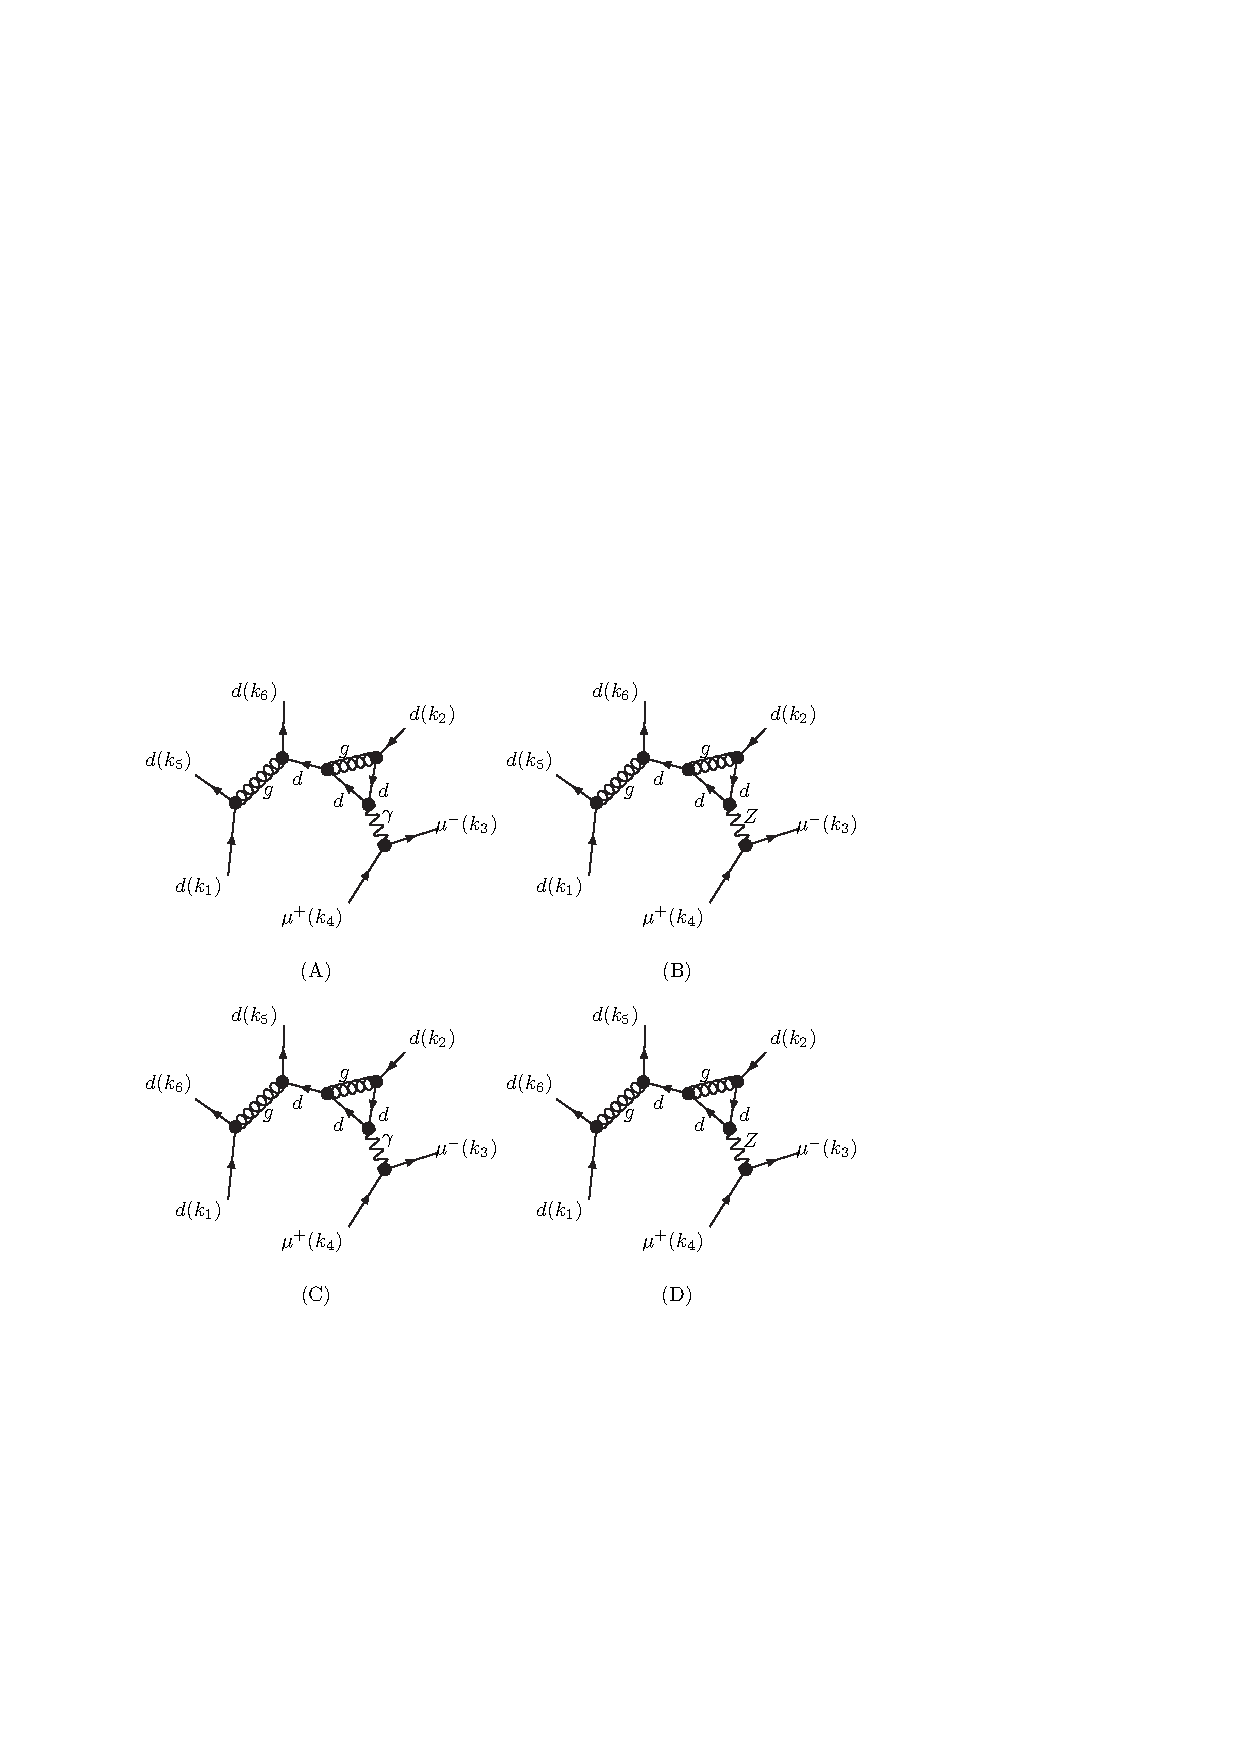
\includegraphics[width=1.0\textwidth]{diagsum1.pdf}
\caption{Example of diagrams sharing a common tree part, which are 
summed when the {\tt diagsum} option is set to {\tt diagsum=true}.}
\label{fig:diagsum_tree}
\end{figure} 

\begin{figure}[htb]
\centering
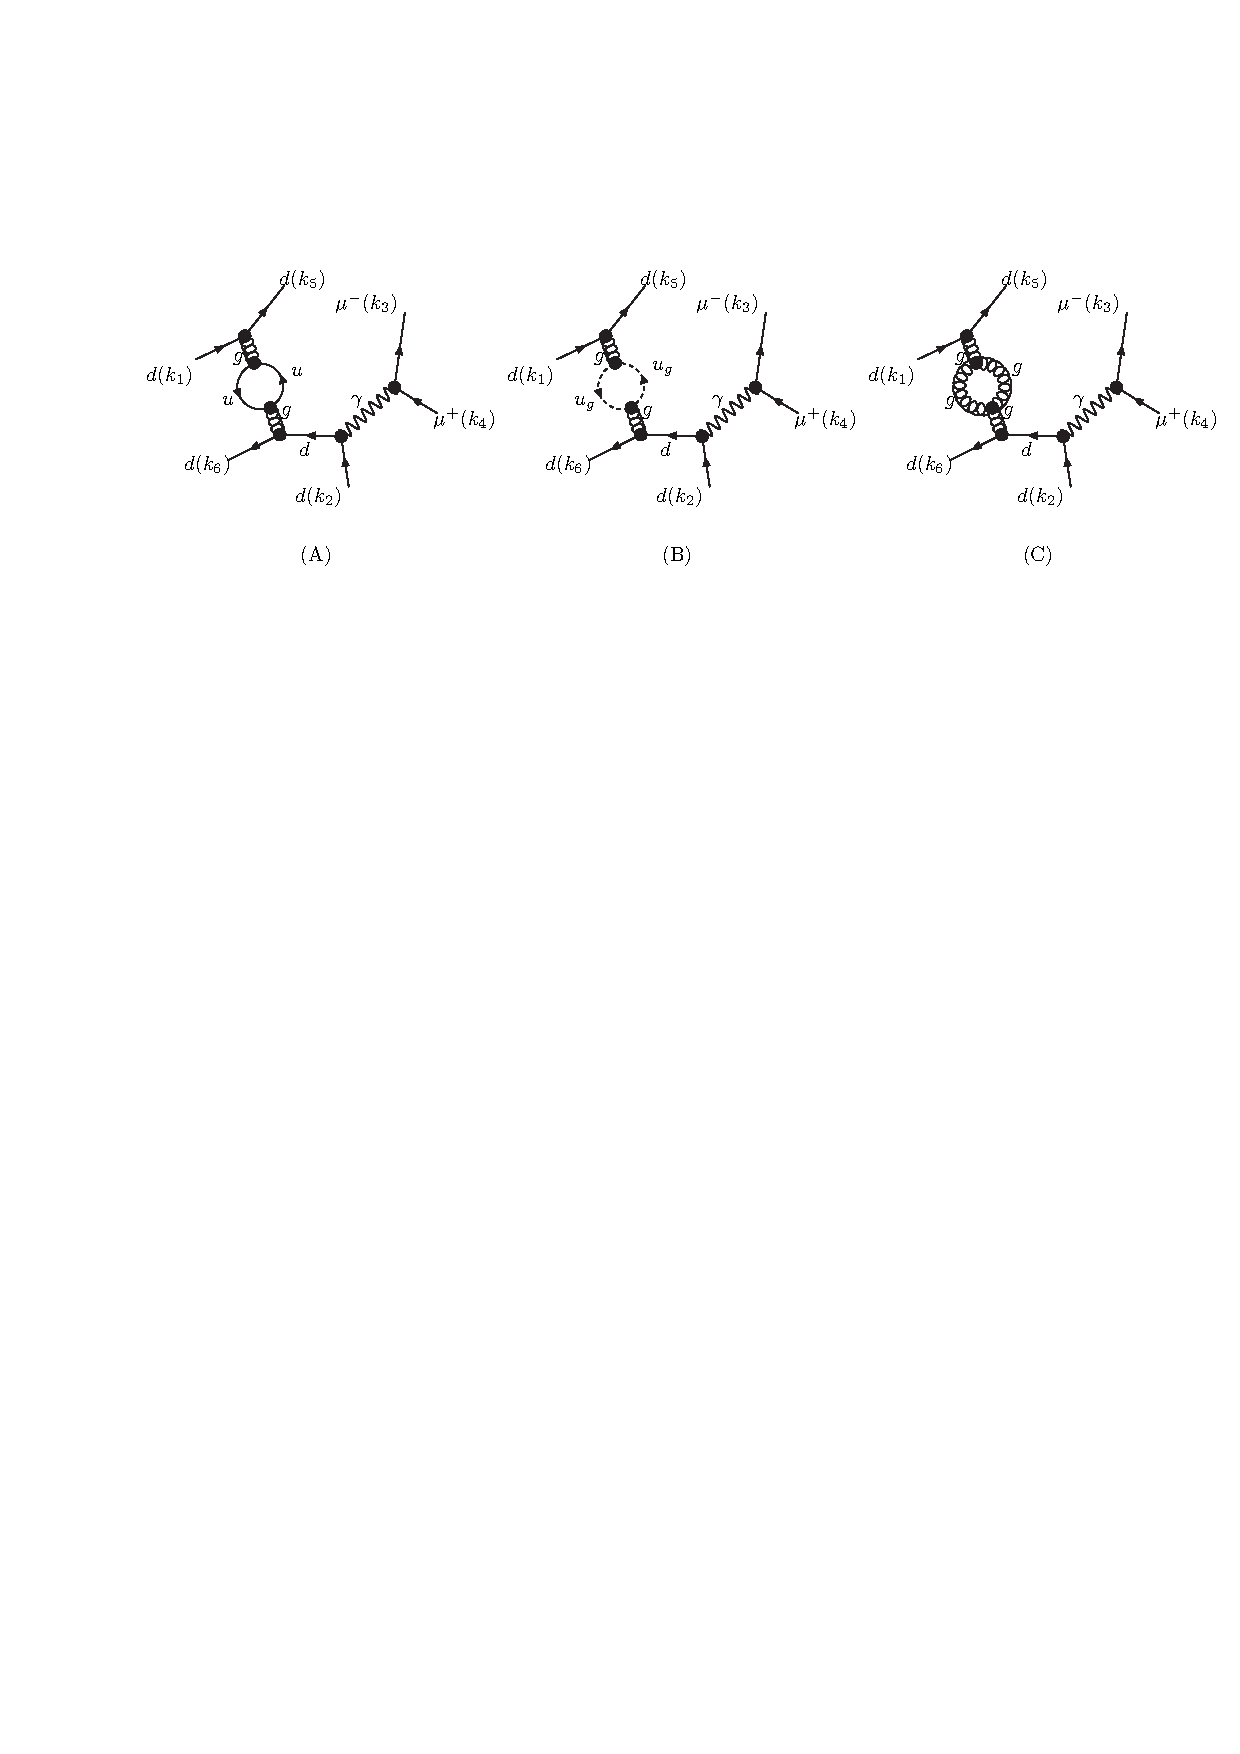
\includegraphics[width=1.1\textwidth]{diagsum2.pdf}
\caption{Example of diagrams sharing a common loop propagator, 
but with different particle content in the loop, which are summed when
the {\tt diagsum} option is set to {\tt diagsum=true}.}
\label{fig:diagsum_particle}
\end{figure} 


When the option {\tt diagsum} is active, diagrams which differ only by
a propagator external to the loop, as is the case e.g. for the
$Z/\gamma^\star$ propagator in QCD corrections to the production of
$Z+$jets, are summed together before being processed
by \form{}. Similarly, diagrams which differ only by an external tree
part, but which share exactly the same set of loop propagators, are
summed together prior the algebraic manipulation. An example is shown
Figure~\ref{fig:diagsum_tree}. Finally, diagrams which share the same
set of propagators, but have different particles circulating in the
loop, as shown in Figure~\ref{fig:diagsum_particle}, are also summed
into one ``meta-diagram''. The default setting for this option is {\tt
diagsum=true}.


\paragraph{Grouping of Tree Level Diagrams}

By default the expressions of all tree-level diagrams are grouped into one
file. This has the advantage that subexpressions which appear in several
tree-level diagrams can be reused across the amplitude. In some cases
it can happen that the sum of all terms of the tree-level diagrams is too big
to be compiled in one subroutine. In this case it is recommended to set
the option \texttt{group} to \texttt{false}. 
However, the latter can only be used in combination with the extension {\tt noformopt}.

\subsection{Numerical polarisation vectors}
\label{sec:numpolvec}
The use of numerical polarisation vectors for massless gauge bosons
(gluons, photons) is activated by default.  This means that the
various helicity configurations for the massless bosons will be
evaluated numerically, based on the same code, rather than producing
separate code for each helicity configuration.  In order to switch off
this default setting,
for example if the user would like to 
optimize the choice of reference vectors for each helicity configuration,
the option {\tt polvec=explicit} should be given in the process card 
{\tt process.in}.
In this case, \gosam{} will choose explicit reference vectors automatically.
If the user wants to specify his/her preferred reference vectors, 
this can be done using the option {\tt reference-vectors=\ldots}
in the process card.

\subsection{The extension {\tt derive}}

The {\tt derive} feature generates code to access the tensor coefficients
of each diagram or group of diagrams individually.
While it has been among the possible keywords for the 
{\tt extensions} option in \gosam-1.0 already, it now has been promoted to 
be used by default in the context of  tensorial reconstruction~\cite{Heinrich:2010ax}.
It improves both the speed and the
precision of tensorial reconstruction and makes connection to other reduction methods.

The idea behind it is to compute the numerator $\mathcal{N}(\hat{q})$ 
%--- we suppress the discussion of the second argument $\mu^2$ ---
from a Taylor series
\begin{equation}
\mathcal{N}(\hat{q})=\mathcal{N}(0)
+ \hat{q}^\mu
  \frac{\partial}{\partial\hat{q}_\mu}\mathcal{N}(\hat{q})\vert_{q=0}
+ \frac1{2!}\hat{q}^\mu\hat{q}^\nu
  \frac{\partial}{\partial\hat{q}_\mu}
  \frac{\partial}{\partial\hat{q}_\nu}
  \mathcal{N}(\hat{q})\vert_{q=0} + \ldots
\end{equation}
In this form one can read off a one-to-one correspondence between derivatives at
$\hat{q}=0$ and the coefficients of the tensor integrals.

%\paragraph{Implementation.}
At a technical level, 
the files \texttt{helicity*/d*h*l1d.f90} contain the routines
\texttt{derivative($\mu^2$, [$i_1$], [$i_2$],\dots)} and\\
\texttt{reconstruct\_d*(coeffs)}, where the latter is only generated in
conjunction with the extension \texttt{golem95}, and \texttt{coeffs} is
a type which comprises all coefficients of a diagram of a certain rank.
The number of optional indices $i_1$, $i_2$, \dots 
determine which derivative should be returned. The subroutine
\texttt{reconstruct\_d*} also takes into account the proper symmetrisation.

\subsection{Customization}\label{sec:Customization}
\paragraph{Runtime parameters.}
Many settings can be changed without recompiling the code, by
creating and modifying a file \texttt{matrix/param.dat}.
This file has a very simple format:
\begin{itemize}
\item Lines starting with a comment character (`!', `\#', `;')
      in the first column and blank lines are ignored.
\item All other lines have the format
\begin{example}
\textit{name} = \textit{float}\\
\# \textrm{or}\\
\textit{name} = \textit{float}, \textit{float}
\end{example}
      where the first line defines a real number and the second
      line defines a complex number, and \textit{name} is a defined
      parameter.
\item Whitespace is ignored but must not appear inside names or
      literals. Physical lines can not be continued nor can
      multiple entries appear on one line.
\end{itemize}
The list of recognized names can be found in the file
\texttt{common/model.f90}. 
With the built-in Standard Model file (\texttt{sm}) one
can re-set, for example, the value for the Higgs mass by 
{\tt mH = 125.5}.
All model constants that have not been specified as zero or one
can be set in this way. 
%Please note that upper and lower case letters have to be distinguished
%and that the names need to be spelled exactly as defined in \texttt{model.py}.
In addition there are some model independent parameters which can be found in the file 
\texttt{common/config.f90}.
%\smallskip

%\begin{tabular}{l@{\quad}p{0.7\textwidth}}
%   \texttt{samurai\_scalar} & selects a library of scalar integrals
%   (see \samurai documentation).\\
%   \texttt{samurai\_test} & sets a method to detect unstable points
%   (see \samurai documentation). \\
%   \texttt{samurai\_verbosity} & sets the verbosity level of
%   \samurai; it should be set to zero in a production environment
%   (see \samurai documentation).\\
%   \texttt{renormalisation} & An integer number indicating if no
%   renormalisation (0) or $\beta$-function renormalisation (1,
%   QCD only) should be applied. Other values are reserved for future
%   extensions. \\
%   \texttt{gauge\textit{i}o} & for the external vector particle with
%   index~$i$ (e.g. \texttt{gauge1o}, \texttt{gauge2o}\ldots),
%   if not defined as a constant. \\
%   \texttt{gauge\textit{i}z} & as \texttt{gauge\textit{i}o}.
%   The polarisation vector is transformed into
%   \begin{displaymath}
%   \varepsilon^\mu(k_i)\to\mathtt{gauge\mathit{i}o}\cdot\varepsilon^\mu(k_i)
%      + \mathtt{gauge\mathit{i}z}\cdot k_i^\mu
%   \end{displaymath}
%   This allows for a quick check of gauge invariance.
%\end{tabular}

\paragraph{Compile time parameters.}
Other configuration options can be found in the file \texttt{common/config.f90}.
%but require the recompilation of the source code
%(\texttt{make clean; make compile}).
\smallskip
Examples of options contained in \texttt{config.f90} are
\begin{maxipage}
\begin{tabular}{lp{0.6\textwidth}}
\texttt{ki} & the floating point kind used throughout the calculation, the default is double precision.\\
\texttt{debug\_lo\_diagrams} & controls if information about the
    tree level diagrams is written to the output file.\\
\texttt{debug\_nlo\_diagrams} & controls if information about the
    loop-diagrams is written to the output file.\\
\texttt{include\_eps\_terms} & controls if
    terms of order $\varepsilon$ multiplying
    poles are taken into account.\\
\texttt{include\_eps2\_terms} & controls if
    terms of order $\varepsilon^2$ multiplying
    double poles are taken into account.\\
\texttt{include\_color\_avg\_factor} & controls if the color averaging
    factor for inital state partons is multiplied to the final result.\\
\texttt{include\_helicity\_avg\_factor} & controls if the helicity averaging
    factor for inital state particles is multiplied to the final result.\\
\texttt{include\_symmetry\_factor} & controls if the symmetry
    factor for identical final state particles
    is multiplied to the final result. \\
\texttt{use\_sorted\_sum} & controls if the diagrams are summed using
    the algorithm Malcolm~\cite{Malcolm:1970}, which reduces the error
    accumulated in presence of large cancellations.\\
\texttt{tens\_rec\_by\_derivatives} & controls whether the tensorial reconstruction method is used.
\end{tabular}
\end{maxipage}

\section{Drawing the Feynman diagrams}
In order to print out the diagrams the makefile contains the target
\texttt{doc} which produces the file \texttt{process.pdf}.
We use \LaTeX{} plus the package \textsf{axodraw}~\cite{Vermaseren:1994je}
to create the graphical representation.

The layout of the diagrams is determined by the algorithm used in
\textsf{feynMF}~\cite{Ohl:1995kr}, modelling the propagators by springs.
The implemented algorithm works in two steps: first, the topology is
constructed by ordering the external legs such that the diagram can
be drawn as a planar graph. The coordinates $e_k$
of the external legs are
fixed along a contour around the drawing area.
%\footnote{Currently,
%this contour is chosen as an ellipse but in principle any convex shape could be used.}
In a second step the remaining degrees of freedom, the coordinates
of the vertices $v_i=(x_i, y_i)$, are fixed by minimizing the Lagrangian
\begin{multline}
L(v_1, \ldots, v_n; e_1, \ldots, e_N) =\\
 \frac14\sum_{i,j=1}^n t_{ij}\left(v_i-v_j\right)^2
+\frac12\sum_{i=1}^n\sum_{k=1}^N\lambda_{ik}\left(v_i-e_k\right)^2
\end{multline}
Here, $n$ is the number of vertices and $N$ is the number of external
legs.
Minimization of the Lagrangian leads to a system of linear equations, which
can easily be solved.
\begin{align*}
&\frac{\partial L}{\partial v_r}=0\\
\Leftrightarrow&
 \frac12\sum_{i,j=1}^n t_{ij}\left(v_i-v_j\right)
     \cdot\left(\delta_{ir}-\delta_{jr}\right)
+\sum_{i=1}^n\sum_{k=1}^N\lambda_{ik}\left(v_i-e_k\right)
     \cdot\delta_{ir}=0\\
\Leftrightarrow&
M_{rj}v_j\equiv
 \sum_{j=1}^n t_{rj}\left(v_r-v_j\right)
+\left(\sum_{k=1}^N\lambda_{rk}\right)v_r
=\sum_{k=1}^N\lambda_{rk}e_k
\end{align*}
In the last step we used the symmetry of $t_{ij}$.
The matrix $M$ can be written as
\begin{equation}
M_{rc}=\left\{\begin{array}{ll}
\left(\sum_{i\neq r}t_{ri}\right)+
\left(\sum_{k=1}^N\lambda_{rk}\right),&
r=c\\
-t_{rc},&\text{otherwise}
\end{array}\right.
\end{equation}

The symbol $t_{ij}$ is the sum of the spring constants of all
propagators connecting vertices $i$ and $j$; similarly, $\lambda_{ik}$
is the spring constant of the leg $k$ if it is connected to vertex $i$
and zero otherwise.

\section{Import of model files}
\label{sec:model}

The \gosam{}-\gosamversion{} package comes with the built-in model files 
{\tt sm}, {\tt smdiag}, {\tt smdiag\_mad}, {\tt smehc}, {\tt smdiagehc},
{\tt sm\_complex}, {\tt smdiag\_complex}, 
where the latter two are needed in the case of complex masses and couplings, 
see section \ref{sec:complexmasses}. 
The model files {\tt smdiag\_mad} contain some {\tt MadGraph5} specific settings, while
the model files {\tt smehc} and {\tt smdiagehc} contain the effective Higgs-gluon couplings.

Other models can be imported most easily in the {\tt UFO} (Universal FeynRules Output)~\cite{Degrande:2011ua,Darme:2023jdn} format.
The model import in the {\tt UFO} format can be used in the standalone as well as the OLP 
mode of \gosam, where both the BLHA1 and BLHA2 standards are supported for the syntax of the model import.

In order to perform calculations in an EFT like SMEFT or HEFT the user is required to provide the EFT model in the {\tt UFO} format. See section~\ref{sec:EFT} for more details.

Examples about how to import model files can be found in the subdirectory 
 \texttt{examples}.

\subsection{Import of a UFO model}\label{sec:UFO}
A model description in the UFO~\cite{Degrande:2011ua,Darme:2023jdn} format consists of a \texttt{Python} package
stored in a directory. In order to import the model into \gosam{} one needs
to set the \texttt{model} variable specifying the keyword \texttt{FeynRules}
in front of the directory name.
For example, if the \texttt{Python} model files for the MSSM are in 
 the directory \\
 \texttt{\$HOME/models/MSSM\_UFO}, the process card must contain the line
\begin{example}
model= FeynRules,\$HOME/models/MSSM\_UFO
\end{example}
All parameters of type ``external'' defined in the UFO model's \texttt{parameter.py} file will become available as runtime parameters (see section~\ref{sec:Customization}). To distinguish them from parameters defined within \gosam directly they are prepended with the prefix \texttt{mdl}. \gosam will try to figure out the correct naming of the strong (electroweak/QED) coupling by checking if the model contains any parameter, external or internal, denoted \texttt{G}, \texttt{GG} or \texttt{GS} (\texttt{E}, \texttt{EE}, \texttt{ee}).

In a UFO model each coupling is assigned a specific order, that is its power wrt. the QCD and/or QED coupling. In general more ``orders'' can be defined in the model, a feature which is useful to distinguish certain sets or classes of couplings. An example for an often used order is \texttt{NP}, which can be used to flag couplings of BSM or EFT origin. \gosam enables the user to make use of this UFO feature by means of the \python filter (see section~\ref{sec:filter}) \texttt{d.order('order')}, where \texttt{'order'} is a string denoting the name of the order parameter as defined in the UFO, e.g. \texttt{'NP'}. If the user wants to apply a filter based on a specific order, the property \texttt{order\_names} has to be declared in the process configuration file, e.g. \texttt{order\_names=NP}.

Note: \gosam is not able to handle arbitrarily large UFO models because of the limited buffer available in \qgraf. If the model is too large the user will be prompted an \qgraf error. In that case it might help to comment out vertices not contributing to the process from the UFO model files before starting \gosam.

\subsection{Import from LanHEP}
In order to use model files generated by LanHEP the following steps
have to be taken:
\begin{enumerate}
\item When generating the tables using LanHEP, one should include the
   following option to ensure that the generated tables have the correct
   headings\footnote{\gosamv{} relies on the column names rather than
   some specific order.}. The number of spaces in the column headers are
   irrelevant as long as the columns are wide enough to contain the
   respective values.
\begin{example}
   prtcformat\\
      fullname: '  fullname  ',\\
      name:     '  name   ',\\
      aname:    '  aname  ',\\
      spin2:    '  spin2  ',\\
      mass:     '  mass  ',\\
      width:    '  width  ',\\
      color:    '  color  ',\\
      aux:      '  aux  ',\\
      texname:  '      texname      ',\\
      atexname: '     atexname      ',\\
      pdg:      '  pdg   '.
\end{example}
\item If the model file is not already equipped with pdg codes
   the user might want to use the \verb!prtcprop! command in
   LanHEP to add the relevant codes.
\item In the setup file, one needs to specify the model as a pair
   of path and integer number. If the table files are under the directory
   \texttt{lanhep/ued/} in the tables \texttt{func7.mdl}, \texttt{lgrng7.mdl},
   \texttt{prtcls7.mdl} and \texttt{vars7.mdl}, the correct statement in
   the setup file would be
\begin{example}
   model=lanhep/ued, 7
\end{example}
\item The use of user defined functions (\texttt{external\_func} in LanHEP)
   requires an adaption of the file \texttt{codegen/haggies-l0.in}. If one
   wants to use the function \texttt{double foo(double,double)} the
   following line sould be added.
\begin{example}
@define mdlfoo : real, real -> real =\\ "foo(\%2\$s, \%3\$s)";
\end{example}
   The function also needs to be declared in \texttt{codegen/functions.out}
   in the subroutine \texttt{init\_functions}
\end{enumerate}


\subsection{Propagators for spin-2 particles}
\label{sec:spin2}

The propagator for massive spin-2 particles can be split into two parts
\begin{align}
	i \Delta_{\mu\nu,\rho\sigma}(k,m_{\vec n}) =  \underbrace{\frac{i}{k^2-m_{\vec n}^2 + i\epsilon}}_{D(k^2,m_{\vec n})} B_{\mu\nu,\rho\sigma}(k,m_{\vec n})\;,
\end{align}
where $B_{\mu\nu,\rho\sigma}$ carries the Lorentz structure
\begin{align}
	B_{\mu\nu,\rho\sigma}(k,m) =&
	             \left(\eta_{\mu \rho} - \frac{k_\mu k_\rho}{m^2}\right) 
		     \left(\eta_{\nu \sigma} - \frac{k_\nu k_\sigma}{m^2}\right)\notag \\
         &  + \left(\eta_{\mu \sigma} - \frac{k_\mu k_\sigma}{m^2} \right)
		     \left(\eta_{\nu \rho} - \frac{k_\nu k_\rho}{m^2}\right) \notag \\
         &  - \frac23  
	   \left(\eta_{\mu \nu} - \frac{k_\mu k_\nu}{m^2}\right)
	   \left(\eta_{\rho \sigma} - \frac{k_\rho k_\sigma}{m^2}\right)\;.
\end{align}
%and 
%\be
%D(s,m_{\vec n}) =  \frac{i}{s-m_{\vec n}^2 + i \epsilon}\;.
%\ee
If all particles attached to the propagator are on-shell, 
the mass dependent terms in $B_{\mu\nu,\rho\sigma}(k,m)$ drop out.
Further, if the on-shell condition is not always fulfilled, 
it turned out in phenomenological applications that the impact of the mass dependent terms is numerically 
negligible\,\cite{Gleisberg:2003ue,Greiner:2013gca}
and therefore we did not include them in our implementation
in order to avoid an enormous proliferation of terms.
In this case the summation over the graviton states  in $D(s,m_{\vec n})$, leading to
\be
D(s) = \sum_{\vec n} \frac{i}{s-m_{\vec n}^2 + i \epsilon}\;,
\ee
can be performed independently from the  $B_{\mu\nu,\rho\sigma}$ part carrying the Lorentz structure.
Further, in  models with large extra dimensions (LED),
 we can use the assumption that the widths of the KK modes are negligible, 
as the dominant effects come from the almost on-shell production of KK modes, 
and that the discrete spectrum of the KK  modes can be approximated by an
integral over a mass density, as the  KK modes are very contiguous.
%\,\cite{Han:1998sg,Giudice:1998ck}. 
The density as a function of the mass $m_{\vec n}$ is given by
\be
\rho(m_{\vec n})=\frac{R^{\delta}m_{\vec n}^{\delta - 2}}{(4\pi)^{\delta/2}\Gamma(\delta/2)}\;,
\ee
where $\delta$ is the number of extra dimensions, leading to \,\cite{Han:1998sg}
\begin{align}
	D(s) \to  \int_0^{M_S} d\,m_{\vec n}^2\,
	\frac{i\,\rho(m_{\vec n})}{s-m_{\vec n}^2+ i \epsilon}
	= \begin{cases} \frac{ s^{\delta/2-1}}{2M_{s}^{\delta + 2} G_N } \left( \pi + 2 i \, I(\frac{M_S}{\sqrt{s}}) \right) & \text{for\ } s>0 \\
		\frac{ (-s)^{\delta/2-1}}{2M_{s}^{\delta + 2} G_N} (-2i)\, I_E(\frac{M_S}{\sqrt{-s}}) & \text{for\ } s<0 
	\end{cases}
	\label{eq:propagator}
\end{align}
with 
\begin{align}
	I(x) = \begin{cases} - \sum_{k=1}^{\delta/2-1} \frac1{2k} x^{2k} - \frac12 \log(x^2-1)& \text{if\ } \delta \text{ even} \\
		- \sum_{k=1}^{(\delta-1)/2 } \frac{1}{2k-1} x^{2k-1} + \frac12 \log\left( \frac{x+1}{x-1} \right) & \text{if\ } \delta \text{ odd}
	\end{cases}
\end{align}
and
\begin{align}
	I_E(x) = \begin{cases} (-1)^{\delta/2 + 1} \left( \sum_{k=1}^{\delta/2-1} \frac{(-1)^k}{2k} x^{2k} + \frac12 \log(x^2+1)  \right) 
		& \text{if } \delta \text{ even} \\
		(-1)^{(\delta-1)/2} \left(   \sum_{k=1}^{(\delta-1)/2 } \frac{(-1)^k}{2k-1} x^{2k-1} + \frac12 \tan^{-1}(x) \right)   & \text{if } \delta \text{ odd} \,.
	\end{cases}
\end{align}
The UV cutoff $M_S$ is introduced as the effective theory approach loses its validity beyond the scale $M_S$.


\gosam{} supports spin-2 propagators with the \texttt{customspin2propagator} extension which
needs to be enabled in the process card by \\
{\tt extensions=customspin2propagator}.

The extension works only if the model is imported from an {\tt UFO} file. 
The latter can  be adjusted to the needs of the particular model the 
user would like to consider by editing the file {\tt custompropagator.f90}
in the subdirectory {\tt common}. 
In order to generate the latter file,
the spin-2 particle which should get a customized propagator needs to have a
separate attribute 'CustomSpin2Prop' in the {\tt UFO} file with a non-vanishing
value:\\
Excerpt of {\tt LED\_UFO/particle.py} with a customized propagator:
\begin{verbatim}
    Gr = Particle(pdg_code = 9000006,
                  name = 'Gr',
                  # ...
                  CustomSpin2Prop = 1
                 )
\end{verbatim}
Then \gosam{} generates a the file {\tt common/custompropagator.f90} where the user needs
to adapt the {\tt customSpin2Prop} subroutine.
Beside the squared momentum, the {\tt customSpin2Prop} subroutine also receives the
mass of the corresponding spin-2 particle as an argument, which
can be used to distinguish between multiple spin-2 particles if necessary.
The tensorial part of the spin-2 propagator, $B_{\mu\nu,\rho\sigma}(k,m_{\vec n})$, is treated separately 
and should not be modified.  If the user would like to modify it, we refer to the  documentation in 
section 6.3 of {\tt src/form/lorentz.pdf} in the \gosam{} tarball.



%\section{Handling big processes}
%Although the default settings should work for most cases, very big processes
%in terms of the number of diagrams and the size of the expressions can cause
%the compiler to become very slow or even to crash. In this section we discuss
%solutions which can help to reduce the load for the compiler and to speed-up
%the code generation. It should be mentioned that some of these measures can
%have a negative impact on the runtime efficiency of the generated code.



%%%%%%%%%%%%%%%%%%%%%%%%%%%%%%%%%%%%%%%%%%%%%%%%%%%%%%%%%%%%%%%%%%%%%%%%%%%

\chapter{Stability tests and rescue system}
\label{sec:rescue}

\gosam{} contains various options to assess in real time, for each phase space point, 
the level of precision of the corresponding one-loop matrix element. 
Whenever a phase space point is found in which the quality of the result falls below a
certain threshold, either the point is discarded or the evaluation of the amplitude is
repeated by means of a safer, albeit less efficient procedure. This procedure is
traditionally called ``rescue system''.

Apart from improvements in the stability of the reduction itself, which are provided by the new versions of \samurai{} and \golemVC, and in particular by the new reduction algorithm \ninja,  the new version of \gosam{} also has a more refined rescue system as compared to version 1.0. 

A first commonly used approach relies on the comparison between the numerical values of the
infrared pole coefficients computed by the one-loop program with 
their known analytic results dictated by the universal behaviour of the 
infrared singularities~\cite{Catani:2000ef}. We refer to this as the {\it pole test}. 

The main advantages of this method are its broad applicability and the fact that it requires a negligible additional computation time. However, since not all integrals which appear in the reconstruction of the amplitude give a contribution to the double and single poles, this method often provides an overestimate of the precision, which might result in keeping  phase space points whose finite part is less precise than what is predicted by the pole test.

To target directly the precision of the finite part, various possibilities exist.
Using the symmetry properties of scattering amplitudes under scaling of all physical scales,
 or alternatively the invariance under rotation of the momenta, 
 we can build pairs of points that should provide identical results, 
 both for the finite parts and for the poles, and use the difference between them 
 as an estimator of the precision. 

The {\it scaling test}~\cite{Badger:2010nx}, is based on the properties of scaling of scattering amplitudes when all physical scales (momenta, renormalization scale, masses) are rescaled by a common multiplicative factor $x$. As shown in~\cite{Badger:2010nx}, this method provides a very good correlation between the estimated precision and the actual precision of the finite parts.

The {\it rotation test}~\cite{vanDeurzen:2013saa} exploits the invariance of the scattering amplitudes under an azimuthal rotation about the beam axis, namely the direction of the initial colliding particles. Whenever the initial particles are not directed along the beam axis, one can perform a rotation of all particles by an arbitrary angle in the space of momenta. A validation of this technique, and the corresponding correlation plots, has been presented in~\cite{vanDeurzen:2013saa}.

While  the {\it scaling} and the {\it rotation test} provide a more reliable estimate of the precision of the finite parts that enter in the phase space integration, their downside is that they require two evaluations of the same matrix element, therefore leading to a doubling in the computational time.

%Additional methods have been proposed, within the context of integrand-reduction approaches, which target the relations between the coefficients before integration, namely the reconstructed algebraic expressions for the numerator function before integration, known as  $\N=\N$ tests~\cite{Ossola:2007ax, Mastrolia:2010nb}.
%This kind of tests can be applied to the full amplitude (global   $\N=\N$ test) or individually within each residue of individual cuts (local $\N=\N$ test). The drawback of this technique comes from the fact that the test is applied at the level of individual diagrams, rather than on the final result summed over all diagrams, making the construction of a rescue system quite cumbersome. 

For the precision analysis contained in \gosamv, and to set the trigger for the rescue system, we decided to employ  a hybrid method, that takes advantage of the computational speed of the {\it pole test}, combined with the higher reliability of the {\it rotation test}.  This hybrid method requires setting three different thresholds.
After computing the matrix elements, \gosamv{} checks the precision  $ \delta_{pole}$ of the single pole with the {\it pole test}. Comparing the single pole 
$\S_{IR}$ that can be obtained from the general structure of infrared singularities and the one provided by  \gosamv, which we label $\S$, we define  
\be \label{eq:exd}
\delta_{pole} = \left | \frac{ \S_{IR} - \S{} }{ \S_{IR}} \right |\, .
\ee
The corresponding estimate of the number of correct digits in the result is provided by  $P_{pole}= - \log_{10} (\delta_{pole})$. This step does not require any increase in computational time. The value of $ P_{pole}$ is then compared with two thresholds $ P_{high}$ and $ P_{low}$. 

If $P_{pole} >  P_{high}$ the point is automatically accepted. Given the high quality of the computed pole, the finite part is very unlikely to be so poor that the point should be discarded.

If $P_{pole} <  P_{low}$ the point is automatically discarded, or sent to the rescue system. If already the pole has a low precision, we can expect the finite part to be of the same level or worse.
 
In the intermediate region where $ P_{high} > P_{pole} >  P_{low}$, it is more difficult to determine the quality of the result solely based on the pole coefficients. Only in this case the point is recalculated using the {\it rotation test}, which requires additional computational time. 

If we call the finite part of the amplitudes evaluated before and after the rotation $\A$ and  $\A_{rot}$ respectively,  we can define the error $ \delta_{rot}$ estimated with the rotation  as  
\be  \label{eq:errd} \delta_{rot} =  2 \left  |\frac{ A_{rot} - A }{ A_{rot} + A} \right  |\, . \ee
and the corresponding estimate on the number of correct digits as $P_{rot} = - \log_{10} (\delta_{rot})$.
$P_{rot}$ provides a reliable estimate of the precision of the finite part~\cite{vanDeurzen:2013saa}, and can be compared with a threshold $P_{set}$ to decide whether the point should be accepted or discarded. 

The values of the three thresholds $ P_{high} $,  $P_{low}$ and $P_{set}$ can be chosen by the user, to adjust the selection mechanism to the fluctuations in precision which occur between different processes. In the input card, $ P_{high} $,  $P_{low}$ and $P_{set}$ correspond to 
\texttt{PSP\_chk\_th1}, \texttt{PSP\_chk\_th2} and \texttt{PSP\_chk\_th3}, 
respectively, see section \ref{chp:setup-of-a-process}.
It is worth to notice that the {\it rotation test} can be bypassed simply by setting the initial thresholds $P_{high}= P_{low}$. In this case the selection is performed solely on the basis of the {\it pole test}.


%%%%%%%%%%%%%%%%%%%%%%%%%%%%%%%%%%%%%%%%%%%%%%%%%%%%%%%%%%%%%%%%%%%%%%%%%%%
\chapter{Electroweak corrections}


\section{Electroweak scheme choice}
\label{sec:ewchoose}
When computing amplitudes within the Standard Model, there are different
possibilities how to choose which electroweak parameters are
considered as input parameters, and which are instead derived
ones. Within \gosam{} different schemes can be chosen in several
different ways, depending on whether the scheme might be changed after
the generation of the code or not, by setting appropriately the flag
{\tt model.options}.

By default, when the flag is not set in the input card, \gosam{}
generates a code which uses $\mrm{m_W}$, $\mrm{m_Z}$ and
$\mrm{\alpha}$ as input parameters, allowing however to change this in
the generated code, by setting the variable {\tt ewchoice} in the
configuration file {\tt config.f90} to the desired value. The user can
choose among 8 different possibilities, which are listed in
Table~\ref{tab:ewchoose}.  When the electric charge $\mrm{e}$ is set
algebraically to one, the schemes $6-8$ cannot be used.

\begin{table*}
\begin{center}
\small
\begin{tabular}{|c|l|l|}
\hline
ewchoice & input parameters                        & derived parameters                  \\
\hline
1        & $\mrm{G_F}$, $\mrm{m_W}$, $\mrm{m_Z}$    & $\mrm{e}$, $\mrm{sw}$              \\
2        & $\mrm{\alpha}$, $\mrm{m_W}$, $\mrm{m_Z}$ & $\mrm{e}$, $\mrm{sw}$              \\
3        & $\mrm{\alpha}$, $\mrm{sw}$, $\mrm{m_Z}$  & $\mrm{e}$, $\mrm{m_W}$             \\
4        & $\mrm{\alpha}$, $\mrm{sw}$, $\mrm{G_F}$  & $\mrm{e}$, $\mrm{m_W}$             \\
5        & $\mrm{\alpha}$, $\mrm{G_F}$, $\mrm{m_Z}$ & $\mrm{e}$, $\mrm{m_W}$, $\mrm{sw}$ \\
6        & $\mrm{e}$, $\mrm{m_W}$, $\mrm{m_Z}$      & $\mrm{sw}$                         \\
7        & $\mrm{e}$, $\mrm{sw}$, $\mrm{m_Z}$       & $\mrm{m_W}$                        \\
8        & $\mrm{e}$, $\mrm{sw}$, $\mrm{G_F}$       & $\mrm{m_W}$, $\mrm{m_Z}$           \\
\hline
\end{tabular}
\end{center}
\caption{Possible choices to select the electroweak scheme.
To simplify the notation we write the sine of the Weinberg angle as
$\mrm{sw}$. The lists of derived parameters contain only the
parameters which are computed and used in the expressions for the
amplitudes.}\label{tab:ewchoose}
\end{table*}


The flag {\tt model.options} in the input card allows also to directly
set the values of the different parameters appearing in the model. If
the values of exactly three electroweak parameters are
specified, \gosam{} automatically takes them as input parameters. In
that case, in order to be able to switch among different schemes after
code generation, the variable {\tt ewchoose} also must be added to the
{\tt model.options} flag.



\section{Support of complex masses}
\label{sec:complexmasses}
The integral libraries contained in the \gosam{} package as well as the \gosam{} 
code itself fully support complex masses. This refers to the introduction of 
finite widths for fermions as well as
for $W$- and $Z$-bosons. A fully consistent treatment of complex
$W$- and $Z$-boson masses requires the use of the complex mass scheme~\cite{Denner:2005fg}.
The boson masses are promoted to complex masses by
\begin{equation}
 m_{V}^2 \to \mu_{V}^2 = m_{V}^2 -i m_{V} \Gamma_{V},\quad V=W,Z\;.
\end{equation}
In order to maintain gauge invariance this affects the definition of the Weinberg angle:
\begin{equation}
 \cos^2\theta_w = \frac{\mu_W^2}{\mu_Z^2}\;.
\end{equation}
 To make use of the complex mass scheme, we introduce two new model files, \texttt{sm\_complex}
 and \texttt{smdiag\_complex}, which contain the Standard Model with complex mass scheme, the first
 with a full CKM matrix, the latter with a diagonal  CKM matrix.
 An example dealing with a complex top quark mass is given in 
 the {\tt examples/singletop} subdirectory of the \gosam{} distribution.

%\subsection{Splitting the Process}
%If a process becomes too big in order to be linked\footnote{
%Currently, most systems support programs to a size up to 4\,GB.
%Although 64\,bit systems can handle a much bigger address space,
%the current limitation comes from some legacy code in the GNU linker.}
%there are some possibilities to split the process into independent
%programs:
%\begin{itemize}
%\item the generation of a subset of the helicity configurations, 
%e.g. one helicity configuration      per process directory.
%\item the generation of a subset of diagrams. If the diagrams are not
%      split according to gauge invariant subsets the user should ensure
%      that all subsets are called with the same set of phase space points.
%      An easy way of splitting the diagrams into subsets is by using
%      the option \texttt{select.nlo=\textit{$\langle$first$\rangle$}:\textit{%
%       $\langle$last$\rangle$}}, where \texttt{first} and \texttt{last} refer to the 
%       diagram numbers in {\em process.ps}.
%\end{itemize}

%\section{Advanced Usage}
%The call to the executable \texttt{gosam.py} can be simulated
%inside more complex \python programs.
%It is an easy exercise to
%run the file generation in user defined \python scripts as long as
%one includes the module files in the environment variable
%\texttt{PYTHON\_PATH}. The following script emulates the
%program \texttt{gosam.py}:
%\begin{lstlisting}[language=python]
%>>> from golem.util.config import Properties
%>>> from golem.util.main_misc import *
%>>> props = Properties()
%>>> props.setProperty("in", ["e+", "e-"])
%>>> props.setProperty("out", ["t", "t~"])
%>>> # ... populate props with further values ...
%>>> workflow(props)
%>>> generate_process_files(props)
%\end{lstlisting}

\chapter{Advanced diagram selection}
\gosam generates all diagrams consistent with the coupling orders and external states by default. If only a subset of these diagrams are to be considered, several ways of restricting the diagrams are provided:
\begin{itemize}
   \item Selecting specific diagrams by their IDs
   \item Restricting diagrams with the \texttt{filter.particles} flags
   \item Filtering the diagrams using \qgraf's built-in options
   \item Filtering the diagrams using custom \python functions
\end{itemize}
The four options are listed in increasing flexibility, but also increasing complexity. All mentioned process card options are described in more detail in appendix \ref{chp:process_card_options}.

\section{Selecting diagrams by their number}
The easiest way to remove some diagrams from a process is with the \texttt{select[.lo|.nlo|.ct]} options. These options take a set of diagram IDs to determine which diagrams are kept in the respective component. A convenient way to inspect the diagram IDs is \texttt{doc/process.pdf}, which contains all diagrams with their respective identifiers. After modifying the \texttt{select} options and rerunning \texttt{gosam.py}, only the specified diagrams are kept. 

\section{Filtering diagrams with the \texttt{filter.particles} options}
To discard multiple diagrams based on the internal propagators, the \texttt{filter[|.lo|.nlo|.ct].particles} options can be used. These options discard diagrams which do not have the specified number of internal propagators of the given field. These options are applied at the diagram generation level and are therefore more efficient compared to an equivalent \python filter.

\section{Restricting the generation with \qgraf}
\qgraf itself also allows filtering the diagrams it generates. These options are described in the \qgraf manual and can be applied with the \texttt{qgraf.verbatim[.lo|.nlo|.ct]} options. The content of these options is written verbatim to \qgraf's input file for the respective component. 

Since these filters are applied already in the first of the diagram generation, they are more efficient compared to an equivalent \python filter. Since this difference is largely insignificant on modern CPUs, it is nevertheless recommended using the \python filters.

\section{Filtering diagrams in \python{}}
\label{sec:filter}
The final implemented diagram selection option are the \python filters. They allow arbitrary diagram selection criteria by using user-supplied custom \python functions. They are supplied with the \texttt{filer[.lo|.nlo|.ct]} options, which expects a \python function \begin{lstlisting}[style=py]
   filter(d: golem.topolopy.objects.Diagram) -> bool: ...
\end{lstlisting}
Diagrams for which this function returns \texttt{True} are kept, diagrams for which \texttt{False} is returned are discarded.

If the filter function is sufficiently simple, it can directly be supplied to the \texttt{filter} option via a \python lambda-function. If the filter function becomes too complicated, it can be moved to an external file. The name of this file can then be supplied with the \texttt{filter.module} option, after which the functions defined in this external file can be used in the \texttt{filter} options.

\subsection{Methods for diagram filtering}
The custom filter functions receive a single \texttt{Diagram} object as input. Many convenience methods are implemented on this object to simplify the construction of filters. In the following, a field can be specified as 
\begin{lstlisting}[style=py]
   Field = str | Sequence[str]
\end{lstlisting}
where each string is the name of the respective field. If multiple field names are supplied, any field from the sequence will be tested for a match.

\emph{Note that Python will not necessarily return an exception if this format is not respected, but the filters might not work as expected.} 

\subsubsection{\texttt{golem.topolopy.objects.Diagram}}
\begin{adjustwidth}{-100pt}{0pt}
\begin{basedescript}{\desclabelstyle{\pushlabel}}
   \item[\hspace{-1em}]\colorbox{gray!30}{\lstinline[style=py]|rank() -> int|} \vspace{0.1cm}\\
   Return the tensor rank of a diagram.

   \item[\hspace{-1em}]\colorbox{gray!30}{\lstinline[style=py]|sign() -> int|} \vspace{0.1cm}\\
   Return the sign of a diagram.

   \item[\hspace{-1em}]\colorbox{gray!30}{\lstinline[style=py]|isNf() -> bool|} \vspace{0.1cm}\\
   Return \texttt{True} if the diagram contains a massless closed fermion loop of size two.

   \item[\hspace{-1em}]\colorbox{gray!30}{\lstinline[style=py]|isMassiveQuarkSE() -> bool|} \vspace{0.1cm}\\
   Return \texttt{True} if the diagram contains a QCD self-energy insertion on a massive quark line.

   \item[\hspace{-1em}]\colorbox{gray!30}{\lstinline[style=py]|isScaleless() -> bool|} \vspace{0.1cm}\\
   Return \texttt{True} if the diagram contains a scaleless loop integral.

   \item[\hspace{-1em}]\colorbox{gray!30}{\lstinline[style=py]|vertices(*fields: Field) -> int|} \vspace{0.1cm}\\
   Returns the number of vertices in the diagram for which the fields match the given field patterns. \vspace{0.1cm} \\
   Example:
   \begin{lstlisting}[style=py]
    # Remove all diagrams with u Yukawa vertices
    lambda d: d.vertices(["U", "Ubar"], ["U", "Ubar"], "H") == 0
   \end{lstlisting}

   \item[\hspace{-1em}]\colorbox{gray!30}{\lstinline[style=py]|loopvertices(*fields: Field) -> int|} \vspace{0.1cm}\\
   Same as \texttt{vertices}, but only vertices that are part of the loop are considered.

   \item[\hspace{-1em}]\colorbox{gray!30}{\lstinline[style=py]|iprop(f: Field, **opts) -> int|} \vspace{0.1cm}\\
   Returns the number of propagators in the diagram for which the fields match the given field patterns. Additional properties of the propagators can be specified with \texttt{**opts}, only propagators matching the additional restrictions are counted. The available keywords are \\
   \def\arraystretch{1.5}
   \begin{tabular}{l l}
    \colorbox{gray!30}{\lstinline[style=py]|momentum: str|} & Momentum of the propagator. \\
    \colorbox{gray!30}{\lstinline[style=py]{twospin: int | Sequence[int]}} & Twice the spin of the propagator. \\
    \colorbox{gray!30}{\lstinline[style=py]{color: int | Sequence[int]}} & Color representation of the propagator. \\
    \colorbox{gray!30}{\lstinline[style=py]|massive: bool|} & Massive Propagators.
   \end{tabular}
   \def\arraystretch{1.0}
   \vspace{0.2cm} \\
   Example:
   \begin{lstlisting}[style=py]
    # Remove all diagrams first generation propagators with momentum k1+k2
    lambda d: d.iprop(["U", "Ubar", "D", "Dbar"], momentum = "k1+k2") == 0
   \end{lstlisting}
   \colorbox{red!15}{\parbox{\linewidth}{\textbf{Warning}: \vspace{0.1cm}\\ \gosam relates some subprocesses to their crossing by default. Using the \texttt{momentum} keyword can break the crossing symmetry and therefore falsify the result. In this case, either run \gosam with the \texttt{no-crossings} option or use the \lstinline[style=py]|iprop_momentum| function.}}

   \item[\hspace{-1em}]\colorbox{gray!30}{\lstinline[style=py]|iprop_momentum(f: Field, momentum: str) -> bool|} \vspace{0.1cm}\\
   Returns \texttt{True} if the diagram contains a propagator of the given field with the given momentum. When \texttt{True} is returned, the diagram is flagged as potentially crossing symmetry violating and all subprocesses related to the one containing the current diagram are tested for crossing symmetry explicitly.

   \item[\hspace{-1em}]\colorbox{gray!30}{\lstinline[style=py]|chord(f: Field, **opts) -> int|} \vspace{0.1cm}\\
   Same as \texttt{iprop}, but only counts loop propagators.

   \item[\hspace{-1em}]\colorbox{gray!30}{\lstinline[style=py]|bridge(f: Field, **opts) -> int|} \vspace{0.1cm}\\
   Same as \texttt{iprop}, but only counts non-loop propagators.

   \item[\hspace{-1em}]\colorbox{gray!30}{\lstinline[style=py]|order(coupling: str) -> int|} \vspace{0.1cm}\\
   Returns the order of the diagram in the given coupling.

   \item[\hspace{-1em}]\colorbox{gray!30}{\lstinline[style=py]|QuarkBubbleMasses() -> list[str]|} \vspace{0.1cm}\\
   Returns a list of the propagator masses in a quark loop of size two. If the diagram does not contain such a loop, an empty list is returned.  

   \item[\hspace{-1em}]\colorbox{gray!30}{\lstinline[style=py]{ext_legs_from_vertex(f: Field, max_legs=1, is_ingoing=None) -> bool}} \vspace{0.1cm}\\
   Returns \texttt{True} if more than \texttt{max\_legs} legs matching \texttt{f} are attached to the same vertex. For \lstinline[style=py]| is_ingoing == True| only incoming legs are counted, for \lstinline[style=py]| is_ingoing == False| only outgoing legs are counted. All legs are counted when \texttt{is\_ingoing} is \texttt{None}. The diagram is automatically flagged for potential crossing symmetry violation if \texttt{True} is returned and \texttt{is\_ingoing} is not \texttt{None}.

   \item[\hspace{-1em}]\colorbox{gray!30}{\lstinline[style=py]{vertex_with_external_legs(*fields: Field, **opts) -> bool}} \vspace{0.1cm}\\
   Returns \texttt{True} if more than \texttt{max\_legs} legs are attached to a vertex matching \texttt{*fields}. The keywork options are the same as for \texttt{ext\_legs\_from\_vertex}. For \lstinline[style=py]| is_ingoing == True| only incoming legs are counted, for \lstinline[style=py]| is_ingoing == False| only outgoing legs are counted. All legs are counted when \texttt{is\_ingoing} is \texttt{None}. The diagram is automatically flagged for potential crossing symmetry violation if \texttt{True} is returned and \texttt{is\_ingoing} is not \texttt{None}.

   \item[\hspace{-1em}]\colorbox{gray!30}{\lstinline[style=py]|loopsize() -> int|} \vspace{0.1cm}\\
   Returns the size of the loop.
\end{basedescript}

\end{adjustwidth}

%%%%%%%%%%%%%%%%%%%%%%%%%%%%%%%%%%%%%%%%%%%%%%%%%%%%%%%%%%%%%%%%%%
%% BLHA.tex is a separate file, was used for the version 1.0 manual
%\documentclass[a4paper]{refart}
%\usepackage{listings}
%\usepackage{color}
%\usepackage{amsmath}
%\title{GoSam BLHA Interface How-To}
%\author{T. Reiter, G.~Luisoni}
%\definecolor{lstbg}{rgb}{0.9,0.9,0.9}
%\lstset{basicstyle=\tt,backgroundcolor=\color{lstbg}}
%\begin{document}
%\maketitle
%\tableofcontents

\chapter{The Binoth Les Houches Accord Interface}
\label{sec:blha}


The interface of \gosam{} with a Monte Carlo event generator program 
is based on the Binoth-Les Houches Accord (BLHA)
standard interface.
\gosam{}-\gosamversion supports both BLHA1~\cite{Binoth:2010xt}
and BLHA2~\cite{Alioli:2013nda}.
Certainly, a dedicated interface without using the BLHA is also possible.

%We assume that \gosam{} has been downloaded and installed using the script
%\texttt{gosam-installer.py} which comes with the distribution. 
%You should ensure
%that the file \texttt{gosam.py} is in your \texttt{\$PATH} variable.


\section{Preparation of the order file}
This step should be done by the Monte Carlo (MC) program. 
We give a generic example of an order file for the process \\
$pp\to (Z\to e^+e^-)+$\,jet in both BLHA1 and BLHA2 standards 
in Figs.~\ref{fig:BLHA1} and \ref{fig:BLHA2}.
%in the files \texttt{order1.lh} \texttt{order2.lh}  
\begin{figure}[htb!]
\begin{subfigure}[]{0.49\textwidth}
%\framebox(158,210){%
\fbox{
    \parbox[t][][c]{145\unitlength}{\tt\scriptsize
\# OLP\_order.lh   \\
\# created by MC Sherpowig-1.0\\
\# Process: p p $->$ e+ e- jet\\
Model                    SMdiag\\
CorrectionType           QCD\\
IRregularisation         DRED\\
AlphasPower              2\\
AlphaPower               1\\
MatrixElementSquareType  CHsummed\\
OperationMode            CouplingsStrippedOff\\
SubdivideSubprocess      no\\
\# Subprocesses \\
1 -1 $->$ 11 -11 21\\ 
1 21 $->$ 11 -11 1\\
2 -2 $->$ 11 -11 21\\
...\\
21 -2 $->$ 11 -11 -2\\
\\
\# Process specific GoSam settings\\
\#@ symmetries family,generation}
}
\end{subfigure}
\begin{subfigure}[]{0.49\textwidth}
%\framebox(178,210){%
\fbox{
    \parbox[t]{165\unitlength}{\tt\scriptsize
\# vim: syntax=olp\\
\#@OLP GOSAM 2.0\\
\#@IgnoreUnknown False\\
\#@IgnoreCase False\\
\#@SyntaxExtensions \\
CorrectionType QCD $|$ OK\\
IRregularisation DRED $|$ OK\\
AlphasPower 2 $|$ OK\\
AlphaPower  1   $|$ OK\\           1\\
MatrixElementSquareType CHsummed $|$ OK\\
OperationMode CouplingsStrippedOff $|$ OK\\
SubdivideSubprocess  no $|$ OK\\
1 -1 $->$ 11 -11 21 $|$ 1 1\\
1 21 $->$ 11 -11 1  $|$ 1 2\\
2 -2 $->$ 11 -11 21 $|$ 1 3\\
...\\
21 -2 $->$ 11 -11 -2 $|$ 1 13\\}
}
\end{subfigure}
\caption{Examples of order and contract files for Z+jet, with BLHA1 standards.}
\label{fig:BLHA1}
\end{figure}  



\begin{figure}[h]
\begin{subfigure}[]{0.49\textwidth}
%\framebox(150,310){%
\fbox{
    \parbox[t][][b]{148\unitlength}{\tt\scriptsize
\#  OLP\_order.lh \\
\# created by MC Sherpowig-2.0\\
InterfaceVersion         BLHA2\\
CorrectionType           QCD\\
IRregularisation         DRED\\
WidthScheme              ComplexMass\\
EWScheme                 alphaGF\\
AccuracyTarget           0.0001\\
DebugUnstable            True\\

AlphasPower              1\\
AmplitudeType ccTree\\
1 -1 $->$ 11 -11 21 \\
...\\
21 -2 $->$ 11 -11 -2 \\
AmplitudeType scTree\\
1 -1 $->$ 11 -11 21 \\
...\\
21 -2 $->$ 11 -11 -2 \\
AmplitudeType Loop\\
1 -1 $->$ 11 -11 21 \\
...\\
21 -2 $->$ 11 -11 -2 \\
\\
AlphasPower              2\\
AmplitudeType Tree\\
1 1 $->$ 11 -11 1 1 \\ 
...\\
21 21 $->$ 11 -11 2 -2\\}}
\end{subfigure}
%\parbox{5\unitlength}{}
\begin{subfigure}[]{0.49\textwidth}
%\framebox(163,310){%
\fbox{
    \parbox[t][][b]{160\unitlength}{\tt\scriptsize
\# vim: syntax=olp\\
\#@OLP GOSAM 2.0\\
\#@IgnoreUnknown False\\
\#@IgnoreCase False\\
\#@SyntaxExtensions \\
InterfaceVersion BLHA2 $|$ OK\\
CorrectionType QCD $|$ OK\\
IRregularisation DRED $|$ OK\\
WidthScheme              ComplexMass $|$ OK\\
EWScheme                 alphaGF $|$ OK\\
AccuracyTarget           0.0001 $|$ OK\\
DebugUnstable            True $|$ OK\\

AlphasPower 1 $|$ OK\\
AmplitudeType ccTree $|$ OK\\
1 -1 $->$ 11 -11 21 $|$ 1 131\\
...\\
21 2 $->$ 11 -11 2 $|$ 1 70\\
AmplitudeType scTree | OK\\
1 -1 $->$ 11 -11 21 $|$ 1 145\\
...\\
21 2 $->$ 11 -11 2 $|$ 1 71\\
AmplitudeType Loop $|$ OK\\
1 -1 $->$ 11 -11 21 $|$ 1 137\\
...\\
21 2 $->$ 11 -11 2 $|$ 1 63\\
\\
AlphasPower 2 $|$ OK\\
AmplitudeType Tree $|$ OK\\
1 1 $->$ 11 -11 1 1 $|$ 1 42\\
...\\
21 21 $->$ 11 -11 -2 2 $|$ 1 106\\}
}
\end{subfigure}
\caption{Order and contract files for Z+jet with BLHA2 standards.}
\label{fig:BLHA2}
\end{figure}  

\paragraph{Remarks}
\begin{itemize}
\item The order file can have any name and any extension.
      We use  the extension \texttt{.lh}
      for order files and \texttt{.olc} for contract files.
\item The options \texttt{WidthScheme, EWScheme} in the BLHA2  example are optional.
\item The option \texttt{SubdivdeSubprocess}  has the following effect
      on the code generation with \gosam{}: if set to 
      \texttt{no}, \gosam{} generates one label per subprocess, if set to
      \texttt{yes} it generates one label per helicity subamplitude
      and therefore \emph{many} labels per subprocess.
      
\item \gosam{} specific settings can be put into commentary lines starting
      with the letter combination `\texttt{\#@}'. This is not part of the
      BLHA standard. The line `\texttt{\#@ symmetries} \dots' restricts the
      helicity subamplitudes being generated to the ones relevant for this
      particular process, using the information that flavour changings only occur within 
      the same quark families resp. lepton generations.

      Additionally, the \texttt{Extra} keyword of BLHA2 for OLP-specific settings is also supported.
%      The command \texttt{\#@ filter.nlo NOT(SCALELESS)}
%      excludes scaleless diagrams from the amplitude generation,as they will be zero anyway.
\end{itemize}

\clearpage

\section{Running GoSam}
To run \gosam{} within the MC/OLP setup one can use the following command:\\
%\begin{lstlisting}[language=bash]
{\tt gosam.py --olp --mc=MCname }\\
\contl{\tt    --config=<your-path-to>/gosam.conf order.lh}
%\end{lstlisting}

\paragraph{Remarks}
\begin{itemize}
\item The extension \texttt{--olp} is mandatory whenever 
   a BLHA order file is processed.
\item The extension \texttt{--mc=MCname} is optional. By specifying the
   name of the Monte Carlo which is the intended partner program,
   \gosam{} can choose some settings simplifying the communication and linking.
   One can either specify \texttt{--mc=MCname} or \texttt{--mc=name/version}.
   Alternatively (and also optional),
   one can put this information into the order file:\\
%\begin{lstlisting}
{\tt \#@olp.mc.name mypreferredmc}\\
{\tt \#@olp.mc.version 1.0.0}\\
%\end{lstlisting}
   The short option for \texttt{--mc} is \texttt{-M}.
%   The supported MC names so far are {\tt powhegbox, sherpa}.
%   The interface with Herwig++/Matchbox does not need any extra settings when using BLHA2.
\item The extension \texttt{--config} is optional and points to a \gosam{} configuration file.
   The latter can be used to define \gosam{} specific settings, such as  
   diagram filters, treatment of the rational parts, etc.
   
   If  this option is left out \gosam{} searches for a configuration
   in one of the following locations:
   \begin{itemize}
   \item \gosam{} installation directory,
   \item user's home directory,
   \item current working directory.
   \end{itemize}
   Possible names for default configuration files are \texttt{gosam.in},
   \texttt{gosam.conf} and \texttt{.gosam}. 
   If such a file is not found, \gosam{} takes the default values for 
   all unspecified settings.
%   Therefore the easiest way is to simply copy
%   \texttt{<your-path-to>/\hspace{0pt}gosam.conf}
%   into the current directory and leave out this option.
% It is possible to specify more than one \texttt{--config} option, where the latter
% overwrites already present information from previous use of this option. 
   The short form is \texttt{-c}.
\item  The option \texttt{--destination=<dir>} allows 
   to place the generated files into the directory \texttt{<dir>}.
   The short form is \texttt{-D<dir>}.
\item One can specify the name of the contract file which should be written
   using the option \texttt{--output-file=<contractfile>} or simply
   \texttt{-o<contractfile>}.
\item The option \texttt{--force} will overwrite an already existing
   contract file without any warning. 
%It can  however be quite useful for debugging to.
\end{itemize}

\paragraph{The contract file}
From the contract file one can see whether the order file has been processed successfully.
If everything went smoothly it should look like the one in Fig.~\ref{fig:BLHA1}
resp. Fig.~\ref{fig:BLHA2}.
All settings are either acknowledged by the word \texttt{OK} or, in case
of a failure, by the word \texttt{error} followed by an error message.


The subprocesses receive an assignment to one or more
labels per subprocess. In the line\\
{\tt 2 -2 $\to$ 11 -11 21 $|$ 1 3}\\
the suffix \texttt{| 1 3}
states that this subprocess has been assigned to \texttt{1}
single label which has the value \texttt{3}. 
Had we set \texttt{SubdivideSubprocess} (keyword in BLHA1)
to \texttt{yes} this line might have looked like\\
{\tt 2 -2 $\to$ 11 11 21 $|$ 4 0 1 2 3}\\
meaning that the subamplitudes
%\footnote{\gosam{} at the moment only splits with respect to helicity subamplitudes.} 
have been assigned to
\texttt{4} labels (which is the first number after the bar) with
the values \texttt{0} to \texttt{3}, each denoting 
an individual helicity subamplitude. These labels will enter the
first argument of the routine \texttt{OLP\_EvalSubProcess}.
In order to retrieve the full amplitude the calling (MC) program should sum
over the contributions from all labels. Alternatively, it is possible to
sample the different channels by Monte Carlo techniques.

\section{Producing the libraries containing the virtual amplitudes}

Building the library is done with the same sequence of commands as in standalone mode,

\begin{example}
\$ meson setup build --prefix <prefix> \\
\$ meson install -C build
\end{example}

Now one should find the following files%
\footnote{Due to backwards compatibility, they are still named \texttt{libgolem\_olp} instead of \texttt{libgosam\_olp}.}
in a subdirectory \texttt{lib/} or \texttt{lib64/}:
\begin{itemize}
\item \texttt{libgolem\_olp.a} for static linking,
\item \texttt{libgolem\_olp.so} for dynamic linking.
\end{itemize}

The Monte-Carlo program can now be linked to these files or can
use the dynamical library at runtime using the \texttt{dlopen()} and \texttt{dlsym()} system calls%
\footnote{For more details we refer to the corresponding man pages.}.

The required compiler and linking flags can be generated by calling the \texttt{config.sh} script:\\
\texttt{sh ./config.sh -cflags \# prints compiler flags}\\
\texttt{sh ./config.sh -libs \ \ \  \# prints linking flags}\\

Inside a makefile, one can use the following lines to extend existing build flags:\\
\texttt{ FCFLAGS+=\$(shell ./config.sh -cflags)} \\
\texttt{ LDFLAGS+=\$(shell ./config.sh -libs)}

The path to \texttt{config.sh} needs of course to be adapted if the makefile is not in the
same directory.

\section{Calling the interface routines}

For the default settings the call of the interface routines 
will be automatic, so the user does not have to care about the details described below.

We should note however that there are slight differences in naming (underscoring) and calling
conventions (call by reference versus call by value) depending on the
extensions in use. For \texttt{--mc=powhegbox} the extension \texttt{f77}
is automatically included and therefore the underscoring works such that
\texttt{gfortran} used as a Fortran\,77 compiler would not complain.
For all other Monte Carlo programs we follow the C/C++ conventions
(see the file \texttt{olp.h}).

In the following, we will describe BLHA1 and BLHA2 conventions separately, 
even though large parts are identical for the two BLHA versions.

\subsection{BLHA1}

\subsubsection{Initialization}
\lstset{language=[95]{Fortran}}
The generated \gosam{} library is initialized with the call\\
{\tt        call OLP\_Start("path/to/contract.olc",ierr)}\\
The variable \texttt{ierr} should be declared as an integer. If the contract
file is not found, \texttt{ierr} is set to a negative value. A non-negative
value indicates success.

Please note that calling \texttt{OLP\_Start} is mandatory even if the contract
file is not present or not read.

\subsubsection{Importing external model files}
If the contract file contains the option
\texttt{ModelFile}, which should point to a SLHA file,
the matrix element code tries to load the parameters from that file.

\subsubsection{Setting options (optional)}
Parameters can be passed by calling \texttt{OLP\_option}.\\
{\tt        call OLP\_Option("name=value",ierr)}

Note that the initialization of derived parameters only works correctly
if the corresponding input parameters are set with \texttt{OLP\_Option}
\emph{before} \texttt{OLP\_Start} is called.

Example:
\begin{lstlisting}[columns=flexibel]
       call OLP_Option("mZ=91.234",ierr)
       call OLP_Option("mW=80.123",ierr)
!  at this point sin(theta_w) is not up to date.
        call OLP_Start("path/to/contract.olc",ierr)
!  now sin(theta_w) is set consistently
\end{lstlisting}

Some options can be changed at any time; it is instructive to 
look at the file
\texttt{common/model.f90} which contains  the available
parameter names and  their settings.

\subsubsection{Computing the matrix element}

In BLHA1, the routine which returns a value for the matrix element is
\texttt{OLP\_EvalSubProcess}:
\begin{lstlisting}[columns=flexibel]
       integer ilabel
       double precision moms(5*nlegs)
       double precision mu,params(1)
       double precision res(4)
       !...
       call OLP_EvalSubProcess(
      &        ilabel,moms,mu,params,res)
\end{lstlisting}

The first argument, \texttt{ilabel} is one of the labels from the
contract file. The momenta are passed in the argument \texttt{moms},
which has the format
\begin{displaymath}
\mathtt{(/}
E_1, p^x_1, p^y_1, p^z_1, m_1,
E_2, p^x_2, p^y_2, p^z_2, m_2, \ldots
E_N, p^x_N, p^y_N, p^z_N, m_N
\mathtt{/)}
\end{displaymath}
The momenta are expected to be given in physical (in-out) 
kinematics: $p_1+p_2=p_3+\ldots+p_N$.
The components are in units of GeV.

The argument \texttt{mu} is the renormalisation scale $\mu$ (not $\mu^2$!)
in GeV. The argument {\tt params} is an array of which the first argument is
$\alpha_s(\mu)$. Any further array entries are ignored within BLHA1\footnote{
Passing more than one parameter is implemented by the \texttt{Parameters}
option in the order file, which is  not part of the BLHA1 standard.}.

The last argument is an array of length four which is filled by the subroutine, 
containing the result of the evaluation. The entries have as a unit some
power of GeV ($\mathrm{GeV}^{(4-N)}$).
\begin{align}
\label{eq:res}
\mathcal{M}_B^\dagger\mathcal{M}_B&=\mathtt{res(4)}\nonumber\\
2\mathrm{Re}\left(\mathcal{M}_B^\dagger\mathcal{M}_V\right)&=
\frac{(4\pi)^\varepsilon}{\Gamma(1-\varepsilon)}\left(
\frac{\mathtt{res(1)}}{\varepsilon^2}
+\frac{\mathtt{res(2)}}{\varepsilon}
+\mathtt{res(3)}
\right)
\end{align}
This means that the coefficients \texttt{amp(1:3)} contain
an explicit factor of $\alpha_s(\mu)/(4\pi)$.

\subsubsection{Finalize (optional)}
There is also a routine \texttt{OLP\_Finalize} which is only needed
if the client code needs to call \texttt{OLP\_Start} more than once, e.g.
\begin{lstlisting}[columns=fullflexibel]
       do i=1,max_i
          write(line,'(A3,F6.3)') "mZ=", mZ(i)
          call OLP_Option(line,ierr)
          ! Need olp_start to update dependent parameters
          call OLP_Start(name,ierr)
          ! ...
          call OLP_Finalize()
       enddo
\end{lstlisting}

\subsection{BLHA2}

\attention{Please note that with BLHA2 all light quark masses (u,d,s,c,b)
	are set to zero by default. To have massive light quarks,
	one needs to use the {\tt MassiveParticles} parameter in the order file.}

%{\it still to be completed/improved ...}

\subsubsection{Initialization}
The keyword {\tt InterfaceVersion}, which can take the values
{\tt BLHA1} or {\tt BLHA2}, should be placed on top of the order file. 
This way, if the OLP does not support one or the other, it can issue an error message and stop 
without proceeding further.

To start the run-time phase, the function\\
 {\tt OLP\_Start(char* fname, int* ierr)} is the same  as in {\tt BLHA1}.
A new function\\
{\tt \small OLP\_Info(char olp\_name[15],char olp\_version[15],char message[255])} 
has been introduced
which serves to keep track of the type and version of the OLP which has been used,
and to encourage proper citation. 
The arguments are the name of the OLP, the version, and a string which  
contains information about
the relevant publications, for example the bibtex identifier.

\subsubsection{Importing external model files}

The BLHA2 offers two alternative ways of model definition, denoted by 
``keyword model" respectively ``{\tt UFO} model" in the following.

Model definitions offer the possibility to define some global settings 
in the order file, which are intrinsic to the model (e.g. SM, MSSM), which 
is used.
This is done using the required keyword {\tt Model}.
For example, {\tt Model: smdiag} sets the CKM matrix to unity globally.

In the ``keyword model" setup, 
the parameters that need to be set within a certain model 
are passed via PDG codes~\cite{Beringer:1900zz} and keywords 
with naming
conventions as specified in Fig.~\ref{tab:keywords:static} for the Standard
Model. The numbers in parenthesis after {\tt mass} and {\tt width}  denote
the particle's PDG code.

\begin{figure}[htb]
\begin{tabular}{|l|l|}
\hline
keyword & parameter\\
\hline
{\tt mass(5)} & b quark mass \\
{\tt mass(6)} & top quark mass \\
{\tt width(6)} & top quark width\\
{\tt sw2}& $\sin^2\theta_w$\\
{\tt vev}& SM vacuum expectation value\\
{\tt Gf} & $G_{\rm{Fermi}}$\\
{\tt VV12}& $V_{ud}$\\
$\vdots$ & \\
\hline
\end{tabular}
\caption{List of keywords to define parameters to be passed by the function {\tt
OLP\_SetParameter}.}
\label{tab:keywords:static}
\end{figure}

In the ``{\tt UFO} model" setup, the parameters are defined in {\tt UFO} (Universal Feynrules
Output)~\cite{Degrande:2011ua} format, which is particularly useful for
calculations beyond the Standard Model.
The import of the {\tt UFO} model file should be specified in the {\tt order file} 
by \\{\tt Model ufo:/path\_to\_ufo\_model-directory/}.

The {\tt UFO}  format also provides human readable name attributes for the 
model parameters, as well as the 
SLHA identifiers~\cite{Skands:2003cj} which are also supported by GoSam.
The {\tt UFO} model setup entails the use of a SLHA parameter card to initialize the runtime phase.
This requires an additional keyword {\tt ParameterCard}, followed by the path to the SLHA parameter card,
to be placed into the order file when using the {\tt UFO} model setup. 
The parameters which are set by reading in the SLHA parameter card do not need to be set 
again by {\tt OLP\_SetParameter}. However, {\tt OLP\_SetParameter} needs to be used at 
runtime for the dynamic parameters. 
In this case the SLHA block name should appear as a prefix prepended to the parameter name, 
in the form  
{\tt <BlockName>\&\&<ParamName>}.
To avoid confusion, this requires that the characters `{\tt \&\&}' should never appear in 
any block or parameter name.

\subsubsection{Setting parameters}
Parameters are now passed by the subroutine \\
{\tt OLP\_SetParameter(char*~para,double*~re,double*~im,int* ierr)},\\

where the first argument is a (pointer to a) string serving as a keyword 
for the parameter to be set, followed by two double precision numbers
so that complex parameters can also be passed (in case of real parameters, 
the second double is zero). The integer in the fourth argument 
is set by the OLP to tell the MC whether the setting of the parameter 
was successful.\\
{\tt ierr=1} means the parameter has been set successfully, \\
{\tt ierr=0} means failure: issue an error message, \\
{\tt ierr=2} means that the parameter is unknown 
or the setting is ignored (for example because it is irrelevant 
for the considered case), but the MC program should proceed.


The function {\tt OLP\_SetParameter} can be called at runtime, 
for every phase space point, 
if used to define a dynamic parameter. 

\subsubsection{Computing the matrix element}

In BLHA2, the routine which returns a value for the matrix element is\\
{\small {\tt OLP\_EvalSubProcess2(int* i, double* pp, double* mu, double* rval, double* acc)}}


The arguments are:
\begin{itemize}
\item i: pointer to a (one element) array with the label of the subprocess as given in the contract file
\item pp: pointer to an array of momenta, conventions $(E_j,k_j^x,k_j^y,k_j^z,M_j)$
\item mu: pointer to the renormalisation scale 
\item rval: pointer to an array of return values
\item acc: pointer to a one element array with the outcome of the 
OLP internal accuracy check 
\end{itemize}


The last argument is an array of length four which is filled by the subroutine, 
containing the result of the evaluation, as specified in eq.~(\ref{eq:res}).
The default settings for the prefactor can be changed using the option {\tt nlo\_prefactor}, 
see section \ref{sec:nlo_prefactors}.

For more details concerning the BLHA2 conventions we refer to \cite{Alioli:2013nda}.

\subsubsection{Loop-induced processes}

Loop-induced processes are supported by the setting \\
\texttt{AmplitudeType} \texttt{LoopInduced}.

In \gosam, they are not handled like Born processes, but like virtual corrections to non-existing born processes
and therefore returned in the virtual field $A_0$ (\texttt{PoleCoeff0}) of \texttt{OLP\_EvalSubprocess}
and \texttt{OLP\_EvalSubprocess2}. The returned value corresponds to
the  squared amplitude.

\attention{Please note that in the order file, 
\texttt{CouplingPower} or \texttt{AlphasPower} and \texttt{AlphaPower}  usually refer to 
the coupling powers if the corresponding Born amplitude, 
and the type of the correction is specified as \texttt{CorrectionType}. 
As in the case of loop-induced processes the Born amplitude does not exist, 
the correct counting of the coupling powers needs to be assured by setting \texttt{CouplingPower} 
(or \texttt{AlphasPower} and \texttt{AlphaPower}) 
equal to the order of a corresponding fictitious Born process, i.e. reduce the 
coupling powers of the loop induced process correspondingly.}
%(Note that this is ambiguous in the case of mixed QCD-QED couplings, 
%but it has no effect.)

\subsubsection{BSM-SM-interference processes}
\gosam{} can calculate interference effects between e.g. BSM-Born and
SM processes
(where the BSM Born for example comes from additional interactions in an effective field theory).
These processes are handled as corrections being next-to-leading order
in the SM coupling. \\
In the case where the SM process is loop-induced, 
the standard  pole check would fail
due to the non-matching Born. In this case, the user should set \texttt{PSP\_chk\_method=LoopInduced}
or \texttt{PSP\_chk\_method=Rotation} in the \gosam{} input card,
or use the \gosam-extension \texttt{AmplitudeType LoopInterference} in the BLHA2 order file,
which automatically enables \texttt{PSP\_chk\_method=LoopInduced}.

Please note that such a setup may require
to define some filters in the input card to select the correct diagrams.

\subsubsection{Precision checks}

The \gosam{} input card variable \texttt{PSP\_chk\_method}, which
controls the behaviour how \gosam{} checks the result for each phase-space point,
can also be set by \texttt{Extra PrecisionCheck}.
Possible values are:

\begin{itemize}
	\item \texttt{Extra PrecisionCheck Automatic} \textit{(default)} -- chooses automatically between \texttt{PoleRotation} and \texttt{LoopInduced}
	\item \texttt{Extra PrecisionCheck PoleRotation} -- checks the precision of the pole first and rotates if necessary
	\item \texttt{Extra PrecisionCheck Rotation} -- estimates the precision of each phase space point by rotating and re-evaluating (slow)
	\item \texttt{Extra PrecisionCheck LoopInduced} -- checks that the poles are zero (i.e. very small compared to the finite part) and rotates if necessary
	\item \texttt{Extra PrecisionCheck Disabled}  -- this sets \texttt{PSP\_check=False} which switches off all phase space point precision checks.
\end{itemize}


\subsubsection{Subprocess-specific settings in the \gosam{} input card}
Settings in the \gosam{} input card can be subprocess-specific.
This is helpful if various subprocesses, each having different settings, should be calculated at once.

For this purpose, the subprocesses are enumerated as in the BLHA order file, starting at zero (to match to the
correspondig \texttt{p*} subdirectories created by \gosam{}).\\
\attention{This counting does not necessarily match  the labels
returned in the BLHA contract file.}

The syntax is \texttt{\textit{option}[\textit{list-of-subprocesses}]=\textit{value}}.
For example, to disable the precision check 
for the second and third processes in the order file,
one can set \texttt{PSP\_check[1,2]=True} in the input card.

Ranges and exclusion of ranges with \texttt{!} (or \texttt{\^}) are supported.
Examples for valid lists:
\begin{align*}
    \text{\texttt{0-2}         }     &= \{0,1,2\} \\
    \text{\texttt{-6,!3-4}         }  &   = \{0,1,2,5,6\} \\
    \text{\texttt{ 1-4,!3,9}       }   &   = \{1,2,4,9\}
\end{align*}

Subprocess-specific settings need to be unambiguous, and they overwrite 
the corresponding globally set values.

\subsection{Production of colour-/spin correlated trees}

\gosam{} can also generate  tree level amplitudes in a spin- and colour-correlated form, which can be obtained via the BLHA interface by requesting \texttt{AmplitudeType scTree} and \texttt{AmplitudeType ccTree}, respectively. Colour-correlated matrix elements are defined as
\begin{equation}
 C_{ij}=\bra{{\cal M}}\textbf{T}_{i}\textbf{T}_j \ket{{\cal M}}\;,
\end{equation}
spin-correlated matrix elements can be defined as
\begin{equation}
 S_{ij}=\bra{{\cal M},-}\textbf{T}_{i}\textbf{T}_j \ket{{\cal M},+}\;.
\end{equation}
The spin-correlated matrix element above (as well as the colour correlated matrix element) contains implicitly
the sum over all other helicities, only the helicities with the indices $i$ and $j$ are fixed, i.e.\footnote{Note that the spin-correlated matrix elements depend on the conventions chosen for the implementation of the polarization vectors, which can be seen by explicitly pulling out the polarization vector from the amplitude, $|{\cal M}_{i,\lambda}\rangle=\epsilon_\lambda^\mu(p_i)|{\cal M}_{i,\mu}\rangle$. Two conventions can differ by a phase and a shift proportional to the bosons momentum, $\hat{\epsilon}_\lambda^{\mu}(p_i)=e^{i\phi_\lambda}\epsilon_\lambda^\mu(p_i)+\alpha_\lambda p_i^\mu$, from which follows $\langle{\cal M}_{i,\lambda}|{\cal M}_{i,\lambda'}\rangle=e^{i(\phi_{\lambda}-\phi_{\lambda'})}\langle\hat{{\cal M}}_{i,\lambda}|\hat{{\cal M}}_{i,\lambda'}\rangle$.}
 \begin{eqnarray}
&&\langle {\cal M}_{i,-} |{\mathbf T}_i\cdot {\mathbf T}_j |{\cal M}_{i,+}\rangle =\\
&&\sum_{\lambda_1,...,\lambda_{i-1},\lambda_{i+1},...,\lambda_n}
\langle {\cal M}_{\lambda_1,...,\lambda_{i-1},-,\lambda_{i+1},...,\lambda_n} |
{\mathbf T}_i\cdot {\mathbf T}_j | 
{\cal M}_{\lambda_1,...,\lambda_{i-1},+,\lambda_{i+1},...,\lambda_n}\rangle \;. \nonumber
\end{eqnarray}
These matrix elements are particularly useful in combination with Monte Carlo programs 
which use these trees to build the dipole subtraction terms for the infrared divergent 
real radiation part. With these modified tree level matrix elements \gosam{} is able to generate
all necessary building blocks for a complete NLO calculation.\\
Such a setup has been used successfully in combination with the framework of 
{\sc Herwig++/Matchbox}~\cite{LesHouches2013,Bellm:2013lba,Platzer:2011bc} and the Monte Carlo Program Whizard~\cite{Kilian:2007gr,Moretti:2001zz,Stienemeier:2021cse,Braun:2025hvr}.

Whizard requires the spin-correlations to be passed in the form of the (real  part of the) spin-correlation tensor $B_j^{\mu\nu}$ for particle $j$, instead. It is defined by
\begin{equation}
   B_j^{\mu\nu} = \sum_{\lambda,\lambda'}\epsilon_h^\mu(p_j)\epsilon_{\lambda'}^{*\nu}(p_j)\langle {\cal M}_{j,\lambda}|{\cal M}_{j,\lambda'}\rangle\,,
\end{equation}
where again a sum over the helicities of the other particles is implicitly understood. Invoking the BLHA interface with the non-standard \texttt{AmplitudeType scTree2} newly implemented in \gosam{}-3.0 will return the relevant entries of $B_j^{\mu\nu}$ in a way which can be directly used in Whizard. Additional phase-factors in $\langle {\cal M}_{j,\lambda}|{\cal M}_{j,\lambda'}\rangle$ related to the fact that Whizard expects the polarization vectors to be defined in the conventions of~\cite{Murayama:1992gi} are taken into account automatically.

%%%%%%%%%%%%%%%%%%%%%%%%%%%%%%%%%%%%%%%%%%%%%%%%%%%%%%%%%%%%%%%%%%

%%%%%%%%%%%%%%%%%%%%%%%%%%%%%%%%%%%%%%%%%%%%%%%%%%%%%%%%%%%%%%%%%%%%%%%%%%%
\chapter{SMEFT and HEFT calculations with \gosam}
\label{sec:EFT}

\section{UFO models for EFT calculations}
\gosam does not ship with any builtin EFT models. For a calculation based on an EFT the user has to provide the model through the generic UFO interface, see section~\ref{sec:UFO}. \gosam is able to handle $n$-point vertices, with $n>4$, and 4-fermion interactions. Note that when no additional order besides the usual QCD and QED orders is specified for the vertex couplings, \gosam will treat all interactions equally, considering only their assigned power wrt. the perturbative expansion in the strong and electroweak/QED coupling. In most cases one will want to make a distinction between SM and non-SM interactions, which in UFO syntax is conventionally handled trough additional coupling orders. \gosam reserves two special order names, \texttt{NP} and \texttt{QL}. The former is used to assign an order to a coupling wrt. to the power counting of the EFT, for example factors of $1/\Lambda$ in SMEFT. The latter can be used to assign a loop-order to the coupling in cases one wants to take into account a potential loop-suppression of EFT operators, as explained in more detail in the next section.

A special remark has to be made about double, or in general multiple, insertions of EFT operators. Per default \gosam will generate diagrams with multiple insertions of non-SM vertices, if they are present in the model. However, in a SMEFT context this leads to inconsistencies when at the same time operators of even higher dimension are missing in the model. For example, a double insertion of dimension 6 operators is at the same order as a single insertion of a dimension 8 operator. To be fully consistent both cases have to be included. The user can avoid such problems by using the \python diagram filters to single out diagrams with at most one SMEFT vertex:
\begin{lstlisting}[gobble=3,%
     basicstyle=\ttfamily]
1  filter.lo=lambda d: d.order('NP')<=1
2  filter.nlo=lambda d: d.order('NP')<=1
3  filter.ct=lambda d: d.order('NP')<=1
\end{lstlisting}
In this example we assume that the leading EFT operators are flagged by \texttt{NP=1} in the UFO model.

\section{Truncation orders in SMEFT}
SMEFT is an expansion in inverse powers of the scale of new physics $\Lambda$,
\begin{align}
   \mathcal{L} &= \mathcal{L}_\mathrm{SM} + \sum_{d>4}\sum_{i_d}\frac{C^d_{i_d}}{\Lambda^d}O^d_{i_d}\,,\label{eq:SMEFTLag}
\end{align}
where $d$ denotes the canonical dimension of the operators $O^d_{i_d}$, with corresponding Wilson coefficients $C^d_{i_d}$. In order to calculate physical quantities one has to truncate the SMEFT expansion at a specific order. Presicely how this truncation is defined is not free of ambiguities, since it can be implemented on the level of the amplitudes or at the level of squared matrix elements. For this reason \gosam supports different truncation options for SMEFT calculations by setting \texttt{enable\_truncation\_orders=true} in the process card, provided the process setup and model used meet some requirements:
\begin{itemize}
   \item The model is provided in the UFO format.
   \item All of the model's SMEFT operators are of the same dimension, with corresponding coupling order set to \texttt{NP=1}. Some SMEFT models might assign \texttt{NP=2} to the dimension 6 terms accommodating for the fact that technically also two dimension 5 terms exists in the SMEFT, which are often dropped\footnote{There are only two lepton-number-violating operators. Experimental findings suggest them to be extremely suppressed.}. In this case the user should adjust the model accordingly.
   \item The \gosam process file has to specify the property \texttt{order\_names=NP}. Additional order names, like e.g. \texttt{QCD} or \texttt{QED} are optional.
\end{itemize}

In some cases the user might want to take into account an intrinsic loop suppression of certain operators. Couplings arising from those should be flagged by the additional order \texttt{QL=1} in the UFO model. We can now decompose any amplitude in the following way:
\begin{align}
   \M^\ell &= \underbrace{\M^\ell_\mathrm{SM}}_{\displaystyle\texttt{NP=0}} + \underbrace{\overbrace{\frac{\M^\ell_6}{\Lambda^2}}^{\displaystyle\texttt{QL=0}}  + \overbrace{\frac{\bar{\M}^\ell_6}{\Lambda^2}}^{\displaystyle\texttt{QL=1}}}_{\displaystyle\texttt{NP=1}}\,,
\end{align}
where $\ell=0,1$ denotes the type of diagram topology, tree or 1-loop. $\M^\ell_6$ is the contribution of diagrams with a single insertion of a dim-6 operator which is not loop-suppressed and $\bar{\M}^\ell_6$ contains those which are loop-suppressed\footnote{\gosam does not make any assumptions about implicit factors (e.g. couplings and/or factors of $\pi$) contained in the Wilson coefficient of loop-suppressed operators. The Wilson coefficients are taken exactly as they are defined in the UFO model and no additional loop-suppression factor is added the resulting amplitudes by \gosam.}. Starting from here there are different ways how to extend the truncation of the amplitude to physical quantities based on squared matrix elements. Currently nine different truncation options are implemented in GoSam, which will be explained in detail below. They can be chosen at runtime by means of the variable \texttt{EFTcount}. Possible values are shown in table~\ref{tab:EFTcount}

\begin{table}
\renewcommand{\arraystretch}{1.5}
\begin{tabular}{c|c|l|l}
   \texttt{EFTcount} & loop-suppression & truncation & \\
\hline
   0 & --- & $\text{SM}^2$ & pure SM\\
\hline
   1 & no & $\text{SM}^2 + \text{SM}\otimes\text{dim-6}$ & linear truncation\\
   2 & no & $\left(\text{SM}+\text{dim-6}\right)^2$ & quadratic truncation\\
   3 & no & $\text{SM}\otimes\text{dim-6}$ & linear coefficient\\
   4 & no & $\text{dim-6}^2$ & quadratic coefficient\\
\hline
   11 & yes & $\text{SM}^2 + \text{SM}\otimes\text{dim-6}$ & linear truncation\\
   12 & yes & $\left(\text{SM}+\text{dim-6}\right)^2$ & quadratic truncation\\
   13 & yes & $\text{SM}\otimes\text{dim-6}$ & linear coefficient\\
   14 & yes & $\text{dim-6}^2$ & quadratic coefficient
\end{tabular}
\caption{Possible choices for the variable \texttt{EFTcount} and corresponding truncation. $A\otimes B\equiv2\,\mathrm{Re}\left\{A^\dagger B\right\}$.}
\label{tab:EFTcount}
\renewcommand{\arraystretch}{1.0}
\end{table}

In the following we will show the structure of the results returned by \gosam for the Born matrix element and the virtual corrections. We use the notation $A\otimes B\equiv2\,\mathrm{Re}\left\{A^\dagger B\right\}$ and drop the $\Lambda^{-2}$ for reasons of legibility. Since loop-induced processes require a slightly different treatment they are discussed in section~\ref{sec:loop-induced} below.

\subsubsection*{\bf\boldmath\texttt{EFTcount=0}: $\text{SM}^2$}
This option discards any higher dimensional operator and returns just the SM result.
\begin{flalign}
    \text{Born }: &\qquad \abs{\M_\mathrm{SM}^0}^2\,,&\\[5pt]
    \text{Virtual }: &\qquad \M_\mathrm{SM}^0\otimes\M_\mathrm{SM}^1\,.&
\end{flalign}

\subsubsection*{\bf\boldmath\texttt{EFTcount=1}: $\text{SM}^2+\text{SM}\times\text{dim-6}$, ignoring loop-suppression}
All SMEFT operators are treated equally and no kind of loop-supression is assumed for any of them. $\M_6$ and $\bar{\M}_6$ thus enter the expressions for the squared matrix elements in exactly the same way. We have
\begin{align}
    \text{Born }: &\qquad \abs{\M_\mathrm{SM}^0}^2 + \M_\mathrm{SM}^0\otimes\qty(\M_6^0+\bar{\M}_6^0)\,,&\\[5pt]
    \text{Virtual }: &\qquad \M_\mathrm{SM}^0\otimes\M_\mathrm{SM}^1 + \M_\mathrm{SM}^0\otimes\qty(\M_6^1+\bar{\M}_6^1)\notag\\&\hspace{87.5pt} + \qty(\M_6^0+\bar{\M}_6^0)\otimes\M_\mathrm{SM}^1\,.&
\end{align}

\subsubsection*{\bf\boldmath\texttt{EFTcount=2}: $(\text{SM}+\text{dim-6})^2$, ignoring loop-suppression}
This option essentially is ``no truncation'' in the sense that the full available amplitude is simply squared.
\begin{align}
    \text{Born }: &\qquad \abs{\M_\mathrm{SM}^0+\M_6^0+\bar{\M}_6^0}^2\,,&\\[5pt]
    \text{Virtual }: &\qquad \qty(\M_\mathrm{SM}^0+\M_6^0+\bar{\M}_6^0)\otimes\qty(\M_\mathrm{SM}^1+\M_6^1+\bar{\M}_6^1)\,.&
\end{align}

\subsubsection*{\bf\boldmath\texttt{EFTcount=3}: $\text{SM}\times\text{dim-6}$, ignoring loop-suppression}
This is the linear dim-6 contribution, i.e. the part of the squared matrix element which is $\order{\Lambda^{-2}}$.
\begin{align}
    \text{Born }: &\qquad \M_\mathrm{SM}^0\otimes\qty(\M_6^0+\bar{\M}_6^0)\,,&\\[5pt]
    \text{Virtual }: &\qquad \M_\mathrm{SM}^0\otimes\qty(\M_6^1+\bar{\M}_6^1) + \qty(\M_6^0+\bar{\M}_6^0)\otimes\M_\mathrm{SM}^1\,.&
\end{align}

\subsubsection*{\bf\boldmath\texttt{EFTcount=4}: $(\text{dim-6})^2$, ignoring loop-suppression}
The dim-6 part of the amplitude squared:
\begin{align}
    \text{Born }: &\qquad \abs{\M_6^0+\bar{\M}_6^0}^2\,,&\\[5pt]
    \text{Virtual }: &\qquad \qty(\M_6^0+\bar{\M}_6^0)\otimes\qty(\M_6^1+\bar{\M}_6^1)\,.&
\end{align}

\subsubsection*{\bf\boldmath\texttt{EFTcount=11}: $\text{SM}^2+\text{SM}\times\text{dim-6}$, with loop-suppression}
``With loop-suppression'' means that the loop-suppressed operators are treated as introducing a loop-order to the diagrams they are contributing to. Effectively this results in $\bar{\M}_6^0$ being considered a 1-loop contribution at the same (loop and \texttt{NP}) order as $\M_6^1$. $\bar{\M}_6^1$ then corresponds to 2-loops and is consequently dropped.
\begin{align}
    \text{Born }: &\qquad \abs{\M_\mathrm{SM}^0}^2 + \M_\mathrm{SM}^0\otimes\M_6^0\,,&\\[5pt]
    \text{Virtual }: &\qquad \M_\mathrm{SM}^0\otimes\M_\mathrm{SM}^1 + \M_\mathrm{SM}^0\otimes\M_6^1\notag\\&\hspace{65pt} + \M_6^0\otimes\M_\mathrm{SM}^1 + \qty[\M_\mathrm{SM}^0\otimes\bar{\M}_6^0]\,.&
\end{align}
The term in square brackets is then a tree-structure (0-loop topologies) contributing to the 1-loop order.

\subsubsection*{\bf\boldmath\texttt{EFTcount=12}: $(\text{SM}+\text{dim-6})^2$, with loop-suppression}
Due to consideration of the loop-suppression this option is not a simple square anymore.
\begin{align}
    \text{Born }: &\qquad \abs{\M_\mathrm{SM}^0+\M_6^0}^2\,,&\\[5pt]
    \text{Virtual }: &\qquad \qty(\M_\mathrm{SM}^0+\M_6^0)\otimes\qty(\M_\mathrm{SM}^1+\M_6^1)\notag\\&\hspace{65pt} + \qty[\qty(\M_\mathrm{SM}^0+\M_6^0)\otimes\bar{\M}_6^0]\,.&
\end{align}
There is no term $\abs{\bar{\M}_6^0}^2$ in the virtual part, as this would be a 2-loop structure, despite being constructed solely from diagrams with tree topology.

\subsubsection*{\bf\boldmath\texttt{EFTcount=13}: $\text{SM}\times\text{dim-6}$, with loop-suppression}
The linear dim-6 contribution, but treating $\bar{\M}_6^0$ as a 1-loop order object.
\begin{align}
    \text{Born }: &\qquad \M_\mathrm{SM}^0\otimes\M_6^0\,,&\\[5pt]
    \text{Virtual }: &\qquad \M_\mathrm{SM}^0\otimes\M_6^1 + \M_6^0\otimes\M_\mathrm{SM}^1 + \qty[\M_\mathrm{SM}^0\otimes\bar{\M}_6^0]\,.&
\end{align}

\subsubsection*{\bf\boldmath\texttt{EFTcount=14}: $(\text{dim-6})^2$, with loop-suppression}
The squared dim-6 part of the amplitude, considering the extra loop order of $\bar{\M}_6^0$ and $\bar{\M}_6^1$:
\begin{align}
    \text{Born }: &\qquad \abs{\M_6^0}^2\,,&\\[5pt]
    \text{Virtual }: &\qquad \M_6^0\otimes\M_6^1+\qty[\M_6^0\otimes\bar{\M}_6^0]\,.&
\end{align}

Note that when the model does not contain any loop-suppressed operators we have $\bar{\M}_6^\ell\equiv0$ and the truncation options 11, 12, 13, 14 return the same results as options 1, 2, 3, 4, respectively.

\subsection{Loop-induced processes}\label{sec:loop-induced}
Processes which are loop induced in the SM require a special treatment. In some cases the inclusion of EFT operators generates tree-level contributions to such processes. A famous example is the decay of the Higgs into two gluons, which in the SM is mediated via a top-quark loop. When adding the Higgs-gluon operator $\mathcal{O}_{\phi G} = \phi^\dagger\phi\,G^a_{\mu\nu}G^{a,\mu\nu}$ to the theory the decay can be generated at tree-level.

In order to consistently define the process one has to distinguish two scenarios:
\begin{enumerate}
   \item Tree-level contributions are generated by tree-level EFT operators, that is operators which are not considered loop-suppressed.
   \item Tree-level contributions are generated by loop-suppressed EFT operators only.
\end{enumerate}
In the first scenario the process is not actually loop-induced, and the process can be set up in the usual way with a tree-level Born. A requirement is that the QCD and/or QED orders of the EFT operators are consistent with the \texttt{order} statement in the process configuration file. In this case all truncation orders can be defined as above, with $\M_\mathrm{SM}^0\equiv0$. Note, however, that this means that the leading contributions to the process are tree times 1-loop interferences at dim-6 and squared tree-level contributions at dim-6$^2$. The actual SM part is then only subleading in perturbation theory at 1-loop squared and will not even be calculated by \gosam. Most of the time the second scenario will be what one wants to consider. In this case the process is treated as loop-induced and the loop-suppressed EFT diagrams with tree-level topology are considered as of the same level as the 1-loop (SM-)contributions. Since \gosam cannot know a priori if such EFT diagrams exist the user has to explicitly set the flag
\begin{lstlisting}[gobble=3,%
     basicstyle=\ttfamily]
1  loop_suppressed_Born=true
\end{lstlisting}
in the process card. As a consequence only the \texttt{EFTcount} options 0 and 11 to 14, that is the ones considering loop-suppression, are defined for loop-induced processes. The tree and 1-loop contributions to the process can then be written as (dropping the $\Lambda^{-2}$ as above)
\begin{align}
   \M^0 &= \bar{\M}_6^0\,, & \M^1 &= \M_\mathrm{SM}^1 + \M_6^1\,,
\end{align}
respectively. The tree-level contains diagrams with loop-suppressed operators, only, while the 1-loop level comprises SM loop diagrams and loop diagrams with single insertions of tree-type EFT operators. There are no loop-diagrams with loop-suppressed operators, as they are discarded as subleading. The structure of the results for the loop-induced Born returned by \gosam are summarized in the following. In all cases the loop-suppressed $\bar{\M}_6^0$ is being considered a 1-loop contribution at the same loop order as $\M_\mathrm{SM}^1$ and $\M_6^1$.

\subsubsection*{\bf\boldmath\texttt{EFTcount=0}: $\text{SM}^2$}
This option discards any higher dimensional operator and returns just the SM result.
\begin{flalign}
    \text{loop-ind. Born }: &\qquad \abs{\M_\mathrm{SM}^1}^2\,.&
\end{flalign}

\subsubsection*{\bf\boldmath\texttt{EFTcount=11}: $\text{SM}^2+\text{SM}\times\text{dim-6}$, with loop-suppression}
Truncation at linear order in $\Lambda^{-2}$.
\begin{flalign}
    \text{loop-ind. Born }: &\qquad \abs{\M_\mathrm{SM}^1}^2 + \M_\mathrm{SM}^1\otimes\qty(\M_6^1 + \bar{\M}_6^0)\,.&
\end{flalign}

\subsubsection*{\bf\boldmath\texttt{EFTcount=12}: $(\text{SM}+\text{dim-6})^2$, with loop-suppression}
The truncation option including dim-6$^2$ terms.
\begin{flalign}
    \text{loop-ind. Born }: &\qquad \abs{\M_\mathrm{SM}^1+\M_6^1+\bar{\M}_6^0}^2\,.&
\end{flalign}

\subsubsection*{\bf\boldmath\texttt{EFTcount=13}: $\text{SM}\times\text{dim-6}$, with loop-suppression}
The linear dim-6 contribution.
\begin{flalign}
    \text{loop-ind. Born }: &\qquad \M_\mathrm{SM}^1\otimes\qty(\M_6^1 + \bar{\M}_6^0)\,.&
\end{flalign}

\subsubsection*{\bf\boldmath\texttt{EFTcount=14}: $(\text{dim-6})^2$, with loop-suppression}
The squared dim-6 contribution:
\begin{flalign}
    \text{loop-ind. Born }: &\qquad \abs{\M_6^1+\bar{\M}_6^0}^2\,.&
\end{flalign}

Note that above options are still well defined when the model does not contain any loop-suppressed operators. We then have $\bar{\M}_6^0\equiv0$ and only genuine 1-loop squared topologies appear.

\section{Renormalisation}
Renormalisation in an EFT context is a non-trivial task and not fully automatized in \gosam. In general \gosam therefore provides unrenormalised amplitudes when considering an EFT. However, under certain circumstances \gosam is able to calculate the required counterterms for the 1-loop QCD renormalisation, just as in the pure SM. The necessary condition for this to work is that there are no contributions of the EFT operators to the renormalisation of SM parameters and fields. In other words, all additional UV divergences at $\mathcal{O}\left(\Lambda^{-2}\right)$ can be absorbed by renormalising the Wilson coefficients of the EFT operators alone, without the need to change the counterterms of SM objects. Internally GoSam uses its infrastructure for the generation of the Born amplitude, by replacing occurrences of Wilson coefficients within each diagram by their corresponding counterterm, $C_i\to \delta C_i$. The result is expanded in a way that ensures that each contribution to the counterterm amplitude only has a single insertion of a counterterm.

The counterterms related to the Wilson coefficients have to be provided by the user. This can be done in a convenient way by means of the UFO interface, as explained in section~5.4 of the UFO2.0 manual~\cite{Darme:2023jdn}. Analogously to an ordinary \texttt{Vertex} objects a counterterm vertex \texttt{CTVertex} can be defined, which exactly originates from the replacement $C_i\to \delta C_i$ mentioned above. As an example consider a simplified version of SMEFT with just the two operators $O_{\phi G}$ and $O_{t\phi}$. The latter generates (among others) an anomalous $t\bar{t}H$ vertex, which in the UFO can be defined as
\begin{lstlisting}[gobble=3,%
     basicstyle=\ttfamily]
   V_1 = Vertex(
      name = 'V_1',
      particles = [ P.t__tilde__, P.t, P.H ],
      color = [ 'Identity(1,2)' ],
      lorentz = [ L.FFS1, L.FFS2 ],
      couplings = {(0,0):C.GC_1, (0,1):C.GC_2})
\end{lstlisting}
The vertex has a single colour structure, the identity, and two separate Lorentz structures and couplings, defined in the UFO's \texttt{lorentz.py} and \texttt{couplings.py}, respectively\footnote{See the UFO2.0 manual~\cite{Darme:2023jdn} for a detailed explanation of the syntax.}. The $\overline{\text{MS}}$ counterterm for the Wilson coefficient $C_{t\phi}$ is given by
\begin{multline}\label{eq:Ctphi_CT}
   \delta C_{t\phi} = \frac{\alpha_s}{2\pi}\frac{(4\pi)^\epsilon}{\Gamma(1-\epsilon)}\left(\frac{\mu_R^2}{\mu_\mathrm{EFT}^2}\right)^\epsilon\\\left(\frac{1}{\epsilon}\left(-2C_{t\phi}+8y_tC_{\phi G}\right)\right. \\+ \left.1_\mathrm{DRED}\left(-\frac{2}{3}C_{t\phi}+\frac{8}{3}y_tC_{\phi G}\right)\right) + \mathcal{O}(\epsilon)\,,
\end{multline}
where $1_\mathrm{DRED}=1$, if the calculation is performed in DRED (\gosam's default) and $1_\mathrm{DRED}=0$ in the t'Hooft-Veltman scheme. $\mu_\mathrm{EFT}$ is the scale at which the Wilson coefficients are renormalised, which can in general be different from the renormalisation scale $\mu_R$ of the strong coupling. The corresponding counterterm vertex is defined in \texttt{CT\_vertices.py}:
\begin{lstlisting}[gobble=3,%
     basicstyle=\ttfamily]
   CTV_1 = CTVertex(
      name = 'CTV_1',
      type = 'UV',
      particles = [ P.t__tilde__, P.t, P.H ],
      color = [ 'Identity(1,2)' ],
      lorentz = [ L.FFS3, L.FFS4 ],
      loop_particles = [ [ [ P.g ], [P.t] ] ],
      couplings = {(0,0,0):C.UVGC_1, (0,1,0):C.UVGC_2})
\end{lstlisting}
\gosam only makes use of counterterms of the type \texttt{'UV'}, while the UFO model in general can also provide $R2$ counterterms. However, those are not needed by \gosam. The counterterm vertex has the same colour and Lorentz structure as the ordinary vertex. The additional list \texttt{loop\_particles} contains information about the type of particles appearing in the loops related to the derivation of the counterterm, with the intend to give the user an extra way to filter counterterm vertices. Currently \gosam does not make use of this feature, so this list can be ignored an treated as a dummy object.

The two couplings are given by
\begin{lstlisting}[gobble=3,%
     basicstyle=\ttfamily]
   UVGC_1 = Coupling(
      name = 'UVGC_672',
      value = '(complex(0,1)*Lam*(Ctphi_CT))/(2.*Gf)',
      order = {'NP':1, 'QED':1, 'QCD':2})
\end{lstlisting}
and
\begin{lstlisting}[gobble=3,%
     basicstyle=\ttfamily]
   UVGC_2 = Coupling(
      name = 'UVGC_177',
      value = '(Ctphi_CT*complex(0,1)*Lam)/(2.*Gf)',
      order = {'NP':1, 'QED':1, 'QCD':2})
\end{lstlisting}
defined in \texttt{CT\_couplings.py}. They refer to the special \texttt{CTParameter} object \texttt{Ctphi\_CT}, defined in \texttt{CT\_parameters.py}:
\begin{lstlisting}[gobble=3,%
     basicstyle=\ttfamily]
   Ctphi_CT = CTParameter(
      name = 'Ctphi_CT',
      type = 'real',
      value = {
         -1:'aS/2/cmath.pi*(-2*Ctphi+8*yt*CphiG)',
         0:'dred*aS/2/cmath.pi*(-2/3*Ctphi+8/3*yt*CphiG)'
      })
\end{lstlisting}
which reflects the structure of $\delta C_{t\phi}$ given in~(\ref{eq:Ctphi_CT}). Note that the UFO format permits to omit the definition of a \texttt{CTParameter} object by directly defining the \texttt{value} of the coupling as a \python dict instead.
Two comments are in order: First, \gosam assumes the strong coupling factor $\alpha_s/2\pi$ to be explicitly contained in the definition of the counterterm. Secondly, \gosam assumes the counterterms of the Wilson coefficients to be in the $\overline{\text{MS}}$ scheme, with the scale factor $\left(\mu_R^2/\mu_\mathrm{EFT}^2\right)^\epsilon$. \gosam automatically expands this factor to obtain the appropriate $\log$ terms, which therefore do not have to be defined explicitly. The only thing required is the presence of a parameter \texttt{mueft} (corresponding to $\mu_\mathrm{EFT}$) given in the UFO's \texttt{parameters.py} file.


%%%%%%%%%%%%%%%%%%%%%%%%%%%%%%%%%%%%%%%%%%%%%%%%%%%%%%%%%%%%%%%%%%
% APPENDIX APPENDIX APPENDIX APPENDIX APPENDIX APPENDIX APPENDIX %
%%%%%%%%%%%%%%%%%%%%%%%%%%%%%%%%%%%%%%%%%%%%%%%%%%%%%%%%%%%%%%%%%%
\appendix

\chapter{Conventions}
\label{sec:conventions}

\section{Conventions of \golemVC}
The integral library \golemVC{} computes integrals of the form
\begin{eqnarray}
&&\mu^{2\varepsilon}\int\frac{\mathrm{d^D k}}{i\pi^{D/2}}\frac{k^{\mu_1}\cdots k^{\mu_r}}{%
((k+r_1)^2-m_1^2)\cdots(k+r_N)^2-m_N^2)}\nn\\
&=&r_\Gamma\cdot\left[\frac{c_{-2}}{\varepsilon^2}+\frac{c_{-1}}{\varepsilon}+c_0
+{\mathcal{O}}(\varepsilon)\right]
\end{eqnarray}
where $D=(4-2\varepsilon)$ and
\begin{equation}
r_\Gamma=\frac{\Gamma(1+\varepsilon)\Gamma^2(1-\varepsilon)}{%
   \Gamma(1-2\varepsilon)}.
\end{equation}
The commonly used integration measure for the internal momentum $k$ is
\begin{equation}
\frac{\mu^{2\varepsilon}\diff[D]k}{(2\pi)^D}
=\mu^{2\varepsilon}\frac{i}{2^D\pi^{D/2}}\cdot\frac{{\mathrm d}^Dk}{i\pi^{D/2}}
=\frac{(4\pi)^\varepsilon \cdot i}{(4\pi)^2}\cdot%
 \frac{\mu^{2\varepsilon}{\mathrm d}^Dk}{i\pi^{D/2}}.
\end{equation}

\section{Conventions of \gosamv}
The factor from above which does not go into the integral definition of
\golemVC{} can be written as
\begin{equation}
\frac{(4\pi)^\varepsilon \cdot i}{(4\pi)^2}=
\frac{(4\pi)^\varepsilon}{(2\pi)(4\pi)}\frac{i}{2}
\end{equation}
The factor of $i/2$ is included in the amplitude definition of \gosamv{}.
The factors $(2\pi)$ and $(4\pi)$ are later used to build up a factor of
$\alpha_x/2\pi$, where $\alpha_x$ is either $\alpha$ or $\alpha_s$.

In the following we assume that the coupling constants\footnote{
$e$ and $g_s$ in the Standard Model} have been set to one in the
setup of \gosamv{}. This ensures that the one-loop matrix
element, interfered with the Born amplitude, for QCD corrections is calculated in the $\overline{\mathrm{MS}}$ scheme as
\begin{align}
&2{\mathrm{Re}}({\cal M}_{\mathrm{loop}}{\cal
                M}_{\mathrm{Born}}^\dagger)=:\left\vert\mathcal{M}\right\vert^2_{\text{1-loop}}\nonumber\\
  &=
\frac{\alpha_s}{2\pi}\frac{(4\pi)^\varepsilon}{\Gamma(1-\varepsilon)}
\cdot\left[\frac{c_{-2}}{\varepsilon^2}+\frac{c_{-1}}{\varepsilon}+c_0
+{\mathcal{O}}(\varepsilon)\right](g_1^{n_1}\cdots g_q^{n_q}) \label{eq:Conventions:nlo_matrix_element}
\end{align}
The factor $(g_1^{n_1}\cdots g_q^{n_q})$ are the coupling constants
to the powers as they appear in the squared tree-level matrix element. \gosamv{} will
return the coefficients $c_{-2}$, $c_{-1}$ and $c_0$.

The conversion between different conventions for the $\Gamma$-functions
is straightforward:
\begin{equation}
\frac{1}{\Gamma(1-\varepsilon)}=r_\Gamma+{\mathcal O}(\varepsilon^3)=
\left(1-\frac{\pi^2}{6}\varepsilon^2\right)\Gamma(1+\varepsilon)
   +{\mathcal O}(\varepsilon^3)
\end{equation}

The relevant terms in the expansion of $r_\Gamma$ are
\begin{equation}
r_\Gamma=e^{-\gamma_E\varepsilon}
\left(1-\frac{\pi^2}{12}\varepsilon^2\right)+\mathcal{O}(\varepsilon^3)
\end{equation}

If one prefers to pull out a factor of
$e^{-\gamma_E\varepsilon}(4\pi)^{\varepsilon}$ the appropriate
definition of the matrix element up to terms of $\mathcal{O}(\epsilon)$ is
\begin{equation}
\frac{\left\vert\mathcal{M}\right\vert^2_{\text{1-loop}}}%
{e^{-\gamma_E\varepsilon}(4\pi)^\epsilon}=
\frac{\alpha_s}{2\pi}
\cdot\left[\frac{c_{-2}}{\varepsilon^2}+\frac{c_{-1}}{\varepsilon}
+\left(c_0-\frac{\pi^2}{12}\,c_{-2}\right)
\right](g_1^{n_1}\cdots g_q^{n_q})
%+{\mathcal{O}}(\varepsilon)
\end{equation}

\section{The \texttt{nlo\_prefactor} option}
\label{sec:nlo_prefactors}
In the one-loop amplitude defined in equation \eqref{eq:Conventions:nlo_matrix_element}, a factor of $\alpha_x/2\pi$ is \emph{not} included in the coefficients $c_{-2}$, $c_{-1}$ and $c_0$. The choice of what prefactor is pulled out of the one-loop amplitude is controlled by the \texttt{nlo\_prefactor} option, which has the three choices
\begin{eqnarray}
   A_0 = \frac{\alpha_x}{2\pi}, \qquad A_1 = \frac{1}{8 \pi^2} \quad \text{and} \quad A_2 = 1.
\end{eqnarray}
For \texttt{nlo\_prefactor = i}, the squared amplitude at one-loop level is then defined as
\begin{equation}
   \left|\mathcal{M}\right|^2_{\text{1-loop}}=
A_i\ \frac{(4\pi)^\varepsilon}{\Gamma(1-\varepsilon)}
\cdot\left[\frac{c_{-2}}{\varepsilon^2}+\frac{c_{-1}}{\varepsilon}+c_0
+{\mathcal{O}}(\varepsilon)\right](g_1^{n_1}\cdots g_q^{n_q}).
\end{equation}
The default choice of this option depends on the mode \gosam is running in:
\begin{itemize}
   \item In standalone mode, the default choice is \texttt{nlo\_prefactor = 0}
   \item In OLP mode, the default choice is \texttt{nlo\_prefactor = 2}
\end{itemize}
In the case of OLP mode, the default choice of the prefactor is mandated by the BLHA convention. The prefactor can still be changed by explicitly setting the \texttt{nlo\_prefactor} option, but please keep in mind that doing this \emph{violates the BLHA standard}.

In the case of a loop-induced process, the prefactor is pulled out of each appearing one-loop amplitude piece, resulting in an overall prefactor of $A_i^2$.

%%%%%%%%%%%%%%%%%%%%%%%%%%%%%%%%%%%%%%%%%%%%%%%%%%%%%%%%%%%%%%%%%%%%%%%%
\chapter{Explicit reduction of the $R_2$ terms}
The $R_2$ term \cite{Ossola:2008xq} consists of all terms of the numerator
containing an explicit $\varepsilon$ or $\mu^2$ coming from the Lorentz
algebra in $D=4-2\varepsilon$ dimensions. 
For an explicit reduction of these terms, we give a list of all relevant integrals of the form
\begin{align}
\int\frac{\diff[D] k}{i\pi^{n/2}}
\frac{N(\hat{k})\cdot\mu^{2\alpha}\cdot\varepsilon^\beta}{D_0\cdots D_N}
\end{align}
where either $\alpha$ or $\beta$ is a positive integer number, 
$\hat{k}$ denotes 4-dimensional loop momenta, $k^2=\hat{k}^2-\mu^2$, 
and the denominators are $D_i=(k+r_i)^2-m_i^2+i\delta$.
Note that integrals where both $\alpha$ and $\beta$ are
non-zero will not contribute to the final result, as they will be of order $\varepsilon$.
An integral of rank $r$ 
can be written as~\cite{Binoth:2005ff,Reiter:2009kb}:
\begin{multline}
I_N^{D,\alpha,\beta;\mu_1\ldots\mu_r}=
(-1)^{r}\frac{\Gamma(\alpha-\varepsilon)}{\Gamma(-\varepsilon)}
\varepsilon^\beta
\sum_{l=0}^{\lfloor r/2\rfloor}\left(-\frac12\right)^l
\sum_{j_1,\ldots,j_{r-2l}=1}^N
\times\\
\left[\hat{g}^{\bullet\bullet}\ldots
\hat{g}^{\bullet\bullet}r_{j_1}^\bullet
\cdots r_{j_{r-2l}}^\bullet\right]^{\mu_1\ldots\mu_r}
I_N^{D+2\alpha+2l}(j_1,\ldots,j_{r-2l}).
\end{multline}
Here, the integral $I_N^d(j_1,j_2,\ldots)$ denotes a Feynman parameter
integral with the parameters $z_{j_1}, z_{j_2}, \ldots$ in the numerator,
\begin{multline}
I_N^d(j_1,\ldots, j_p)=\\
(-1)^N\Gamma\left(N-\frac{d}2\right)%
\int\!\!\diff[D]_\Box\!z\,\delta_z
\frac{\prod_{\nu=1}^p z_{j_\nu}}{%
\left[-\frac12 z^{\mathsf{T}}Sz-i\delta\right]^{N-d/2}},
\end{multline}
where $\diff[D]_\Box\!z=
\prod_{j=1}^N\mathrm{d}z_j\Theta(z_j)\Theta(1-z_j)$
and $\delta_z=\delta(1-\sum_i z_i)$.
The square brackets $[\ldots]^{\mu_1\ldots\mu_p}$ expand to the sum of
all possible assignments of indices to the $\hat{g}^{\bullet\bullet}$-tensors
and momenta $r_j^\bullet$. 
The kinematic matrix $S$ is given by $S_{ij}=(r_i-r_j)^2-m_i^2-m_j^2$.

We only need to consider integrals containing an UV pole, because only the latter lead to
a rational term when multiplied with $\varepsilon$ stemming either from
$\varepsilon^\beta$ or from the integral prefactor
\begin{equation}
\frac{\Gamma(\alpha-\varepsilon)}{\Gamma(-\varepsilon)}=
(\alpha-1)!\left[-\varepsilon +{\mathcal O}(\varepsilon^2)\right],
\quad\text{for}\,\alpha>0.
\end{equation}
The UV divergence comes from the Gamma function
\begin{equation}
\Gamma\left(N-\frac{D+2\alpha+2l}2\right)=
\Gamma(\varepsilon-(2+\alpha+l-N))\equiv\Gamma(\varepsilon-\eta)
\end{equation}
in the Feynman parameter integral~$I_N^{D+2\alpha+2l}$.
Hence, we examine further the expression
\begin{multline}
\varepsilon\cdot I_N^{D+2l+2\alpha}(l_1,\ldots, l_{r-2l})=\\
\left\{\begin{array}{lr}
{\mathcal O}(\varepsilon),&\eta<0\\
(-1)^N\frac1{2^\eta\eta!}\int\diff[D]_\Box\!z\delta_z
\left[z^{\mathsf{T}}Sz\right]^\eta
\prod_{i=1}^{r-2l}z_{l_i},&\eta\geq0
\end{array}\right.
\end{multline}

The remaining integration can be understood as a special case of the
Feynman parameter identity
\begin{equation}
\frac{1}{\prod_{j=1}^N A_j^{\nu_j}}=\frac{\Gamma(\nu)}{
\prod_{j=1}^N \Gamma(\nu_j)}\int\!\diff[D]_\Box\!z\,\delta_z
\frac{\prod_{j=1}^N z_j^{\nu_j-1}}{\left(
\sum_{j=1}^N z_j A_j\right)^\nu}\; , \; \nu=\sum_j \nu_j
\end{equation}
for $A_j=1$, in which case one finds
\begin{equation}
\int\!\diff[D]_\Box\!z\,\delta_z
\prod_{j=1}^N z_j^{\nu_j-1}=\frac{\prod_{j=1}^N \Gamma(\nu_j)}%
{\Gamma(\alpha)}
\end{equation}

In the \gosam{} process card, the default is {\tt r2=explicit}, which means that
the rational part $R_2$ is calculated algebraically using the formulae below,
while the integrand reduction can be done in 4 dimensions.
Choosing {\tt r2=implicit} means that $R_2$ will be calculated together with the 4-dimensional
part during the reduction.

\section*{Integrals with \boldmath$r\leq D$}
All non-zero cases (in the limit $\epsilon\to0$) for
integrals where the rank does not exceed the number of propagators are listed
 below~\cite{Binoth:2006hk,Reiter:2009kb}. We encounter box integrals at most; pentagons and above are all zero.

\subsection*{Tadpoles}
\begin{subequations}
\begin{align}
  I_1^{D,0,1} &= -\frac{1}{2}S_{11}\,,\\[10pt]
%
  I_1^{D,0,1;\mu_1} &= \frac{1}{2}S_{11}r_1^{\mu_1}\,.
\end{align}
\end{subequations}
Note: $S_{11}=-2m_1^2$

\subsection*{Bubbles}
\begin{subequations}
\begin{align}
    I_2^{D,0,1} =& 1\,,\\[10pt]
%
    I_2^{D,0,1;\mu_1} =& -\frac{1}{2}\qty(r_1^{\mu_1}+r_2^{\mu_1})\,,\\[10pt]
%
    I_2^{D,0,1;\mu_1\mu_2} =& \frac{1}{6}\qty(2r_1^{\mu_1}r_1^{\mu_2}+r_1^{\mu_1}r_2^{\mu_2}+r_2^{\mu_1}r_1^{\mu_2}+2r_2^{\mu_1}r_2^{\mu_2})\notag\\
      &-\frac{1}{12}\hat{g}^{\mu_1\mu_2}\qty(S_{11}+S_{12}+S_{22})\,,\\[10pt]
%
    I_2^{D,1,0} =& -\frac{1}{6}\qty(S_{11}+S_{12}+S_{22})\,.
\end{align}
\end{subequations}

\subsection*{Triangles}
\begin{subequations}
\begin{align}
  I_3^{D,0,1;\mu_1\mu_2} =& \frac{1}{4}\hat{g}^{\mu_1\mu_2}\,,\\[10pt]
%
  I_3^{D,0,1;\mu_1\mu_2\mu_3} =& -\frac{1}{12}\sum_{j_1=1}^3\qty[\hat{g}^{\bullet\bullet}r_{j_1}^\bullet]^{\mu_1\mu_2\mu_3}\,,\\[10pt]
%
  I_3^{D,1,0} =& \frac{1}{2}\,,\\[10pt]
%
  I_3^{D,1,0;\mu_1} =& -\frac{1}{6}\qty(r_1^{\mu_1}+r_2^{\mu_1}+r_3^{\mu_1})\,.
\end{align}
\end{subequations}

\subsection*{Boxes}
\begin{subequations}
\begin{align}
  I_4^{D,0,1;\mu_1\mu_2\mu_3\mu_4} =& \frac{1}{24}\qty[\hat{g}^{\bullet\bullet}\hat{g}^{\bullet\bullet}]^{\mu_1\mu_2\mu_3\mu_4}\,,\\[10pt]
%
  I_4^{D,1,0;\mu_1\mu_2} =& \frac{1}{12}\hat{g}^{\mu_1\mu_2}\,,\\[10pt]
%
  I_4^{D,2,0} =& -\frac{1}{6}\,.
\end{align}
\end{subequations}

\section*{Integrals with \boldmath$r>D$}
In addition, we list integrals which contribute to the rational part in cases where the rank exceeds the number of
propagators, for example in the presence of effective gluon-Higgs couplings, or in models involving
gravitons.
More details about higher rank integrals can be found in
Refs.~\cite{Guillet:2013msa,Mastrolia:2012bu,vanDeurzen:2013pja}. All non-zero integrals (in the limit $\epsilon\to0$) with $r=D+1$ are implemented in \gosam and shown below. Integrals with $r>D+1$ are currently not available. We encounter pentagon integrals at most; hexagons and above are all zero.
% \bea
% &&I_5^{D,3}(S)=
% \int\!\!\frac{\diff[D]k}{i\pi^{D/2}}\frac{\left(\tilde{k}^2\right)^3
% }{%nl
% \prod_{j=1}^5(q_j^2-m_j^2+i\delta)}=-\frac{1}{12}\;,\\
% %
% &&I_5^{D,2;\mu_1 \mu_2}(a_1,a_2; S)=
% \int\!\!\frac{\diff[D]k}{i\pi^{D/2}}\frac{\left(\tilde{k}^2\right)^2\;
% \hat{q}_{a_1}^{\mu_1}  \hat{q}_{a_2}^{\mu_2}}{%nl
% \prod_{j=1}^5(q_j^2-m_j^2+i\delta)}=-\frac{1}{48}\,\hat{g}^{\mu_1\mu_2}\;,\\
% %
% &&I_5^{D,1;\mu_1\cdots \mu_4}(a_1,\ldots,a_4; S)=
% \int\!\!\frac{\diff[D]k}{i\pi^{D/2}}\frac{\tilde{k}^2\;
% \hat{q}_{a_1}^{\mu_1} \ldots \hat{q}_{a_4}^{\mu_4}}{%nl
% \prod_{j=1}^5(q_j^2-m_j^2+i\delta)}\nn\\
% &&\qquad =-\frac{1}{96}\,
% \left[\hat{g}^{\mu_1\mu_2}\hat{g}^{\mu_3\mu_4}+ \hat{g}^{\mu_1\mu_3}\hat{g}^{\mu_2\mu_4}
% +\hat{g}^{\mu_1\mu_4}\hat{g}^{\mu_2\mu_3}\right]\;,
% \eea
% \be
% \eps I_4^{D+6}(S)=\frac{1}{240}\left(\sum_{i,j=1}^4 ((r_i-r_j)^2-m_i^2-m_j^2)-2\sum_{i=1}^4 m_i^2\right)\;.
% %+{\cal O}(\eps)\;.
% \ee

\subsection*{Tadpoles}
\begin{subequations}
\begin{align}
  I_1^{D,0,1;\mu_1\mu_2} &= -\frac{1}{2}S_{11}r_1^{\mu_1}r_1^{\mu_2}+\frac{1}{16}\hat{g}^{\mu_1\mu_2}\qty(S_{11})^2\,,\\[10pt]
%
  I_1^{D,1,0} &= \frac{1}{8}\qty(S_{11})^2\,.
\end{align}
\end{subequations}
Note: $S_{11}=-2m_1^2$

\subsection*{Bubbles}
\begin{subequations}
\begin{align}
    I_2^{D,0,1;\mu_1\mu_2\mu_3} =& -\frac{1}{12}\sum_{j_1,j_2,j_3=1}^2\qty[r_{j_1}^\bullet r_{j_2}^\bullet r_{j_3}^\bullet]^{\mu_1\mu_2\mu_3} -\frac{1}{6}\sum_{j=1}^2\qty[r_j^\bullet r_j^\bullet r_j^\bullet]^{\mu_1\mu_2\mu_3}\notag\\
      &+\frac{1}{8}\qty[\hat{g}^{\bullet\bullet}r_1^\bullet]^{\mu_1\mu_2\mu_3}\qty(\frac{1}{2}S_{11}+\frac{1}{3}S_{12}+\frac{1}{6}S_{22})\notag\\
      &+\frac{1}{8}\qty[\hat{g}^{\bullet\bullet}r_2^\bullet]^{\mu_1\mu_2\mu_3}\qty(\frac{1}{6}S_{11}+\frac{1}{3}S_{12}+\frac{1}{2}S_{22})\notag\\
      =& -\frac{1}{12}(3r_1^{\mu_1}r_1^{\mu_2}r_1^{\mu_3}+3r_2^{\mu_1}r_2^{\mu_2}r_2^{\mu_3}\notag\\
      &\qquad+r_1^{\mu_1}r_1^{\mu_2}r_2^{\mu_3}+r_1^{\mu_1}r_2^{\mu_2}r_1^{\mu_3}+r_2^{\mu_1}r_1^{\mu_2}r_1^{\mu_3}\notag\\
      &\qquad+r_1^{\mu_1}r_2^{\mu_2}r_2^{\mu_3}+r_2^{\mu_1}r_1^{\mu_2}r_2^{\mu_3}+r_2^{\mu_1}r_2^{\mu_2}r_1^{\mu_3})\notag\\
      &+\frac{1}{24}\qty[\hat{g}^{\bullet\bullet}r_1^\bullet]^{\mu_1\mu_2\mu_3}\qty(r_1^2+r_2^2-2r_1\cdot r_2-4m_1^2-2m_2^2)\notag\\
      &+\frac{1}{24}\qty[\hat{g}^{\bullet\bullet}r_2^\bullet]^{\mu_1\mu_2\mu_3}\qty(r_1^2+r_2^2-2r_1\cdot r_2-2m_1^2-4m_2^2)\,,\\[10pt]
%
    I_2^{D,1,0;\mu_1} =& \frac{1}{4}r_1^{\mu_1}\qty(\frac{1}{2}S_{11}+\frac{1}{3}S_{12}+\frac{1}{6}S_{22})\notag\\
      &+\frac{1}{4}r_2^{\mu_1}\qty(\frac{1}{6}S_{11}+\frac{1}{3}S_{12}+\frac{1}{2}S_{22})\notag\\
      =& \frac{1}{12}r_1^{\mu_1}\qty(r_1^2+r_2^2-2r_1\cdot r_2-4m_1^2-2m_2^2)\notag\\
      &+\frac{1}{12}r_2^{\mu_1}\qty(r_1^2+r_2^2-2r_1\cdot r_2-2m_1^2-4m_2^2)\,.%\,,\\[10pt]
%
% not currently implemented:
%    I_2^{D,2,0} =& -\frac{1}{120}\qty(3S_{11}^2+2S_{12}^2+3S_{22}^2+S_{11}S_{22}+3S_{11}S_{12}+3S_{12}S_{22})\,.
\end{align}
\end{subequations}

\subsection*{Triangles}
\begin{subequations}
\begin{align}
  I_3^{D,0,1;\mu_1\mu_2\mu_3\mu_4} =& \frac{1}{48}\sum_{j_1,j_2=1}^3\qty[\hat{g}^{\bullet\bullet}r_{j_1}^\bullet r_{j_2}^\bullet]^{\mu_1\mu_2\mu_3\mu_4} + \frac{1}{48}\sum_{j=1}^3\qty[\hat{g}^{\bullet\bullet}r_j^\bullet r_j^\bullet]^{\mu_1\mu_2\mu_3\mu_4}\notag\\
    &-\frac{1}{96}\qty[\hat{g}^{\bullet\bullet}\hat{g}^{\bullet\bullet}]^{\mu_1\mu_2\mu_3\mu_4}\qty(S_{11}+S_{22}+S_{33}+S_{12}+S_{13}+S_{23})\,,\\[10pt]
%
  I_3^{D,1,0;\mu_1\mu_2} =& \frac{1}{24}\sum_{j_1,j_2=1}^3\qty[r_{j_1}^\bullet r_{j_2}^\bullet]^{\mu_1\mu_2} + \frac{1}{24}\sum_{j=1}^3\qty[r_j^\bullet r_j^\bullet]^{\mu_1\mu_2}\notag\\
    &-\frac{1}{48}\hat{g}^{\mu_1\mu_2}\qty(S_{11}+S_{22}+S_{33}+S_{12}+S_{13}+S_{23})\,,\\[10pt]
%
  I_3^{D,2,0} =& \frac{1}{24}\qty(S_{11}+S_{22}+S_{33}+S_{12}+S_{13}+S_{23})\,.
\end{align}
\end{subequations}
We have
\begin{multline}
  S_{11}+S_{22}+S_{33}+S_{12}+S_{13}+S_{23} \\= 2\qty(r_1^2+r_2^2+r_3^2-r_1\cdot r_2-r_1\cdot r_3-r_2\cdot r_3)-4\qty(m_1^2-m_2^2-m_3^2)
\end{multline}

\subsection*{Boxes}
\begin{subequations}
\begin{align}
  I_4^{D,0,1;\mu_1\mu_2\mu_3\mu_4\mu_5} =& -\frac{1}{96}\sum_{j_1=1}^4\qty[\hat{g}^{\bullet\bullet}\hat{g}^{\bullet\bullet}r_{j_1}^\bullet]^{\mu_1\mu_2\mu_3\mu_4\mu_5}\,,\\[10pt]
%
  I_4^{D,1,0;\mu_1\mu_2\mu_3} =& -\frac{1}{48}\sum_{j_1=1}^4\qty[\hat{g}^{\bullet\bullet}r_{j_1}^\bullet]^{\mu_1\mu_2\mu_3}\,,\\[10pt]
%
  I_4^{D,2,0;\mu_1} =& \frac{1}{24}\qty(r_1^{\mu_1}+r_2^{\mu_1}+r_3^{\mu_1}+r_4^{\mu_1})\,.
\end{align}
\end{subequations}

\subsection*{Pentagons}
\begin{subequations}
\begin{align}
  I_5^{D,0,1;\mu_1\mu_2\mu_3\mu_4\mu_5\mu_6} &= \frac{1}{192}\qty[\hat{g}^{\bullet\bullet}\hat{g}^{\bullet\bullet}\hat{g}^{\bullet\bullet}]^{\mu_1\mu_2\mu_3\mu_4\mu_5\mu_6}\,,\\[10pt]
%
  I_5^{D,1,0;\mu_1\mu_2\mu_3\mu_4} &= \frac{1}{96}\qty[\hat{g}^{\bullet\bullet}\hat{g}^{\bullet\bullet}]^{\mu_1\mu_2\mu_3\mu_4}\,,\\[10pt]
%
  I_5^{D,2,0;\mu_1\mu_2} &= -\frac{1}{48}\qty[\hat{g}^{\bullet\bullet}]^{\mu_1\mu_2}\,,\\[10pt]
%
  I_5^{D,3,0} &= \frac{1}{12}\,.
\end{align}
\end{subequations}

\chapter{The included model files}
\label{chp:model-files}

\section{Format of the model files}\label{sec:modelfiles}
\gosamv{} expects three files for a proper model definition:
\begin{description}
\item[$\langle model\rangle$\texttt{.hh}] \form{} file containing the Feynman rules
\item[$\langle model\rangle$\texttt{.py}] \python{} file
\item[$\langle model\rangle$] (no extension) \qgraf{} model file
\end{description}

\subsection{The \python{} file}
Thy \python{} file contains the following definitions
\begin{description}
\item[\texttt{model\_name}] a variable of string type containing a human-readable
     name for this model, such as ``Standard Model (Feyn. Gauge) w/o Higgs'' etc.
\item[\texttt{particles}] a \python{} \texttt{dict} that contains all particles
     \emph{and} anti-particles of the model. The keys are the \qgraf{} names of the
     fields; the values are objects of the class \texttt{Particle}.
     The constructor has the arguments
     \begin{verbatim}
Particle(name,two_spin,mass,color_rep,partner,width='0',charge)
     \end{verbatim}
\item[\texttt{mnemonics}] a \python{} \texttt{dict} of
     human-readable particle names. The values are objects of the class
     \texttt{Particle}. It is save to refer to the dictionary \texttt{particles}.
\item[\texttt{parameters}] a \python{} \texttt{dict} of
     model parameters with their default values. Both key and value are strings.
\item[\texttt{functions}] a \python{} \texttt{dict} of
     variable names and initialization expressions. Both key and value are strings.
\item[\texttt{types}] the types of all parameters and functions indicated by
     \texttt{'R'} for real numbers and \texttt{'C'} for complex numbers.
\item[\texttt{latex\_names}] a \python{} \texttt{dict} assigning \LaTeX{}
     code to the field names. Math mode is assumed.
\item[\texttt{line\_styles}] a \python{} \texttt{dict} assigning line styles
     to field names. The line style used when drawing Feynman diagrams.
     Allowed values are \texttt{photon}, \texttt{ghost}, \texttt{scalar},
     \texttt{gluon}, \texttt{fermion}.
\end{description}

\subsection{The \qgraf{} file}
The propagators in the \qgraf{} file must contain the following functions:
\begin{description}
\item[\texttt{TWOSPIN}] twice the spin of the particle.
\item[\texttt{COLOR}]   the color representation of the particle $\in\{1,3,8\}$.
\item[\texttt{MASS}]    the mass of the particle.
\item[\texttt{WIDTH}]   the width of the particle (currently not used).
\item[\texttt{AUX}]     must be zero for most fields. Tensor Ghosts, as introduced
                        by CalcHep have the value $1$ here.
\item[\texttt{CONJ}]    for self-conjugate particles the value is \texttt{('+')},
                        otherwise it is \texttt{('+','-')}.
\end{description}

The vertices must provide all fields that should be accessible in \texttt{VSUM} statements
and therefore also the ones that \gosamv{} uses in the \texttt{order} option.

\subsection{The \form{} file}
There are two possible ways of specifying the Feynman rules in the \form{} file.
If a model contains only Standard Model like interactions one can make use of
the file \texttt{src/form/vertices.hh} in the \gosamv{} directory and just define
the coefficients \texttt{CL} and \texttt{CR} in front of the vertices. This
strategy is implemented by the modelfiles \texttt{models/sm}. The file
\form{} contains a procedure \texttt{VertexConstants} which
replaces the the vertex constants by their symbols. A QED example would be
\begin{lstlisting}[language=form]
#Procedure VertexConstants
   Id CL([field.em], [field.ep], [field.ph]) = e;
   Id CR([field.em], [field.ep], [field.ph]) = e;
#EndProcedure
\end{lstlisting}
In the header of the \form{} file all model specific
symbols and functions need to be defined. For this simple
model we have the fields and the coupling constant as only
new symbols.
\begin{lstlisting}[language=form]
Symbols [field.em], [field.ep], [field.ph], e;
\end{lstlisting}

Instead of using the file \texttt{vertices.hh} one can also use
his own vertex definitions. In this case the \form{} file must contain
the definition
\begin{lstlisting}[language=form]
#Define USEVERTEXPROC "1"
\end{lstlisting}
and it must define the procedure \texttt{ReplaceVertices}. An example
for QED is given below.
\begin{maxipage}
\begin{lstlisting}[language=form]
#Procedure ReplaceVertices
Identify Once vertex(iv?,
      [field.ep], idx1?, -1, k1?, idx1L1?, -1, idx1C1?,
      [field.em], idx2?,  1, k2?, idx2L1?,  1, idx2C1?,
      [field.ph], idx3?,  2, k3?, idx3L2?,  1, idx3C1?) =
   PREFACTOR(i_ * e) *
   NCContainer(Sm(idx3L2), idx1L1, idx2L1) *
   node(idx1, idx2, idx3);
#EndProcedure
\end{lstlisting}
\end{maxipage}
It should be noted that \gosamv{} expects the procedure \texttt{VertexConstants}
to exist in both cases. If all the constants are already substituted inside
\texttt{ReplaceVertices} the file must still provide a possibly empty empty
implementation of \texttt{VertexConstants}. \gosamv{} ensures that
\texttt{VertexConstants} is always called after \texttt{ReplaceVertices}.

It is recommended to wrap any factors that are global prefactors to the diagram
into the argument of the function \texttt{PREFACTOR} as \gosamv{} scans for these
functions and brackets them out. Each vertex definition must contain a factor
\texttt{node} which contains the indices\footnote{In \qgraf's terminology
these indices are a combination of vertex and ray index of the field.}
of the fields at this vertex.

The \qgraf{} style file generates vertex functions as follows:
\begin{multline*}
\mathtt{vertex}(\mathrm{vertex\,index},\\
   \mathrm{field}_1, \mathrm{index}_1, \pm2\mathrm{spin}_1, \mathrm{momentum}_1, \mu_1, \pm\mathrm{color\,rep}_1, %
   \mathrm{color\,index}_1,\\
   \mathrm{field}_2, \mathrm{index}_2, \pm2\mathrm{spin}_2, \mathrm{momentum}_2, \mu_2, \pm\mathrm{color\,rep}_2, %
   \mathrm{color\,index}_2,\\
   \vdots\\
   \mathrm{field}_n, \mathrm{index}_n, \pm2\mathrm{spin}_n, \mathrm{momentum}_n, \mu_n, \pm\mathrm{color\,rep}_n, %
   \mathrm{color\,index}_n)
\end{multline*}

The entries are:
\begin{description}
\item[vertex index] The unique index of this vertex. (\texttt{iv1}, \texttt{iv2}, \dots)
\item[$\mathrm{field}_i$] The field name of the $i$-th particle. These names are constructed
from the \qgraf{} field name as \texttt{[field.$\langle name\rangle$]}.
\item[$\mathrm{index}_i$] A unique name for this ``ray'' (at index $1$ they are \texttt{idx1r1},
   \texttt{idx1r2}, \ldots)
\item[$\pm2\mathrm{spin}_i$] twice the spin of the $i$-th particle.
   The sign distinguishes particles~($+$) from antiparticles~($-$).
\item[$\mathrm{momentum}_i$] the incoming momentum of the $i$-th particle.
\item[$\mu_i$] the Lorentz index of the $i$-th particle. Depending on the spin of the particle
   this is a spinor index (spin $1/2$), a Lorentz index (spin $1$) or a dummy index (spin $0$).
   For higher spins this index must be split into its components using the function
   \texttt{SplitLorentzIndex}. For its proper definition the reader is referred to
   the document \texttt{src/form/lorentz.pdf}.
\item[$\pm\mathrm{color\,rep}_i$] the color representation of the $i$-th particle. Allowed
   values currently are $\pm1,\pm3,\pm8$, although the sign only really makes sense for the
   fundamental representation $3$ and its conjugate $\bar{3}\equiv-3$.
\item[$\mathrm{color\,index}_i$] The color index of the $i$-th particle. Depending on the color
   representation this is an index in the fundamental, the adjoint or the trivial representation.
\end{description}

All symbols defined in \texttt{src/form/symbols.hh} are also accessible in this \form{} file.
\attention Note: until recently the definitions of \texttt{Sqrt2} and \texttt{sqrt2} were part
of the model file. Now these symbols are part of \texttt{src/form/symbols.hh} and must not be
redefined.

\attention All Dirac matrices and metric tensors must use the notation introduced by \texttt{spinney}.
The metric tensor is $g^{\mu\nu}=\mathtt{d}(\mu, \nu)$ and $\gamma^\mu=\mathtt{Sm}(\mu)$,
$\gamma_5=\mathtt{Gamma5}$, $\Pi_+=\mathtt{ProjPlus}$, $\Pi_-=\mathtt{ProjMinus}$. All non-commuting
objects must reside inside the function \texttt{NCContainter} (see~example).

The color structure must use the objects $t_{ij}^A=\mathtt{T}(A, i, j)$ (where the color flow is such
that$j$ is the index of an anti-quark), $f^{ABC}=\mathtt{f}(A, B, C)$ and
$f^{ABE}f^{CDE}=\mathtt{f4}(A,B,C,D)$. At vertices coupling colored with colorless particles
it might be necessary to use the \texttt{d\_} tensor to file the color flow through the vertex.

\attention Note that all propagators and wave functions are defined in a model independent
way in the files \texttt{src/form/propagators.hh} and \texttt{src/form/legs.hh}. Please,
refrain from modifying these files directly but make all changes to \texttt{src/form/lorentz.nw}.

In theories with Majorana fermions the model file should include the following
line:
\begin{lstlisting}[language=form]
#Define DISPOSEQGRAFSIGN "1"
\end{lstlisting}

\section{Standard Model (\texttt{sm})}
\label{sec:model-files:sm}
\subsection{Synopsis}
The model `\texttt{sm}' contains the Feynman rules for the
Standard Model in Feynman gauge as described
in~\cite[Appendix~A]{Boehm:2001}.

\subsection{Particle content}
\marginlabel{Leptons}
\begin{tabular}{|l|l|l|p{2cm}|}
\hline
Name&Alternative Names&Mass&Comment\\
\hline
\tt ep & \tt positron e+ & \tt me& $e^+$\\
\tt em & \tt electron e- & \tt me& $e^-$\\
\tt ne & & $0$ & $\nu_e$\\
\tt nebar & \tt ne\~& $0$ & $\bar{\nu}_e$\\
\hline
\tt mup & \tt mu+ & \tt mmu& $\mu^+$\\
\tt mum & \tt mu- & \tt mmu& $\mu^-$\\
\tt nmu & & $0$ & $\nu_\mu$\\
\tt nmubar & \tt nmu\~ & $0$ & $\bar{\nu}_\mu$\\
\hline
\tt taup & \tt tau+ & \tt mtau& $e^+$\\
\tt taum & \tt tau- & \tt mtau& $e^-$\\
\tt ntau & & $0$ & $\nu_\tau$\\
\tt ntaubar & \tt ntau\~ & $0$ & $\bar{\nu}_\tau$\\
\hline
\end{tabular}

\marginlabel{Quarks}
\begin{tabular}{|l|l|l|p{2cm}|}
\hline
Name&Alternative Names&Mass&Comment\\
\hline
\tt U & \tt u & \tt mU& $u$\\
\tt Ubar & \tt u\~ & \tt mU& $\bar{u}$\\
\tt D & d & \tt mD & $d$\\
\tt Dbar & \tt d\~& mD & $\bar{d}$\\
\hline
\tt S & \tt s & \tt mS& $u$\\
\tt Sbar & \tt s\~ & \tt mS& $\bar{u}$\\
\tt C & c & \tt mC & $d$\\
\tt Cbar & \tt c\~& mC & $\bar{d}$\\
\hline
\tt T & \tt t & \tt mT& $t$\\
\tt Tbar & \tt t\~ & \tt mT& $\bar{t}$\\
\tt B & b & \tt mB & $b$\\
\tt Bbar & \tt b\~& mB & $\bar{b}$\\
\hline
\end{tabular}

\marginlabel{Gauge Bosons}
\begin{tabular}{|l|l|l|p{2cm}|}
\hline
Name&Alternative Names&Mass&Comment\\
\hline
\tt g & \tt gluon & $0$ & $g$ \\
\tt A & \tt photon gamma & $0$ & $\gamma$ \\
\tt Z & & \tt mZ & $Z$ \\
\tt Wp & \tt W+& \tt mW & $W^+$ \\
\tt Wm & \tt W-& \tt mW & $W^-$ \\
\hline
\end{tabular}

\marginlabel{Scalar Bosons}
\begin{tabular}{|l|l|l|p{2cm}|}
\hline
Name&Alternative Names&Mass&Comment\\
\hline
\tt H & \tt h higgs & \tt mH & $H$ \\
\tt phim & \tt phi- & \tt mW & $\phi^-$ \\
\tt phip & \tt phi+ & \tt mW & $\phi^+$ \\
\tt chi &  & \tt mZ & $\chi$ \\
\hline
\end{tabular}

\marginlabel{Ghost Fields}
\begin{tabular}{|l|l|l|p{2cm}|}
\hline
Name&Alternative Names&Mass&Comment\\
\hline
\tt gh &  & $0$ & $u^g$\\
\tt ghbar &  & $0$ & $\bar{u}^g$ \\
\tt ghA &  & $0$ & $u^A$ \\
\tt ghAbar &  & $0$ & $\bar{u}^A$ \\
\tt ghZ &  & \tt mZ & $u^Z$ \\
\tt ghZbar &  & \tt mZ & $\bar{u}^Z$ \\
\tt ghWp &  & \tt mW & $u^+$ \\
\tt ghWpbar &  & \tt mW & $\bar{u}^+$ \\
\tt ghWm &  & \tt mW & $u^-$ \\
\tt ghWmbar &  & \tt mW & $\bar{u}^-$ \\
\hline
\end{tabular}

\subsection{Parameters}
This section lists all model parameters which are not already
listed as particle masses.

\medskip
\begin{tabular}{|l|l|l|}
\hline
Name & Symbol & Description\\
\hline
\tt NC & $N_C$ & Number of colors in QCD\\
\tt e & $e$ & electro-weak coupling constant: $\alpha=e^2/(4\pi)$\\
\tt gs & $g_s$ & strong coupling constant: $\alpha_s=g_s^2/(4\pi)$\\
\tt sw & $s_w=\sin\theta_w$ & sine of weak mixing angle\\
\tt cw & $c_w=\cos\theta_w$ & cosine of weak mixing angle\\
\tt VUD & $V_{ud}$ & CKM mixing matrix element\\
\tt CVDU & $V_{du}^{\dagger}$ & --- '' ---\\
\tt VUS & $V_{us}$ & --- '' ---\\
\tt CVSU & $V_{su}^{\dagger}$ & --- '' ---\\
\tt VUB & $V_{ub}$ & --- '' ---\\
\tt CVBU & $V_{bu}^{\dagger}$ & --- '' ---\\
\tt VCD & $V_{cd}$ & --- '' ---\\
\tt CVDC & $V_{dc}^{\dagger}$ & --- '' ---\\
\tt VCS & $V_{cs}$ & --- '' ---\\
\tt CVSC & $V_{sc}^{\dagger}$ & --- '' ---\\
\tt VCB & $V_{cb}$ & --- '' ---\\
\tt CVBC & $V_{bc}^{\dagger}$ & --- '' ---\\
\tt VTD & $V_{td}$ & --- '' ---\\
\tt CVTD & $V_{dt}^{\dagger}$ & --- '' ---\\
\tt VTS & $V_{ts}$ & --- '' ---\\
\tt CVST & $V_{st}^{\dagger}$ & --- '' ---\\
\tt VTB & $V_{tb}$ & --- '' ---\\
\tt CVTB & $V_{bt}^{\dagger}$ & --- '' ---\\
\hline
\end{tabular}

\section{\gosam{} directory structure}
The \gosamv{} source directory has the structure as described below:

\marginlabel{\texttt{doc/}} This directory contains the documentation
and example setup files. You can run \texttt{make} in this directory
to generate the document \texttt{refman.pdf}; this is the document you
are currently reading.

\marginlabel{\texttt{models/}} For each implemented model this directory
contains the \qgraf model file (no extension), a \form interface
(\texttt{*.hh}) and a \python module (\texttt{*.py}). Currently,
the Standard Model (\texttt{sm}) is distributed with \gosamv, 
where several variants are available:\\
\texttt{smdiag} implements
diagonal flavour structure ($V_{\text{CKM}}=\mathsf{diag}\{1,1,1\}$),\\
{\tt smehc} contains effective gluon-Higgs couplings),\\
\texttt{sm\_complex} and \texttt{smdiag\_complex} support the complex mass scheme. 
The structure of the model files is discussed in more detail in
Chapter~\ref{sec:modelfiles}. Model files for the MSSM based on 
FeynRules/UFO~\cite{Degrande:2011ua}  and LanHEP~\cite{Semenov:2010qt}
can be found in the directory 
\texttt{examples/model/}, as well as {\tt UFO}  files for ADD~\cite{ArkaniHamed:1998rs}
models with large extra dimensions (LED).

\marginlabel{\texttt{templates/}} Contains templates for the creation
of the files in the process directory. The contents are transformed
by the class\\
\texttt{golem.util.parser.Template} and its subclasses
in \texttt{golem.templates.*}. The translation of the templates is
controled by the file \texttt{templates.xml} of the same directory.

\marginlabel{\texttt{src/python/}} All model independent \python modules
can be found in this directory tree.

\marginlabel{\texttt{src/form/}} Here one finds all \form files
which are not part of the template.

\marginlabel{\texttt{build}} This directory is created during
building and installation of this package by running \texttt{meson setup build}.
The files in this directory are of temporary nature and can be safely
removed.

\marginlabel{\texttt{examples}} This directory contains some simple examples
of validated processes.

\marginlabel{\texttt{olp}} Files in this directory are used by
\texttt{gosam.py --olp}, which is \gosamv's implementation of the
Binoth Les Houches interface for one-loop programs (BLHA).
Both the original standards ~\cite{Binoth:2010xt} and the new standards 
(BLHA2)~\cite{Alioli:2013nda} are supported by \gosam-\gosamversion.

\chapter{Available process card options} \label{chp:process_card_options}
\begin{adjustwidth}{-100pt}{0pt}
\begin{basedescript}{\desclabelstyle{\pushlabel}}
\setlength\itemsep{30pt}
\item[\colorbox{gray!30}{\texttt{process\_name}}] (\textit{text})
\begin{verbatim}
A symbolic name for this process. This name will be used
as a prefix for the Fortran modules.

Golem will insert an underscore after this prefix.
If the process name is left blank no prefix will be used
and no extra underscore will be generated.
\end{verbatim}
Hidden: \verb|False|
\\Experimental: \verb|False|
\\\item[\colorbox{gray!30}{\texttt{process\_path}}] (\textit{text})
\begin{verbatim}
The path to which all Form output is written.
If no absolute path is given, the path is interpreted relative
to the working directory from which gosam.py is run.

Example:
process_path=/scratch/golem_processes/process1
\end{verbatim}
Hidden: \verb|False|
\\Experimental: \verb|False|
\\\item[\colorbox{gray!30}{\texttt{in}}] (\textit{comma separated list})
\begin{verbatim}
A comma-separated list of initial state particles.
Which particle names are valid depends on the
model file in use.

Examples (Standard Model):
1) in=u,u~
2) in=e+,e-
3) in=g,g
\end{verbatim}
Hidden: \verb|False|
\\Experimental: \verb|False|
\\\item[\colorbox{gray!30}{\texttt{out}}] (\textit{comma separated list})
\begin{verbatim}
A comma-separated list of final state particles.
Which particle names are valid depends on the
model file in use.

Examples (Standard Model):
1) out=H,u,u~
2) out=e+,e-,gamma
3) out=b,b~,t,t~
\end{verbatim}
Hidden: \verb|False|
\\Experimental: \verb|False|
\\\item[\colorbox{gray!30}{\texttt{model}}] (\textit{comma separated list})
\begin{verbatim}
This option allows the selection of a model for the
Feynman rules. It has to conform with one of four possible
formats:

1) model=<name>
2) model=<path>, <name>
3) model=<path>, <number>
4) model=FeynRules, <path>

Format 1) searches for the model files <name>, <name>.hh
and <name>.py in the models/ directory under the installation
path of Golem.

Format 2) is similar to format 1) but <path> is used instead
of the models/ directory of the Golem installation

Format 3) expects the files func<number>.mdl, lgrng<number>.mdl,
prtcls<number>.mdl and vars<number>.mdl in the directory <path>.
These files need to be in CalcHEP/CompHEP format.

Format 4) expects a UFO model in the directory specified by <path>.
\end{verbatim}
Default: \verb|smdiag|
\\Hidden: \verb|False|
\\Experimental: \verb|False|
\\\item[\colorbox{gray!30}{\texttt{model.options}}] (\textit{comma separated list})
\begin{verbatim}
If the model in use supports options they can be passed via this
property.

For builtin models, the option "ewchoose"
automatically selects the EW scheme used.
\end{verbatim}
Default: \verb|ewchoose|
\\Hidden: \verb|False|
\\Experimental: \verb|False|
\\\item[\colorbox{gray!30}{\texttt{order}}] (\textit{comma separated list})
\begin{verbatim}
A 3-tuple <coupling>,<born>,<virt> where <coupling> denotes
a function of the qgraf style file which can be used as
an argument in a 'vsum' statement. For the standard model
file 'sm' there are two such functions, 'gs' which counts
powers of the strong coupling and 'gw' which counts powers
of the weak coupling. <born> is the sum of powers for the
tree level amplitude and <virt> for the virtual amplitude.
The line
   order = gs, 4, 6
would select all diagrams which have (gs)^4 at tree level
and all loop graphs with (gs)^6.

Note: The line
   order = gw, 2, 2
does not imply that no virtual corrections are calculated.
Instead, for the virtual corrections diagrams are chosen
with the same order in gw but higher order in gs.

In other models with more than two different coupling
constants additional 'vsum' statements, which can be passed
via the qgraph.verbatim option, might be needed
to select the correct set of diagrams.

The user can also use QCD instead of gs and QED instead of gw.

If the last number is omitted no virtual corrections are
calculated.

For loop induced processes, the order of the Born diagrams
should be specified as `NONE`.

See also: qgraf.options, qgraf.verbatim
\end{verbatim}
Hidden: \verb|False|
\\Experimental: \verb|False|
\\\item[\colorbox{gray!30}{\texttt{loop\_suppressed\_Born}}] (\textit{true/false})
\begin{verbatim}
In case of a a loop-induced process generate Born diagrams with tree
topology containing loop-suppressed EFT operators.
\end{verbatim}
Default: \verb|False|
\\Hidden: \verb|False|
\\Experimental: \verb|False|
\\\item[\colorbox{gray!30}{\texttt{zero}}] (\textit{comma separated list})
\begin{verbatim}
A list of symbols that should be treated as identically
zero throughout the whole calculation. All of these
symbols must be defined by the model file. For convenience
masses and widths can be set by means of PDG codes, e.g.
mass(1),width(1) for the down-quark mass and width, res-
pectively. Lists of PDG codes separated by ';' can be used
in the arguments of 'mass' and 'width'.

Examples:
1) # Light masses are set to zero here:
   zero=me,mD,mU,mS
   OR:
   zero=mass(11),mass(1),mass(2),mass(3)
   OR:
   zero=mass(11;1;2;3)
2) # Diagonal CKM matrix:
   zero=VUS, VUB, CVDC, CVDT, \
        VCD, VCB, CVSU, CVST, \
        VTD, VTS, CVBU, CVBC
   one=  VUD,  VCS,  VTB, \
        CVDU, CVSC, CVBT

See also: model, one
\end{verbatim}
Hidden: \verb|False|
\\Experimental: \verb|False|
\\\item[\colorbox{gray!30}{\texttt{one}}] (\textit{comma separated list})
\begin{verbatim}
A list of symbols that should be treated as identically
one throughout the whole calculation. All of these
symbols must be defined by the model file.

Example:
one=gs, e

See also: model, zero
\end{verbatim}
Hidden: \verb|False|
\\Experimental: \verb|False|
\\\item[\colorbox{gray!30}{\texttt{renorm}}] (\textit{true/false})
\begin{verbatim}
Indicates if the UV counterterms should be generated.

Examples:
renorm=true
renorm=false
\end{verbatim}
Default: \verb|True|
\\Hidden: \verb|False|
\\Experimental: \verb|False|
\\\item[\colorbox{gray!30}{\texttt{helsum}}] (\textit{true/false})
\begin{verbatim}
Flag whether or not 1-loop diagrams should be analytically
summed over all helicities
\end{verbatim}
Default: \verb|False|
\\Hidden: \verb|False|
\\Experimental: \verb|True|
\\\item[\colorbox{gray!30}{\texttt{regularisation\_scheme}}] (\textit{text})
\begin{verbatim}
Sets the used regularisation scheme, dimensional reduction (DRED)
or 't Hooft-Veltman (tHV).
Possible values: dred (recommended), thv
\end{verbatim}
Default: \verb|dred|
\\Hidden: \verb|False|
\\Experimental: \verb|False|
\\\item[\colorbox{gray!30}{\texttt{convert\_to\_thv}}] (\textit{true/false})
\begin{verbatim}
Sets the name of the same variable in config.f90

Activates or disables the conversion of the result into the 't Hooft-Veltman
(tHV) regularisation scheme, when the calculation has been performed in DRED.

Does not have an effect when tHV is picked as regularisation scheme in
extensions or via property 'regularisation_scheme'.
\end{verbatim}
Default: \verb|False|
\\Hidden: \verb|False|
\\Experimental: \verb|False|
\\\item[\colorbox{gray!30}{\texttt{helicities}}] (\textit{comma separated list})
\begin{verbatim}
A list of helicities to be calculated. An empty list
means that all possible helicities should be generated.

The helicities are specified as a string of characters
according to the following table:

   spin massive  |  'm'  '-'  '0'   '+'   'k'
     0   YES/NO  | ---- ----    0  ----  ----
   1/2   YES/NO  | ---- -1/2 ----  +1/2  ----
     1     NO    | ----   -1 ----    +1  ----
     1    YES    | ----   -1    0    +1  ----
   3/2     NO    | -3/2 ---- ----  ----  +3/2
   3/2    YES    | -3/2 -1/2 ----  +1/2  +3/2
     2     NO    |   -2 ---- ----  ----    +2
     2    YES    |   -2   -1    0    +1    +2

Please, note that 'k' and 'm' are not in use yet but reserved
for future extensions to higher spins.

The characters correspond to particle 1, 2, ... from left to
right.

Examples:
   # e+, e- --> gamma, gamma:
   # Only three helicities required; the other ones are
   # either zero or can be obtained by symmetry
   # transformations.
   helicities=+-++,+-+-,+---;

Multiple helicities can be encoded in patterns, which are expanded
at the time of code generation. Patterns can have one of the following
forms:
   [+-], [+-0], [+0] etc. : the bracket expands to one of the symbols
         in the bracket at a time.
   EXAMPLE
         helicities=[+-]+[+-0]
         # expands to 6 different helicities:
         # helicities=+++, ++-, ++0, -++, -+-, -+0
   [a=+-], etc. : as above, but the helicity is also assigned to the
         symbol and can be reused.
   EXAMPLE
         helicities=[i=+-]+i+
         # expands to two helicities
         # helicities=++++, -+-+
   [ab=+-0], etc. : as above, the first symbol is assigned the helicity,
         the second is minus the helicity
   EXAMPLE
         helicities=[qQ=+-][pP=+-]PQ[+-0]
         # expands to 12 helicities
         # helicities=++--+,++---,++--0,+-+-+,+-+--,+-+-0,\
         #            -+-++,-+-+-,-+-+0,--+++,--++-,--++0
\end{verbatim}
Hidden: \verb|False|
\\Experimental: \verb|False|
\\\item[\colorbox{gray!30}{\texttt{qgraf.options}}] (\textit{comma separated list})
\begin{verbatim}
A list of options which is passed to qgraf via the 'options' line.
Possible values (as of qgraf.3.1.1) are zero, one or more of:
   onepi, onshell, nosigma, nosnail, notadpole, floop
   topol

Please, refer to the QGraf documentation for details.
\end{verbatim}
Default: \verb|onshell,notadpole,nosnail|
\\Hidden: \verb|False|
\\Experimental: \verb|False|
\\\item[\colorbox{gray!30}{\texttt{filter.particles}}] (\textit{text})
\begin{verbatim}
Restrict the number of internal propagators with the given field
in every diagram. Multiple fields may be specified.

Example:

filter.particles=u:0,d:0 # No internal u or d quarks
\end{verbatim}
Hidden: \verb|False|
\\Experimental: \verb|False|
\\\item[\colorbox{gray!30}{\texttt{filter.lo.particles}}] (\textit{text})
\begin{verbatim}
Restrict the number of internal propagators with the given field
in the LO diagrams. Multiple fields may be specified.

See also filter.particles.
\end{verbatim}
Hidden: \verb|False|
\\Experimental: \verb|False|
\\\item[\colorbox{gray!30}{\texttt{filter.nlo.particles}}] (\textit{text})
\begin{verbatim}
Restrict the number of internal propagators with the given field
in the NLO diagrams. Multiple fields may be specified.

See also filter.particles.
\end{verbatim}
Hidden: \verb|False|
\\Experimental: \verb|False|
\\\item[\colorbox{gray!30}{\texttt{filter.ct.particles}}] (\textit{text})
\begin{verbatim}
Restrict the number of internal propagators with the given field
in the counter term diagrams. Multiple fields may be specified.

See also filter.particles.
\end{verbatim}
Hidden: \verb|False|
\\Experimental: \verb|False|
\\\item[\colorbox{gray!30}{\texttt{qgraf.verbatim}}] (\textit{text})
\begin{verbatim}
This option allows to send verbatim lines to
the file qgraf.dat. This can be useful if the user
wishes to put additional restricitons to the selected diagrams.
This option is mainly inteded for the use of the operators
   rprop, iprop, chord, bridge, psum
Note, that the use of 'vsum' might interfer with the
option qgraf.power.

Example:
qgraf.verbatim=\
   # no top quarks: \n\
   true=iprop[T, 0, 0];\n\
   # at least one Higgs:\n\
   false=iprop[H, 0, 0];\n

Please, refer to the QGraf documentation for details.

See also: qgraf.options, order
\end{verbatim}
Hidden: \verb|False|
\\Experimental: \verb|False|
\\\item[\colorbox{gray!30}{\texttt{qgraf.verbatim.lo}}] (\textit{text})
\begin{verbatim}
Same as qgraf.verbatim but only applied to LO diagrams.

See also: qgraf.verbatim, qgraf.verbatim.nlo
\end{verbatim}
Hidden: \verb|False|
\\Experimental: \verb|False|
\\\item[\colorbox{gray!30}{\texttt{qgraf.verbatim.nlo}}] (\textit{text})
\begin{verbatim}
Same as qgraf.verbatim but only applied to NLO diagrams.

See also: qgraf.verbatim, qgraf.verbatim.nlo
\end{verbatim}
Hidden: \verb|False|
\\Experimental: \verb|False|
\\\item[\colorbox{gray!30}{\texttt{diagsum}}] (\textit{true/false})
\begin{verbatim}
Flag whether or not 1-loop diagrams with the same propagators
should be summed before the algebraic reduction.
\end{verbatim}
Default: \verb|True|
\\Hidden: \verb|False|
\\Experimental: \verb|False|
\\\item[\colorbox{gray!30}{\texttt{reduction\_programs}}] (\textit{comma separated list})
\begin{verbatim}
Specifies the reduction libraries which should be supported. To use golem95,
GoSam has to be compiled with support for golem95.

Possible values: ninja, golem95

Default: ninja

See also reduction_interoperation, reduction_interoperation_rescue.
\end{verbatim}
Default: \verb|ninja|
\\Hidden: \verb|False|
\\Experimental: \verb|False|
\\\item[\colorbox{gray!30}{\texttt{polvec}}] (\textit{text})
\begin{verbatim}
Evaluate the polarisation vector
'numerical' or 'explicit'.
\end{verbatim}
Default: \verb|numerical|
\\Hidden: \verb|False|
\\Experimental: \verb|False|
\\\item[\colorbox{gray!30}{\texttt{extensions}}] (\textit{comma separated list})
\begin{verbatim}
A list of extension names which should be activated for the
code generation.

ninja        --- Use the ninja reduction library (default).
golem95      --- Use the golem95 reduction library (only when
                 enabled during setup step of GoSam installation).
dred         --- Use DRED as IR regularisation scheme (default).
thv          --- Use tHV as IR regularisation scheme.
numpolvec    --- Evaluate polarisation vectors numerically (default).
quadruple    --- Make a quadruple precision copy of the code (this
                 works only with ninja).
customspin2prop --- replace the propagator of spin-2 particles
                    with a custom function (read the manual for this).
gaugecheck   --- modify gauge boson wave functions to allow for
                 a limited gauge check (introduces gauge*z variables)
generate-all-helicities --- Do not use symmetries to relate helicity
                            configurations and produce separate code
                            for each configuration instead.

OLP interface only:

olp_daemon   --- Generates a C-program providing network access to
                 the amplitude.
olp_badpts   --- Allows to stear the numbering of the files containing
                 bad points from the MC.
olp_blha1    --- Use BLHA version 1 instead of version 2.
f77          --- In combination with the BLHA interface it generates
                 an olp_module.f90 linkable with Fortran77
\end{verbatim}
Hidden: \verb|False|
\\Experimental: \verb|False|
\\\item[\colorbox{gray!30}{\texttt{debug}}] (\textit{comma separated list})
\begin{verbatim}
A list of debug flags.
Currently, the words 'lo', 'nlo' and 'all' are supported.
\end{verbatim}
Hidden: \verb|False|
\\Experimental: \verb|False|
\\\item[\colorbox{gray!30}{\texttt{select.lo}}] (\textit{comma separated list})
\begin{verbatim}
A list of integer numbers, indicating leading order diagrams to be
selected. If no list is given, all diagrams are selected.
Otherwise, all diagrams not in the list are discarded.

The list may contain ranges:

select.lo=1,2,5:10:3, 50:53

which is equivalent to

select.lo=1,2,5,8,50,51,52,53

See also: select.nlo, filter.lo, filter.nlo
\end{verbatim}
Hidden: \verb|False|
\\Experimental: \verb|False|
\\\item[\colorbox{gray!30}{\texttt{select.nlo}}] (\textit{comma separated list})
\begin{verbatim}
A list of integer numbers, indicating one-loop diagrams to be selected.
If no list is given, all diagrams are selected.
Otherwise, all diagrams   not in the list are discarded.

The list may contain ranges:

select.nlo=1,2,5:10:3, 50:53

which is equivalent to

select.nlo=1,2,5,8,50,51,52,53

See also: select.lo, filter.lo, filter.nlo
\end{verbatim}
Hidden: \verb|False|
\\Experimental: \verb|False|
\\\item[\colorbox{gray!30}{\texttt{select.ct}}] (\textit{comma separated list})
\begin{verbatim}
A list of integer numbers, indicating EFT counterterm diagrams to be
selected. If no list is given, all diagrams are selected.
Otherwise, all diagrams not in the list are discarded.

The list may contain ranges:

select.ct=1,2,5:10:3, 50:53

which is equivalent to

select.ct=1,2,5,8,50,51,52,53

See also: select.nlo, filter.lo, filter.nlo
\end{verbatim}
Hidden: \verb|False|
\\Experimental: \verb|False|
\\\item[\colorbox{gray!30}{\texttt{filter.lo}}] (\textit{text})
\begin{verbatim}
A python function which provides a filter for tree diagrams.

filter.lo=lambda d: d.iprop(Z) == 1 \
   and d.vertices(Z, U, Ubar) == 0

The following methods of the diagram class can be used:

* d.rank() = the maximum rank in Q possible for this diagram
* d.loopsize() = the number of propagators in the loop
* d.vertices(field1, field2, ...) = number of vertices
    with the given fields
* d.loopvertices(field1, field2, ...) = number of vertices
    with the given fields; only those vertices which have
    at least one loop propagator attached to them
* d.iprop(field, momentum="...", twospin=..., massive=True/False,
                                                         color=...) =
    the number of propagators with the given properties:
     - field: a field or list of fields
     - momentum: a string denoting the momentum through this propagator,
            such as "k1+k2"
     - twospin: two times the spin (integer number)
     - massive: select only propagators with/without a non-zero mass
     - color: one of the numbers 1, 3, -3 or 8, or a list of
              these numbers
* d.legs(...) = number of legs
   same as iprop, but for external legs
* d.iprop_momentum(field, momentum="...") = True when the diagram contains
   a propagator of field with the specified momentum, False otherwise
* d.chord(...) = number of loop propagators with the given properties;
    the arguments are the same as in iprop
* d.bridge(...) = number of non-loop propagators with the given
    properties; the arguments are the same as in iprop
* d.order(order) = total power of diagrams with respect to specified
   coupling order. Only works whit UFO models. The order must be defined
   in the UFO model's coupling_orders.py and listed in the 'order_names'
   property of the GoSam config/runcard.

Note: Using d.iprop(field, momentum="...") in olp-mode can lead to
      inconsistencies in the automatically generated crossings. This
      can be circumvented by running GoSam with the option --no-crossings
      or using the iprop_momentum function, which tracks invalid crossings.

See also: filter.nlo, select.lo, select.nlo
\end{verbatim}
Hidden: \verb|False|
\\Experimental: \verb|False|
\\\item[\colorbox{gray!30}{\texttt{filter.nlo}}] (\textit{text})
\begin{verbatim}
A python function which provides a filter for loop diagrams.

See filter.lo for more explanation.
\end{verbatim}
Hidden: \verb|False|
\\Experimental: \verb|False|
\\\item[\colorbox{gray!30}{\texttt{filter.ct}}] (\textit{text})
\begin{verbatim}
A python function which provides a filter for eft counterterm diagrams.

See filter.lo for more explanation.
\end{verbatim}
Hidden: \verb|False|
\\Experimental: \verb|False|
\\\item[\colorbox{gray!30}{\texttt{filter.module}}] (\textit{text})
\begin{verbatim}
A python file of predefined functions which should be available
in filters.

Example:

filter.module=filter.py
filter.nlo=my_nlo_filter("vertices.txt")
filter.lo=my_nlo_filter("vertices.txt")

------ filter.py -----

class my_nlo_filter_class:
   def __init__(self, fname):
      self.fields = []
      with open(fname, 'r') as f:
         for line in f.readlines():
            fields = map(lambda s: s.strip(),
                  line.split(","))
            self.fields.append(fields)

   def __call__(self, diag):
      for lst in self.fields:
         if diag.vertices(*lst) > 0:
            return False
      return True

----------------------

See filter.lo, filter.nlo
\end{verbatim}
Hidden: \verb|False|
\\Experimental: \verb|False|
\\\item[\colorbox{gray!30}{\texttt{renorm\_beta}}] (\textit{true/false})
\begin{verbatim}
Sets the name of the same variable in config.f90

Activates or disables beta function renormalisation

QCD only
\end{verbatim}
Default: \verb|True|
\\Hidden: \verb|False|
\\Experimental: \verb|False|
\\\item[\colorbox{gray!30}{\texttt{renorm\_mqwf}}] (\textit{true/false})
\begin{verbatim}
Sets the name of the same variable in config.f90

Activates or disables UV countertems coming from
external massive quarks

QCD only
\end{verbatim}
Default: \verb|True|
\\Hidden: \verb|False|
\\Experimental: \verb|False|
\\\item[\colorbox{gray!30}{\texttt{renorm\_decoupling}}] (\textit{true/false})
\begin{verbatim}
Sets the name of the same variable in config.f90

Activates or disables UV counterterms coming from
massive quark loops

QCD only
\end{verbatim}
Default: \verb|True|
\\Hidden: \verb|False|
\\Experimental: \verb|False|
\\\item[\colorbox{gray!30}{\texttt{renorm\_mqse}}] (\textit{true/false})
\begin{verbatim}
Sets the name of the same variable in config.f90

Activates or disables the UV counterterm coming from the
massive quark propagators

QCD only
\end{verbatim}
Default: \verb|True|
\\Hidden: \verb|False|
\\Experimental: \verb|False|
\\\item[\colorbox{gray!30}{\texttt{renorm\_logs}}] (\textit{true/false})
\begin{verbatim}
Sets the name of the same variable in config.f90

Activates or disables the logarithmic finite terms
of all UV counterterms

QCD only
\end{verbatim}
Default: \verb|True|
\\Hidden: \verb|False|
\\Experimental: \verb|False|
\\\item[\colorbox{gray!30}{\texttt{renorm\_gamma5}}] (\textit{true/false})
\begin{verbatim}
Sets the same variable in config.f90

Activates finite renormalisation for axial couplings in the
't Hooft-Veltman scheme

QCD only, works only with built-in model files.
\end{verbatim}
Default: \verb|True|
\\Hidden: \verb|False|
\\Experimental: \verb|False|
\\\item[\colorbox{gray!30}{\texttt{renorm\_yukawa}}] (\textit{true/false})
\begin{verbatim}
Sets the same variable in config.f90

Enables renormalization of Yukawa coupling. Two schemes are
possible: On-Shell and MSbar.

QCD only.

See also: MSbar_yukawa
\end{verbatim}
Default: \verb|True|
\\Hidden: \verb|False|
\\Experimental: \verb|False|
\\\item[\colorbox{gray!30}{\texttt{renorm\_eftwilson}}] (\textit{true/false})
\begin{verbatim}
Sets the same variable in config.f90

Enables renormalization of EFT Wilson coefficients.
Works only with special New Physics UFO models, con-
taining 'NP' as additional coupling order. 'order_names'
must be specified and explicitly contain 'NP'.
\end{verbatim}
Default: \verb|False|
\\Hidden: \verb|False|
\\Experimental: \verb|False|
\\\item[\colorbox{gray!30}{\texttt{renorm\_ehc}}] (\textit{true/false})
\begin{verbatim}
Sets the same variable in config.f90

Turns on the finite renormalisation of effective Higgs-gluon
vertices. Implemented for models in the heavy-top limit like
smehc. Should not be used when counterterms for Wilson coeffi-
cients are supplyed by means of a UFO model (see 'renorm_eft_wilson').
CAUTION:
This will only work if the Higgs-gluon vertices factorize from the
amplitude, i.e. the number of Higgs-gluon couplings is the same for
all Born diagrams!
\end{verbatim}
Default: \verb|False|
\\Hidden: \verb|False|
\\Experimental: \verb|False|
\\\item[\colorbox{gray!30}{\texttt{reduction\_interoperation}}] (\textit{text})
\begin{verbatim}

   Default reduction library.

   Possible values are: ninja, golem95

   Sets the same variable in config.f90. A value of '-1' lets GoSam decide
   depending on reduction_libraries

   See common/config.f90 for details.
\end{verbatim}
Default: \verb|-1|
\\Hidden: \verb|False|
\\Experimental: \verb|False|
\\\item[\colorbox{gray!30}{\texttt{reduction\_interoperation\_rescue}}] (\textit{text})
\begin{verbatim}

   Rescue reduction program.

   Sets the same variable in config.f90. A value of '-1' lets GoSam
   decide.

   See common/config.f90 for details.
\end{verbatim}
Default: \verb|-1|
\\Hidden: \verb|False|
\\Experimental: \verb|False|
\\\item[\colorbox{gray!30}{\texttt{nlo\_prefactors}}] (\textit{integer number})
\begin{verbatim}

   Sets the same variable in config.f90. The values have the
   following meaning:

   0: A factor of alpha_(s)/2/pi is not included in the NLO result
   1: A factor of 1/8/pi^2 is not included in the NLO result
   2: The NLO includes all prefactors

   Note, however, that the factor of 1/Gamma(1-eps) is not
   included in any of the cases.

   Please note, that nlo_prefactors=0 is enforced temporary in test.f90
   for better testing. In OLP interface mode (BLHA/BLHA2), the default is
   nlo_prefactors=2.
\end{verbatim}
Default: \verb|0|
\\Hidden: \verb|False|
\\Experimental: \verb|False|
\\\item[\colorbox{gray!30}{\texttt{PSP\_check}}] (\textit{true/false})
\begin{verbatim}
Sets the same variable in config.f90

Activates Phase-Space Point test for the full amplitude.

!!Works only for QCD and with built-in model files!!
\end{verbatim}
Default: \verb|True|
\\Hidden: \verb|False|
\\Experimental: \verb|False|
\\\item[\colorbox{gray!30}{\texttt{PSP\_rescue}}] (\textit{true/false})
\begin{verbatim}
Sets the same variable in config.f90

Activates Phase-Space Point rescue based on the estimated
accuracy on the finite part. It needs PSP_check=True.
The accuracy is estimated using information on the single
pole accuracy and on the stability of the finite part
under rotation of the phase space point.

!!Works only for QCD and with built-in model files!!
\end{verbatim}
Default: \verb|False|
\\Hidden: \verb|False|
\\Experimental: \verb|False|
\\\item[\colorbox{gray!30}{\texttt{PSP\_verbosity}}] (\textit{true/false})
\begin{verbatim}
Sets the same variable in config.f90

Sets the verbosity of the PSP_check.
verbosity = False: no output
verbosity = True : bad point are written into gs_badpts.log
!!Works only for QCD and with built-in model files!!
\end{verbatim}
Default: \verb|False|
\\Hidden: \verb|False|
\\Experimental: \verb|False|
\\\item[\colorbox{gray!30}{\texttt{PSP\_chk\_th1}}] (\textit{integer number})
\begin{verbatim}
Sets the same variable in config.f90

Threshold to accept a PSP point without further treatment,
based on the precision of the single pole. The number has to be
an integer indicating the desired minimum number of digits
accuracy on the single pole. For poles more precise than this
threshold the finite part is not checked.
!!Works only for QCD and with built-in model files!!

The number has to be an integer.
\end{verbatim}
Default: \verb|8|
\\Hidden: \verb|False|
\\Experimental: \verb|False|
\\\item[\colorbox{gray!30}{\texttt{PSP\_chk\_th2}}] (\textit{integer number})
\begin{verbatim}
Sets the same variable in config.f90

Threshold to declare a PSP as a bad point, based of the precision
of the single pole. Points with precision less than this
threshold are directly reprocessed with the rescue system (if
available), or declared as unstable. According to the verbosity
level set, such points are written to a file and not used when
the code is interfaced to an external Monte Carlo using the new
BLHA standards.
!!Works only for QCD and with built-in model files!!

The number has to be an integer.
\end{verbatim}
Default: \verb|3|
\\Hidden: \verb|False|
\\Experimental: \verb|False|
\\\item[\colorbox{gray!30}{\texttt{PSP\_chk\_th3}}] (\textit{integer number})
\begin{verbatim}
Sets the same variable in config.f90

Threshold to declare a PSP as a bad point, based on the precision
of the finite part estimated with a rotation. Points with
precision less than this threshold are directly reprocessed
with the rescue system (if available), or declared as unstable.
According to the verbosity level set, such points are written
to a file and not used when the code is interfaced to an
external Monte Carlo using the new BLHA standards.
!!Works only for QCD and with built-in model files!!

The number has to be an integer.
\end{verbatim}
Default: \verb|5|
\\Hidden: \verb|False|
\\Experimental: \verb|False|
\\\item[\colorbox{gray!30}{\texttt{PSP\_chk\_th4}}] (\textit{integer number})
\begin{verbatim}
Sets the same variable in config.f90

Threshold to accept a PSP point without further treatment,
based on the precision of the finite part estimated by
comparing the normal and rotated double precision
evaluations against a quadruple precision evaluation.
!!Works only for QCD and with built-in model files!!
!!Used only for: extensions=quadruple!!

The number has to be an integer.
\end{verbatim}
Default: \verb|10|
\\Hidden: \verb|False|
\\Experimental: \verb|False|
\\\item[\colorbox{gray!30}{\texttt{PSP\_chk\_th5}}] (\textit{integer number})
\begin{verbatim}
Sets the same variable in config.f90

Threshold to declare a quadruple precision PSP as a bad point,
based on the precision of the finite part estimated by
comparing the normal and rotated quadruple precision
evaluations. According to the verbosity level set, such points
are written to a file and not used when the code is interfaced
to an external Monte Carlo using the new BLHA standards.
!!Works only for QCD and with built-in model files!!
!!Used only for: extensions=quadruple!!

The number has to be an integer.
\end{verbatim}
Default: \verb|7|
\\Hidden: \verb|False|
\\Experimental: \verb|False|
\\\item[\colorbox{gray!30}{\texttt{PSP\_chk\_kfactor}}] (\textit{text})
\begin{verbatim}
Sets the same variable in config.f90

Threshold on the k-factor to perform a rotation check on the PSP.
!!Works only for QCD and with built-in model files!!
\end{verbatim}
Default: \verb|1000|
\\Hidden: \verb|False|
\\Experimental: \verb|False|
\\\item[\colorbox{gray!30}{\texttt{PSP\_chk\_li1}}] (\textit{integer number})
\begin{verbatim}
Sets the same variable in config.f90. For loop-induced
processes, it is used instead of PSP_chk_th1.

Threshold to accept a PSP point without further treatment,
based on the precision of the single pole (which should be
zero). The number has to be an integer indicating the desired
minimum number of digits  accuracy on the single pole. For
poles more precise than this  threshold the finite part is
not checked.
!!Works only for QCD and with built-in model files!!

The number has to be an integer.
\end{verbatim}
Default: \verb|8|
\\Hidden: \verb|False|
\\Experimental: \verb|False|
\\\item[\colorbox{gray!30}{\texttt{PSP\_chk\_li2}}] (\textit{integer number})
\begin{verbatim}
Sets the same variable in config.f90. For loop-induced
processes, it is used instead of PSP_chk_th1.

Threshold to declare a PSP as a bad point, based of the precision
of the single pole. Points with precision less than this
threshold are directly reprocessed with the rescue system (if
available), or declared as unstable. According to the verbosity
level set, such points are written to a file and not used when
the code is interfaced to an external Monte Carlo using the new
BLHA standards.
!!Works only for QCD and with built-in model files!!

The number has to be an integer.
\end{verbatim}
Default: \verb|3|
\\Hidden: \verb|False|
\\Experimental: \verb|False|
\\\item[\colorbox{gray!30}{\texttt{PSP\_chk\_li3}}] (\textit{integer number})
\begin{verbatim}
Sets the same variable in config.f90. For loop-induced
processes, it is used instead of PSP_chk_th1.

Threshold to declare a PSP as a bad point, based on the precision
of the finite part estimated with a rotation. Points with
precision less than this threshold are directly reprocessed
with the rescue system (if available), or declared as unstable.
According to the verbosity level set, such points are written
to a file and not used when the code is interfaced to an
external Monte Carlo using the new BLHA standards.
!!Works only for QCD and with built-in model files!!

The number has to be an integer.
\end{verbatim}
Default: \verb|5|
\\Hidden: \verb|False|
\\Experimental: \verb|False|
\\\item[\colorbox{gray!30}{\texttt{PSP\_chk\_li4}}] (\textit{integer number})
\begin{verbatim}
Sets the same variable in config.f90. For loop-induced
processes, it is used instead of PSP_chk_th1.

Threshold to accept a PSP point without further treatment,
based on the precision of the finite part estimated by
comparing the normal and rotated double precision
evaluations against a quadruple precision evaluation.
!!Works only for QCD and with built-in model files!!
!!Used only for: extensions=quadruple!!

The number has to be an integer.
\end{verbatim}
Default: \verb|10|
\\Hidden: \verb|False|
\\Experimental: \verb|False|
\\\item[\colorbox{gray!30}{\texttt{PSP\_chk\_li5}}] (\textit{integer number})
\begin{verbatim}
Sets the same variable in config.f90. For loop-induced
processes, it is used instead of PSP_chk_th1.

Threshold to declare a quadruple precision PSP as a bad point,
based on the precision of the finite part estimated by
comparing the normal and rotated quadruple precision
evaluations. According to the verbosity level set, such points
are written to a file and not used when the code is interfaced
to an external Monte Carlo using the new BLHA standards.
!!Works only for QCD and with built-in model files!!
!!Used only for: extensions=quadruple!!

The number has to be an integer.
\end{verbatim}
Default: \verb|7|
\\Hidden: \verb|False|
\\Experimental: \verb|False|
\\\item[\colorbox{gray!30}{\texttt{PSP\_chk\_method}}] (\textit{text})
\begin{verbatim}
This option can be used to overwrite the automatic phase-space point
test method enabled with PSP_check=True.
Except in some BSM scenarios, the user does not need to change this.

Possible options:
Automatic    - chooses automatically a suitable phase-space point test
               method (default).
PoleRotation - check first the pole and then rotate if necessary.
Rotation     - force a rotation check on every phase space point.
LoopInduced  - check that the pole part is zero and rotate if necessary.
               Needed e.g. for interferience between BSM Born and
               SM loop-induced virtual.
\end{verbatim}
Default: \verb|Automatic|
\\Hidden: \verb|False|
\\Experimental: \verb|False|
\\\item[\colorbox{gray!30}{\texttt{reference-vectors}}] (\textit{comma separated list})
\begin{verbatim}
A list of reference vectors for massive and higher spin particles.
For vectors which are not assigned here, the program picks a
reference vector automatically.

Each entry of the list has to be of the form <index>:<index>

EXAMPLE

in=g,u
out=t,W+
reference-vectors=1:2,3:4,4:3

In this example, the gluon (particle 1) takes the momentum k2
as reference momentum for the polarisation vector. The massive
top quark (particle 3) uses the light-cone projection l4 of the
W-boson as reference direction for its own momentum splitting.
Similarly, the momentum of the W-boson is split into a direction
l4 and one along l3.

If cycles are generated in the list (l3 has to be known in order
to determine l4 and vice versa in the above example) they must be
at most of length two. For the reference momenta of lightlike
gauge bosons the length of cycles does not matter, e.g.

in=g,g
out=g,g
reference-vectors=1:2,2:3,3:4,4:1
\end{verbatim}
Hidden: \verb|False|
\\Experimental: \verb|False|
\\\item[\colorbox{gray!30}{\texttt{abbrev.color}}] (\textit{text})
\begin{verbatim}
The program in use for the generation of color related abbreviations.
The value should be one of:
   form           color algebra and optimization in form
   none           color algebra in form, no optimization
\end{verbatim}
Default: \verb|form|
\\Hidden: \verb|True|
\\Experimental: \verb|False|
\\\item[\colorbox{gray!30}{\texttt{abbrev.limit}}] (\textit{text})
\begin{verbatim}
Maximum number of instructions per subroutine when calculating
abbreviations, if this number is positive.
\end{verbatim}
Default: \verb|500|
\\Hidden: \verb|False|
\\Experimental: \verb|False|
\\\item[\colorbox{gray!30}{\texttt{templates}}] (\textit{text})
\begin{verbatim}
Path pointing to the directory containing the template
files for the process. If not set, GoSam uses the directory
<gosam_git_path>/templates, where <gosam_git_path> is the
path into which the GoSam git has been cloned.

The directory must contain a file called 'template.xml'
\end{verbatim}
Hidden: \verb|False|
\\Experimental: \verb|False|
\\\item[\colorbox{gray!30}{\texttt{qgraf.bin}}] (\textit{text})
\begin{verbatim}
Points to the QGraf executable.

Example:
qgraf.bin=/home/my_user_name/bin/qgraf
\end{verbatim}
Default: \verb|/home/marius/Programs/GoSam3/SMEFT/bin/GoSam/qgraf|
\\Hidden: \verb|False|
\\Experimental: \verb|False|
\\\item[\colorbox{gray!30}{\texttt{form.bin}}] (\textit{text})
\begin{verbatim}
Points to the Form executable.

Examples:
1) # Use TForm:
   form.bin=tform
2) # Use non-standard location:
   form.bin=/home/my_user_name/bin/form
\end{verbatim}
Default: \verb|/home/marius/Programs/GoSam3/SMEFT/bin/GoSam/tform|
\\Hidden: \verb|False|
\\Experimental: \verb|False|
\\\item[\colorbox{gray!30}{\texttt{form.threads}}] (\textit{integer number})
\begin{verbatim}
Number of Form threads.

Example:
form.threads=4
runs tform, the parallel version of FORM, on 4 cores.
\end{verbatim}
Default: \verb|2|
\\Hidden: \verb|False|
\\Experimental: \verb|False|
\\\item[\colorbox{gray!30}{\texttt{form.tempdir}}] (\textit{text})
\begin{verbatim}
Temporary directory for Form. Should point to a directory
on a local disk.

Examples:
form.tempdir=/tmp
form.tempdir=/scratch
\end{verbatim}
Default: \verb|/tmp|
\\Hidden: \verb|False|
\\Experimental: \verb|False|
\\\item[\colorbox{gray!30}{\texttt{form.workspace}}] (\textit{integer number})
\begin{verbatim}
Size of the heap (in megabytes) used by FORM.

Example (for machines with <= 2GB RAM):
form.workspace=100
set WorkSpace to 100M in FORM via form.set file.
\end{verbatim}
Default: \verb|1000|
\\Hidden: \verb|False|
\\Experimental: \verb|False|
\\\item[\colorbox{gray!30}{\texttt{r2}}] (\textit{text})
\begin{verbatim}
The algorithm how to treat the R2 term:

implicit    -- mu^2 terms are kept in the numerator and reduced
               at runtime (available only when regularisation
               scheme is DRED)
explicit    -- mu^2 terms are reduced analytically
\end{verbatim}
Default: \verb|explicit|
\\Hidden: \verb|False|
\\Experimental: \verb|False|
\\\item[\colorbox{gray!30}{\texttt{symmetries}}] (\textit{comma separated list})
\begin{verbatim}
Specifies the symmetries of the amplitude.

This information is used when the list of helicities is generated.

Possible values are:

* flavour    -- no flavour changing interactions
         When calculating the list of helicities, fermion lines
    of PDGs 1-6 are assumed not to mix.

* family     -- flavour changing only within families
         When calculating the list of helicities, fermion lines
    of PDGs 1-6 are assumed to mix only within families,
    i.e. a quark line connecting a up with a down quark would
    be considered, while up-bottom is not.
* lepton     -- means for leptons what 'flavour' means for quarks
* generation -- means for leptons what 'family' means for quarks
* parity     -- the amplitude is invariant under parity tranformation.
                === Parity is not implemented yet.
* <n>=<h>    -- restriction of particle helicities,
         e.g. 1=-, 2=+ specifies helicities of particles 1 and 2
* %<n>=<h>   -- restriction by PDG code,
         e.g. %23=+- specifies the helicity of all Z-bosons to be
         '+' and '-' only (no '0' polarisation).

         %<n> refers to both +n and -n
         %+<n> refers to +n only
         %-<n> refers to -n only
\end{verbatim}
Hidden: \verb|False|
\\Experimental: \verb|False|
\\\item[\colorbox{gray!30}{\texttt{crossings}}] (\textit{comma separated list})
\begin{verbatim}
A list of crossed processes derived from this process.

For each process in the list a module similar to matrix.f90 is
generated.

Example:

process_name=ddx_uux
in=1,-1
out=2,-2

crossings=dxd_uux: -1 1 > 2 -2, ud_ud: 2 1 > 2 1
\end{verbatim}
Hidden: \verb|False|
\\Experimental: \verb|False|
\\\item[\colorbox{gray!30}{\texttt{formopt.level}}] (\textit{text})
\begin{verbatim}
There are three levels of Horner Scheme
offered and the number here will specify
which one we use. It can only be 1,2 or 3.

Examples:
formopt.level=3
\end{verbatim}
Default: \verb|2|
\\Hidden: \verb|False|
\\Experimental: \verb|False|
\\\item[\colorbox{gray!30}{\texttt{pyxodraw}}] (\textit{true/false})
\begin{verbatim}
Specifies whether to draw any diagrams or not.
\end{verbatim}
Default: \verb|True|
\\Hidden: \verb|True|
\\Experimental: \verb|False|
\\\item[\colorbox{gray!30}{\texttt{form\_factor\_lo}}] (\textit{text})
\begin{verbatim}
This option allows to define a form factor which LO results are
multiplied with.
Example:
form_factor_lo="(1000._ki**2/
     (1000._ki**2+dotproduct(vecs(2,:)+vecs(3,:),vecs(2,:)+vecs(3,:)))
)"
\end{verbatim}
Hidden: \verb|False|
\\Experimental: \verb|True|
\\\item[\colorbox{gray!30}{\texttt{form\_factor\_nlo}}] (\textit{text})
\begin{verbatim}
This option allows to define a form factor which NLO/loop-induced results
are multiplied with.
\end{verbatim}
Hidden: \verb|False|
\\Experimental: \verb|True|
\\\item[\colorbox{gray!30}{\texttt{order\_names}}] (\textit{comma separated list})
\begin{verbatim}
Only works in combination with UFO models.
A list of additional coupling orders as defined in the model's
coupling_orders.py file that should be tracked throughout the
amplitude generation. Relevant for correct EFT treatment.

Example:
order_names=QCD,NP,QL
\end{verbatim}
Hidden: \verb|False|
\\Experimental: \verb|False|
\\\item[\colorbox{gray!30}{\texttt{enable\_truncation\_orders}}] (\textit{true/false})
\begin{verbatim}
Whether or not to generate extra code to assess different
truncation orders in EFT calculations. Only works with a
New Physics UFO model containing 'NP' as additional coupling
order. 'order_names' must be specified and explicitly contain
'NP'. When set to False (default) no truncation is performed,
i.e. the amplitude is squared in the naive way.
\end{verbatim}
Default: \verb|False|
\\Hidden: \verb|False|
\\Experimental: \verb|False|
\\\item[\colorbox{gray!30}{\texttt{use\_vertex\_labels}}] (\textit{true/false})
\begin{verbatim}
Whether or not to print the vertex label in the process.pdf. Can only
be activated when using a UFO model file.
\end{verbatim}
Default: \verb|False|
\\Hidden: \verb|False|
\\Experimental: \verb|False|
\\\item[\colorbox{gray!30}{\texttt{all\_mandelstam}}] (\textit{true/false})
\begin{verbatim}
If 'false' momentum conservation is used to reduce the set of independent
Mandelstam invariants in the construction of the amplitude. This option
can cause problems with numeric stability of the real radiation ampli-
tudes when the accuracy of the phase space point is bad, i.e. momentum
conservation is fulfilled to significantly less than double precision.
In that case it is better to use the full set of Mandelstam invariants,
without using momentum conservation relations.
\end{verbatim}
Default: \verb|False|
\\Hidden: \verb|False|
\\Experimental: \verb|False|
\\\item[\colorbox{gray!30}{\texttt{flavour\_groups}}] (\textit{comma separated list})
\begin{verbatim}
Defines which flavours should be considered equivalent, i.e. grouped
together during channel generation in olp mode. Only relevant if crossings
are generated. Uses pdg codes.

Examples:

flavour_groups=1:2:3:4:5
-> completely flavour blind process with five light quark-flavours

flavour_groups=1:3:5,2:4
-> distinguish up- and down-type quark-flavours

flavour_groups=
-> each flavour treated separately (default)
\end{verbatim}
Hidden: \verb|False|
\\Experimental: \verb|False|
\\\item[\colorbox{gray!30}{\texttt{respect\_generations}}] (\textit{true/false})
\begin{verbatim}
Boolean determining whether or not the quark generation should be taken
into account when the flavour_groups feature is used to find crossing
relations among olp channels. Is relevant if flavour changing vertices
appear (Assuming diagonal CKM!).

Examples:

respect_generations=False and flavour_groups=1:3:5,2:4
-> (c cb to d db) and (u ub to s sb) are crossings of (u ub to d db)

respect_generations=True and flavour_groups=1:3:5,2:4
-> (c cb to d db) is a crossing of (u ub to s sb) but not of (u ub to d db)

Default is respect_generations=False.
\end{verbatim}
Default: \verb|False|
\\Hidden: \verb|False|
\\Experimental: \verb|False|
\\\item[\colorbox{gray!30}{\texttt{MSbar\_yukawa}}] (\textit{comma separated list})
\begin{verbatim}
List of quarks with Yukawa couplings which shall be renormalised in
the MSbar scheme instead of the default OS scheme. Can also be used
to renormalise Yukawa couplings of particles with mass set to zero
while still keeping their coupling to the Higgs.

Examples:
MSbar_yukawa=B
-> Yukawa coupling of bottom to Higgs will be renormalised in the
   MSbar scheme, even if mB=0 (as long as Hbb coupling still exist)

See also: renorm_yukawa
\end{verbatim}
Hidden: \verb|False|
\\Experimental: \verb|False|
\\\item[\colorbox{gray!30}{\texttt{use\_MQSE}}] (\textit{true/false})
\begin{verbatim}
Whether or not to scan 1-loop amplitudes for massive quark self
energies and insert the appropriate mass counterterm during the
form step. Used mainly for debugging purposes.
\end{verbatim}
Default: \verb|False|
\\Hidden: \verb|False|
\\Experimental: \verb|True|
\\\item[\colorbox{gray!30}{\texttt{meson.buildtype}}] (\textit{text})
\begin{verbatim}
Build-type passed to meson as the '-Dbuildtype=<buildtype>' option.
The respective buildtypes represent:
                        Debug Symbols        Optimization level
   plain                false                plain
   debug                true                 0
   debugoptimized       true                 2
   release              false                3
   minsize              true                 s
\end{verbatim}
Default: \verb|release|
\\Hidden: \verb|False|
\\Experimental: \verb|False|
\\\item[\colorbox{gray!30}{\texttt{meson.arch}}] (\textit{text})
\begin{verbatim}
CPU architecture passed to the compiler as the '-march=<arch>' option.
By default, GCC generates code for a generic x86-64 CPU. When using the
'native' option, GCC uses all possible instructions available on the
currenly used CPU. This can result in faster executing code, but may make
the libraries / executables unusable on other CPUs. For all possible
options, see the GCC documentation.
\end{verbatim}
Default: \verb|x86-64|
\\Hidden: \verb|False|
\\Experimental: \verb|False|
\\\item[\colorbox{gray!30}{\texttt{unitary\_gauge}}] (\textit{true/false})
\begin{verbatim}
Use unitary gauge propagators for the massive vector bosons instead of
Feynman gauge propagators.
\end{verbatim}
Default: \verb|False|
\\Hidden: \verb|False|
\\Experimental: \verb|False|
\\\end{basedescript}

\end{adjustwidth}


\chapter*{Conditions of use}
    GoSam-1.0 -- An automated One-Loop matrix element generator.\\
    Copyright (C) 2011, 2012, 2013  The GoSam Collaboration\\
    Eur.Phys.J. C72 (2012) 1889, arXiv:1111.2034 [hep-ph].\\
    
    {\bf GoSam-3.0}  \\
    Copyright (C) 2011--2025  The \gosam Collaboration
   \begin{itemize}         
      \setlength\itemsep{-0.5em}
      \item Jens Braun
      \item Benjamin Campillo  Aveleira      
      \item Gudrun Heinrich                  
      \item Marius Hoefer
      \item Stephen Jones
      \item Matthias Kerner
      \item Jannis Lang
      \item Vitaly Magerya

   \end{itemize}

    Former members:
    \begin{itemize}
      \setlength\itemsep{-0.5em}
      \item Gavin Cullen
      \item Hans van Deurzen
      \item Nicolas Greiner
      \item Stephan Jahn
      \item Gionata Luisoni
      \item Pierpaolo Mastrolia
      \item Edoardo Mirabella
      \item Giovanni Ossola
		\item Tiziano Peraro
      \item Joscha Reichel
		\item Thomas Reiter
		\item Johannes Schlenk
		\item Ludovic Scyboz
		\item Johann Felix von Soden-Fraunhofen
      \item Francesco Tramontano
    \end{itemize}
   
%\bf{The program is distributed under the 
% terms and conditions of the GNU General Public License Version 3}
    We are indebted to {\bf Thomas Reiter} for his invaluable contributions 
    to the development of GoSam-1.0.

    This program is free software: you can redistribute it and/or modify
    it under the terms of the GNU General Public License as published by
    the Free Software Foundation, either version 3 of the License, or
    (at your option) any later version.

    This program is distributed in the hope that it will be useful,
    but WITHOUT ANY WARRANTY; without even the implied warranty of
    MERCHANTABILITY or FITNESS FOR A PARTICULAR PURPOSE.  See the
    GNU General Public License for more details, 
    \url{http://www.gnu.org/licenses/}.

   
    Scientific publications prepared using the present version of
    GoSam or any modified version of it or any code linking to
    GoSam or parts of it should make a clear reference to the publication:

    \begin{quote}
 %       G. Cullen, N. Greiner, G. Heinrich, G. Luisoni, 
%              P. Mastrolia, G. Ossola, T. Reiter,  F. Tramontano,\\
%        ``Automated One-Loop Calculations with GoSam,''\\
%        arXiv:1111.2034 [hep-ph]\\
%	and \\
        G. Cullen,  H. van Deurzen, N. Greiner, G. Heinrich, G. Luisoni, 
              P. Mastrolia, E. Mirabella, G. Ossola, T. Peraro, J. Schlenk, 
	      J.F.von Soden-Fraunhofen, F. Tramontano, \\
	``GoSam-2.0: a tool for automated one-loop calculations within the Standard Model and Beyond",\\
	Eur.\ Phys.\ J.\ C {\bf 74} (2014) 8,  3001 [arXiv:1404.7096 [hep-ph]].
    \end{quote}




\bibliographystyle{JHEP}
\begin{fullpage}
\bibliography{refman}
\end{fullpage}

\clearpage
\remarks

\end{document}
